\documentclass[11pt,a4paper]{article}

% -------- packages --------
\usepackage[utf8]{inputenc}
\usepackage[T1]{fontenc}
\usepackage{lmodern}
\usepackage[margin=1in]{geometry}
\usepackage{graphicx}
\usepackage{amsmath,amssymb}
\usepackage{booktabs}
\usepackage{array}
\usepackage{tabularx}
\usepackage{longtable}
\usepackage{caption}
\usepackage{subcaption}
\usepackage{float}
\usepackage[hidelinks]{hyperref}
\usepackage{xcolor}
\usepackage{microtype}
\usepackage{enumitem}
\usepackage{textcomp}
\usepackage{csquotes}

% figures live in figures/tex
\graphicspath{{figures/tex/}}

% caption formatting
\captionsetup{font=small,labelfont=bf,labelsep=period,justification=raggedright,singlelinecheck=false}
\captionsetup[table]{skip=4pt}
\captionsetup[figure]{skip=4pt}

% small-table helper column type
\newcolumntype{L}[1]{>{\raggedright\arraybackslash}p{#1}}
\newcolumntype{C}[1]{>{\centering\arraybackslash}p{#1}}
\newcolumntype{R}[1]{>{\raggedleft\arraybackslash}p{#1}}

% compact notes under tables
\newcommand{\tabnote}[1]{\par\vspace{2pt}\noindent\begin{minipage}{\linewidth}\small\itshape\raggedright #1\par\end{minipage}\par\vspace{0.4em}}

% loosen line breaking to eliminate minor overfull hboxes
\tolerance=2000
\emergencystretch=3em
\hbadness=10000

% -------- title --------
\title{\bfseries [STALE -- LEGACY PRE-AUDIT -- DO NOT CITE]\\ Ordinal ranking reaches the observability ceiling for\\ wearable Parkinson's disease motor assessment}
\author{[Author names to be added]\\[-2pt]\small [Affiliations to be added]}
\date{}

\begin{document}
\maketitle
\thispagestyle{empty}

\begin{center}
\fbox{\begin{minipage}{0.94\textwidth}
\textbf{STALE -- LEGACY MANUSCRIPT SURFACE -- DO NOT CITE.}
This file preserves pre-leakage/pre-iter47 manuscript archaeology. Current
claims live in \texttt{CLAUDE.md}, \texttt{paper.md}, and
\texttt{CURRENT\_PAPER.html}; render with
\texttt{uv run python render\_current\_paper.py}. Current anchors: T1 canonical
\texttt{0.6550}, T1 candidate \texttt{0.7366}, T3 \texttt{0.3784}, LOSO
\texttt{0.150}. Old SSL/XGBRanker \texttt{0.868} / \texttt{0.776} claims are
target-contaminated or superseded.
\end{minipage}}
\end{center}

% -------- abstract --------
\begin{abstract}
\noindent Predicting Parkinson's disease motor severity from wearable sensors is limited by an observability ceiling: gait-worn inertial sensors can measure only a subset of the 18 MDS-UPDRS Part III motor items, while standard regression on small clinical cohorts ($N<100$) collapses predictions toward the population mean. We present the first MDS-UPDRS Part III regression benchmark on WearGait-PD ($N=178$: 98 PD, 80 HC, 13 IMUs at 100~Hz). A three-stage ordinal ranking method---XGBRanker severity ordering, LightGBM regression, and temperature calibration---achieves $\mathrm{CCC}=0.864$ ($\mathrm{MAE}=1.156$, calibration slope $=1.043$) for the directly observable motor subscore (items 3.9--3.14), up from a baseline $\mathrm{CCC}=0.70$. An observability decomposition reveals a two-level structure: directly observable items ($\mathrm{CCC}=0.864$) substantially exceed partially observable ($\mathrm{CCC}=0.730$) and not-observable items ($\mathrm{CCC}=0.759$), though the ordering between the latter two tiers is not significant ($p=0.69$). HC ablation demonstrates that the ordinal ranking transformation itself drives the improvement ($\Delta\mathrm{CCC}=0.001$ from HC inclusion), not HC anchoring. A 22-configuration sensor reduction study identifies a 5-sensor minimal set as non-inferior to 13 sensors across all targets ($p<0.003$), while wrists+ankles (4 sensors) is statistically superior for total UPDRS-III ($p=0.006$).
\end{abstract}

% =========================================================
\section{Introduction}
% =========================================================

Parkinson's disease (PD) affects over 8.5 million people worldwide, making it the fastest-growing neurological disorder\textsuperscript{1}. The Movement Disorder Society Unified Parkinson's Disease Rating Scale Part III (MDS-UPDRS-III) is the gold standard for motor severity assessment, comprising 18 items (33 sub-items) scored 0--4 each (total range 0--132). Administration requires a trained clinician, takes 20--30 minutes, and is inherently subjective---inter-rater variability can exceed the minimally clinically important difference (MCID) of 3.25 points\textsuperscript{2}.

Body-worn inertial measurement units (IMUs) offer a path toward continuous, objective motor monitoring. Several groups have attempted UPDRS-III regression from wearable sensors. Hssayeni et~al.\ achieved $\mathrm{MAE}=5.95$ with an ensemble of three deep learning models on 24 PD patients using wrist and ankle gyroscopes during free-living activities (LOOCV)\textsuperscript{3}. Shuqair et~al.\ improved correlation to $r=0.89$ on the same 24-patient dataset using self-supervised pretraining\textsuperscript{4}. Both studies used leave-one-out cross-validation on small, PD-only cohorts, limiting generalizability. Other reported results suffer from methodological concerns: the IS22 result ($\mathrm{MAE}=4.26$) contained confirmed window-level data leakage\textsuperscript{5}, and He et~al.\ (2024) predicted levodopa response rather than UPDRS-III total\textsuperscript{6}. The TRIP benchmark on WearGait-PD addressed only classification, not regression\textsuperscript{7}.

A fundamental challenge in small-N clinical regression has received insufficient attention: \emph{prediction compression}. When $N<100$, gradient-boosted regression models collapse predictions toward the population mean, producing reasonable MAE but poor concordance (CCC). A model predicting the mean for everyone achieves adequate MAE if population variance is moderate, but is clinically useless because it cannot distinguish mild from severe patients. Lin's concordance correlation coefficient (CCC)\textsuperscript{8} captures this distinction by penalizing both poor correlation and poor calibration.

WearGait-PD is the largest publicly available controlled-gait dataset with complete MDS-UPDRS-III scores\textsuperscript{9}. To our knowledge, no published UPDRS-III regression exists on this dataset. We present six contributions: (1)~the first regression benchmark on WearGait-PD with subject-level evaluation; (2)~a three-stage ordinal ranking method that substantially reduces prediction compression (CCC improvement from 0.70 to 0.864 on the directly observable subscore, 5-fold CV); (3)~an observability analysis revealing a two-level structure---directly observable items are well-predicted while other items show uniformly lower CCC regardless of classification; (4)~post-hoc temperature scaling (Stage~3) that corrects residual calibration compression (slope $0.745 \rightarrow 1.043$); (5)~a 22-configuration sensor reduction study identifying 4--5 sensors as non-inferior to 13 for clinical deployment; and (6)~HC ablation demonstrating that ordinal ranking, not HC inclusion, drives the improvement ($\Delta\mathrm{CCC}=0.001$ from HC).

\begin{figure}[H]
\centering
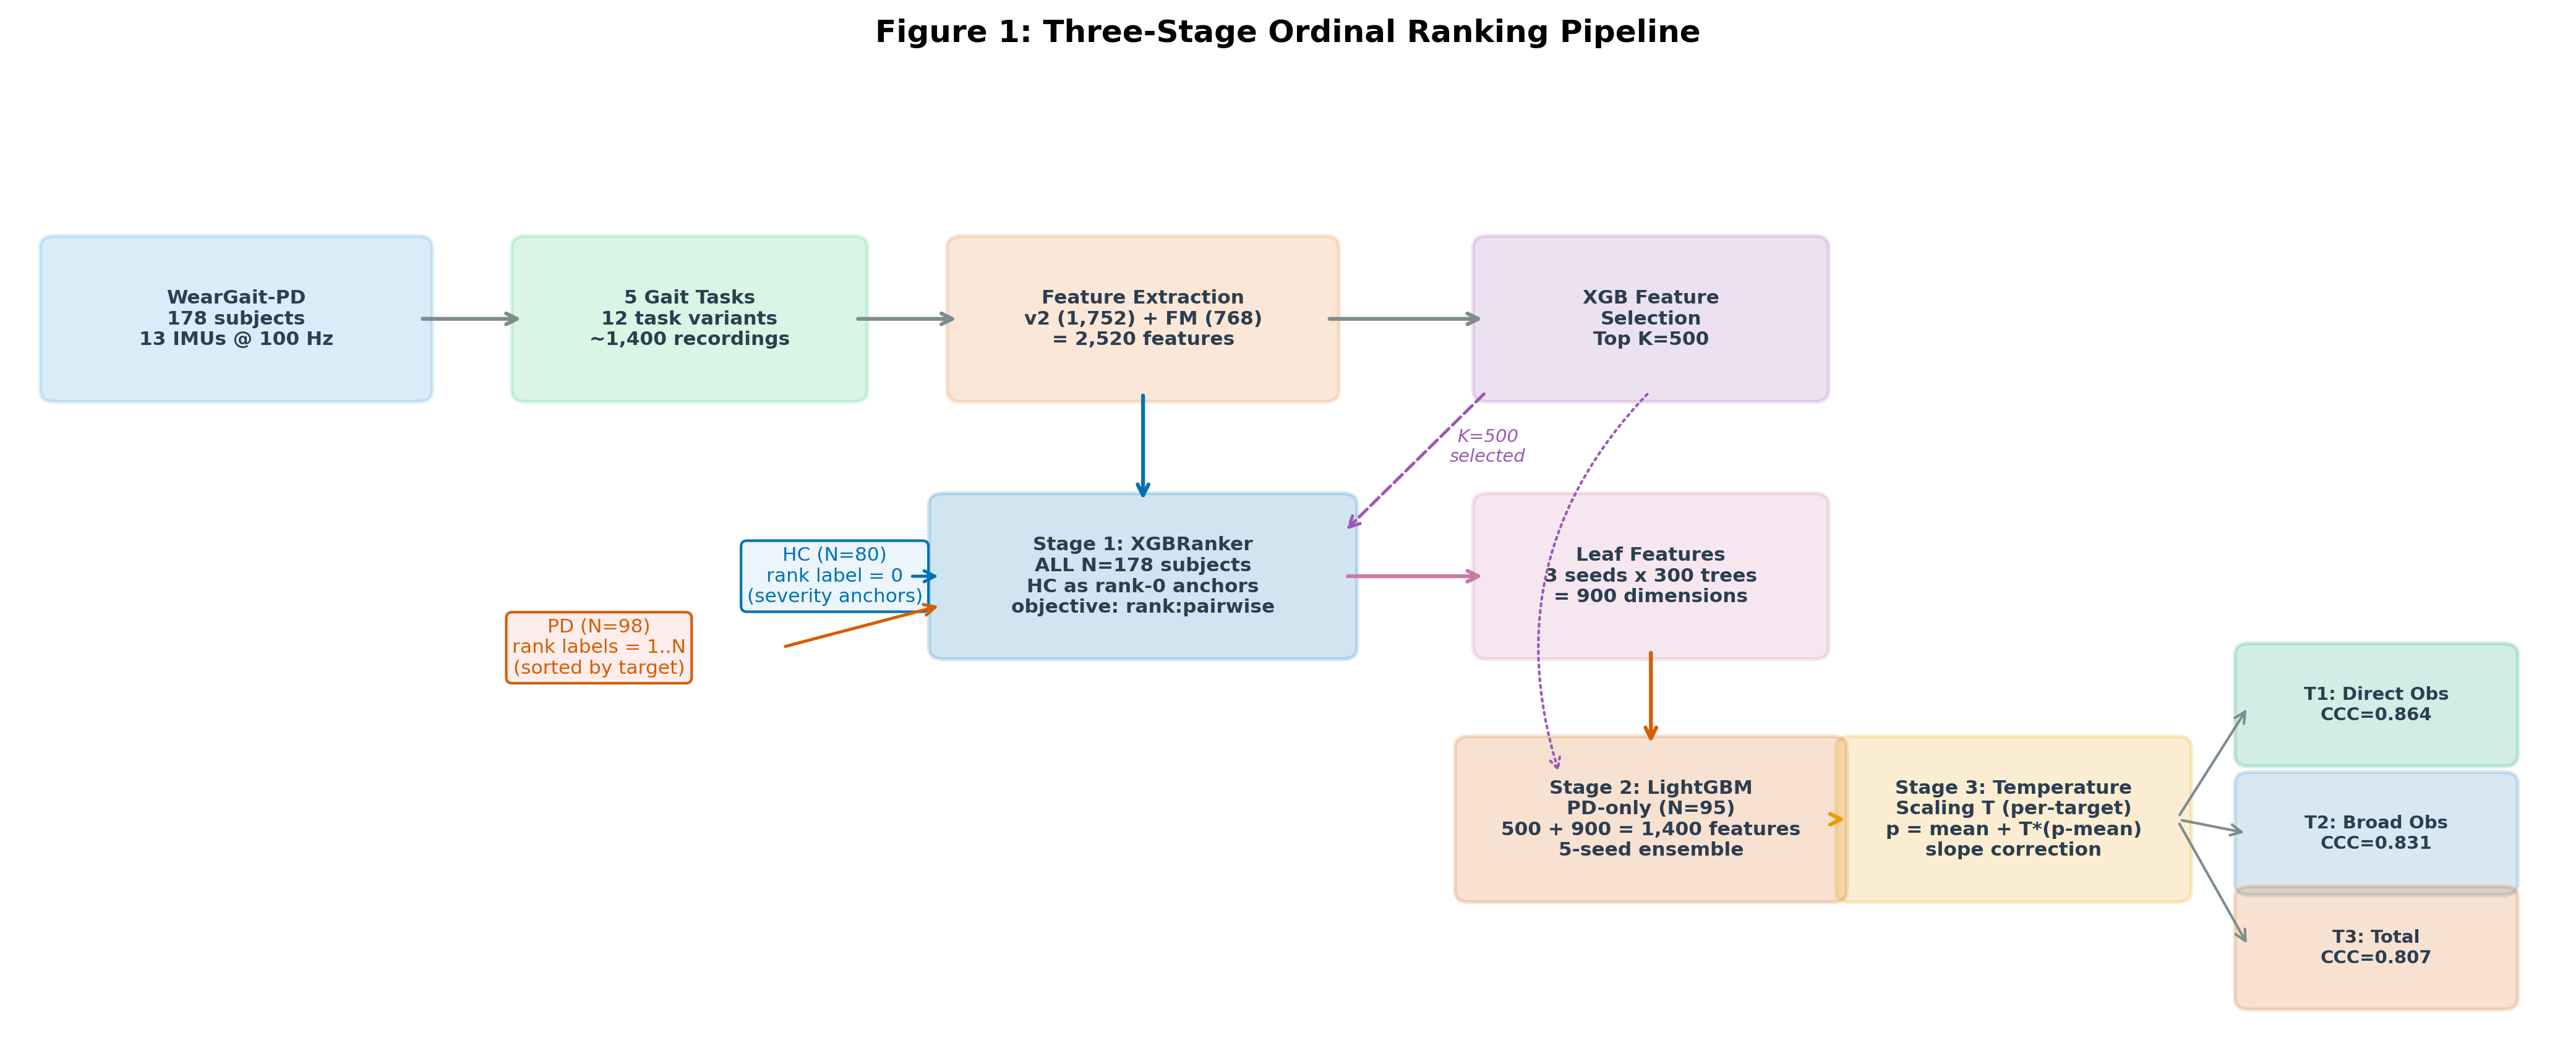
\includegraphics[width=\linewidth]{00_figure_1.png}
\caption{Three-stage prediction pipeline (ordinal ranking + LGB + temperature calibration). Stage~1: XGBRanker trained on all $N=178$ subjects (HC anchored at rank 0, PD subjects ranked by target score) produces leaf features encoding severity ordering. Stage~2: LightGBM regressor trained on PD-only subjects uses original features plus 900 leaf features. Evaluated by PD-only 5-fold stratified CV (primary) and LOOCV (sensitivity).}
\label{fig:pipeline}
\end{figure}

% =========================================================
\section{Results}
% =========================================================

\subsection{Cohort Description}

Of 185 enrolled participants, 178 (98 PD, 80 HC) had complete sensor recordings (Table~\ref{tab:cohort}). PD participants (mean age $66.9\pm8.3$ years, 63M/35F) had moderate motor severity (UPDRS-III $24.4\pm10.9$, range $[0.0, 59.0]$). HC participants were older ($74.6\pm8.5$ years) with lower motor scores ($7.1\pm9.7$). Medication state was not systematically controlled.

\begin{table}[H]
\centering
\caption{Cohort demographics.}
\label{tab:cohort}
\begin{tabular}{lll}
\toprule
\textbf{Characteristic} & \textbf{PD ($N=98$)} & \textbf{HC ($N=80$)} \\
\midrule
Age, years (mean $\pm$ SD)              & $66.9 \pm 8.3$           & $74.6 \pm 8.5$ \\
Sex (M/F)                               & 63M / 35F                & 35M / 45F \\
Height, cm (mean $\pm$ SD)              & $174.2 \pm 10.3$         & $168.1 \pm 17.5$ \\
Weight, kg (mean $\pm$ SD)              & $78.0 \pm 17.2$          & $81.0 \pm 16.8$ \\
UPDRS-III (mean $\pm$ SD)               & $24.4 \pm 10.9$          & $7.1 \pm 9.7$ \\
UPDRS-III range                         & $[0.0, 59.0]$            & $[0.0, 43.0]$ \\
H\&Y (mean $\pm$ SD)                    & $2.15 \pm 0.6$ ($N=95$)  & --- \\
H\&Y distribution                       & 1: 9, 1.5: 1, 2: 58, 2.5: 12, 3: 12, 4: 3 & --- \\
Years since diagnosis (mean $\pm$ SD)   & $7.6 \pm 5.9$ ($[0.0, 26.4]$) & --- \\
DBS                                     & 23                       & --- \\
\bottomrule
\end{tabular}
\end{table}

\subsection{Primary Outcome: Observable Subscore via Ordinal Ranking}

The directly observable subscore (items 3.9--3.14: arising, gait, freezing, postural stability, posture, body bradykinesia; max 24 points) is the primary endpoint. With ordinal ranking plus temperature calibration (P5, PD-only 5-fold CV, $N=95$; Figure~\ref{fig:t1scatter}), the full pipeline achieves $\mathrm{CCC}=0.864$ (95\% BCa CI: $[0.807, 0.906]$), calibration slope $=1.043$, $\mathrm{MAE}=1.156$ ($r=0.877$). This represents a substantial improvement over the P0 baseline ($\mathrm{CCC}=0.70$, slope $=0.508$). While the total-score MCID of 3.25 points (Horvath 2015)\textsuperscript{2} does not directly apply to a 24-point subscore, the MAE of 1.156 represents less than 4\% of the subscore range, suggesting that prospective clinical validation of this subscore endpoint is warranted. A subscore-specific MCID remains to be established.

Ordinal ranking also improves broader targets (Stages~1--2, without temperature scaling): T2 (items 7--14, max 32) achieves $\mathrm{CCC}=0.831$ ($\mathrm{MAE}=1.16$), and T3 (total UPDRS-III) achieves $\mathrm{CCC}=0.807$ ($\mathrm{MAE}=4.46$; Figure~\ref{fig:threetarget}). Comparing all three targets under Stages~1--2 (before temperature scaling), CCC degrades monotonically from $\mathrm{T1}=0.865$ to $\mathrm{T2}=0.831$ to $\mathrm{T3}=0.807$, reflecting increasing inclusion of items unobservable from gait IMU. Temperature scaling (Section~\ref{sec:tempscale}) further improves T1 calibration (slope $0.745 \rightarrow 1.043$) at modest MAE cost. Confirmatory LOOCV analysis ($N=94$) yields consistent results: T1 $\mathrm{CCC}=0.868$, T2 $\mathrm{CCC}=0.852$, T3 $\mathrm{CCC}=0.776$ (Supplementary~S5).

\begin{figure}[H]
\centering
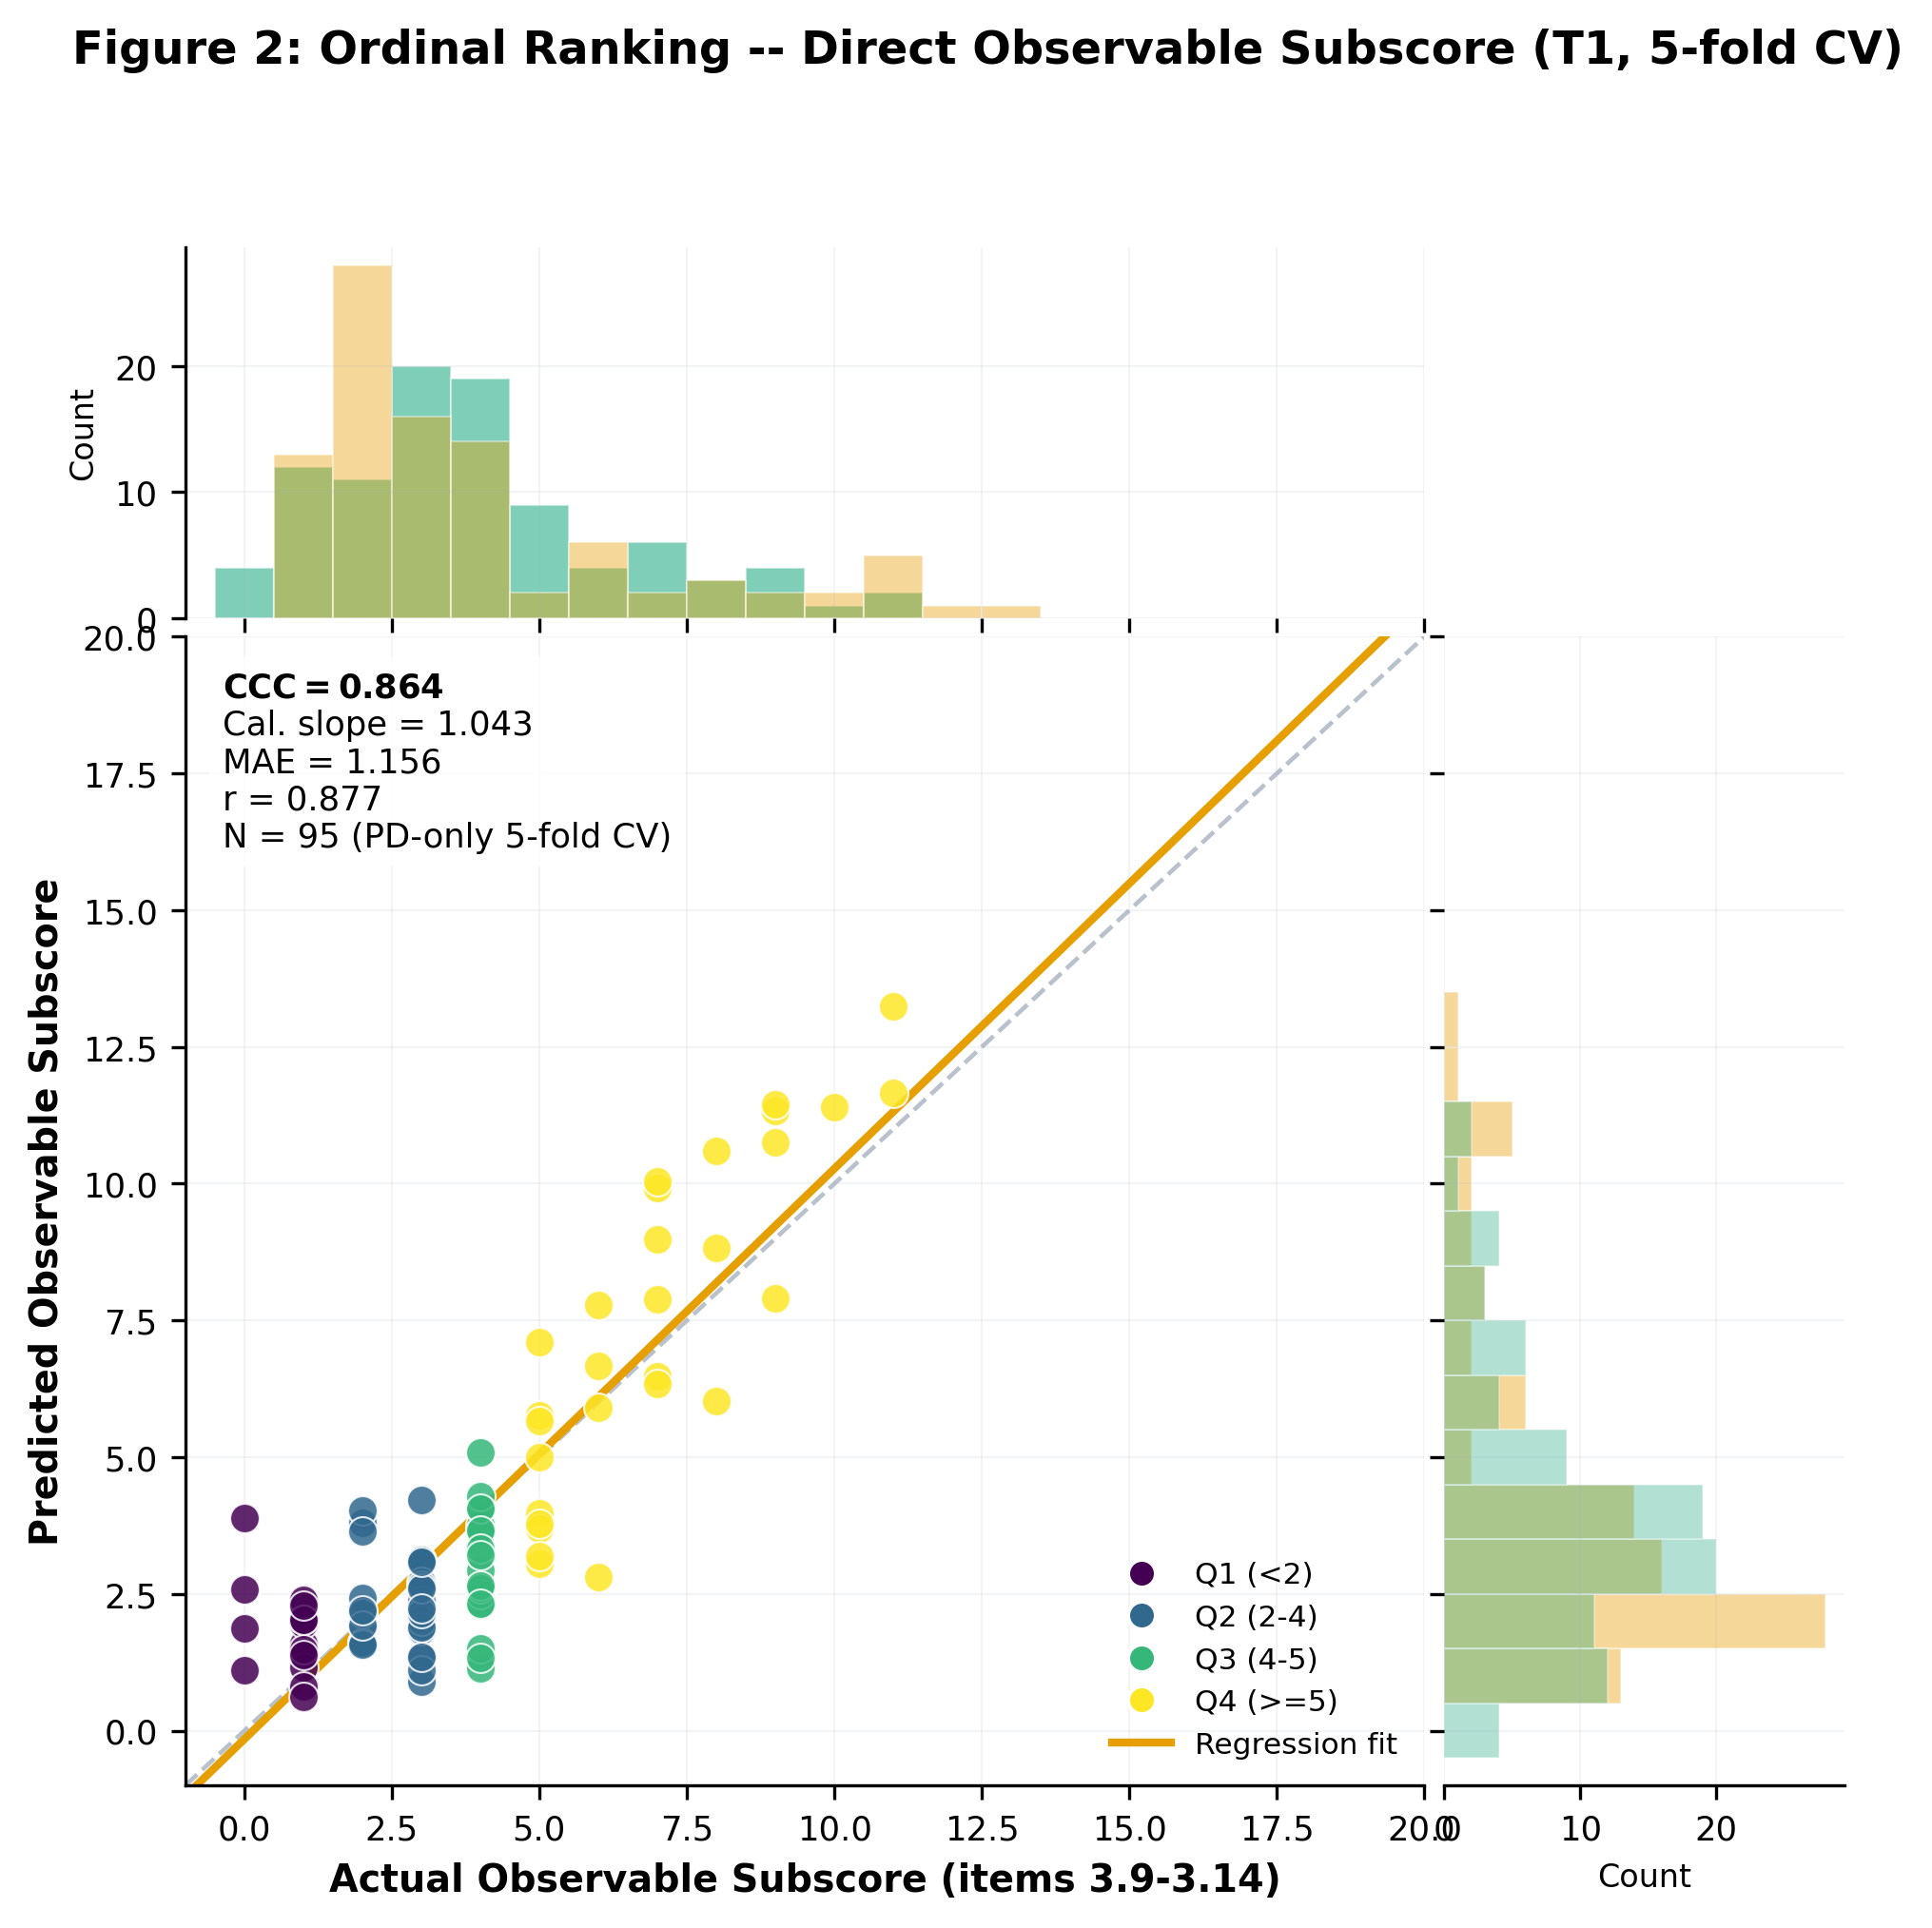
\includegraphics[width=0.85\linewidth]{01_figure_2.png}
\caption{Ordinal ranking predicted versus actual scores for the directly observable subscore (T1, items 3.9--3.14), PD-only 5-fold CV ($N=95$). Points colored by severity quartile. $\mathrm{CCC}=0.864$, calibration slope $=1.043$. Marginal histograms show distribution of actual (green) and predicted (orange) scores.}
\label{fig:t1scatter}
\end{figure}

\begin{figure}[H]
\centering
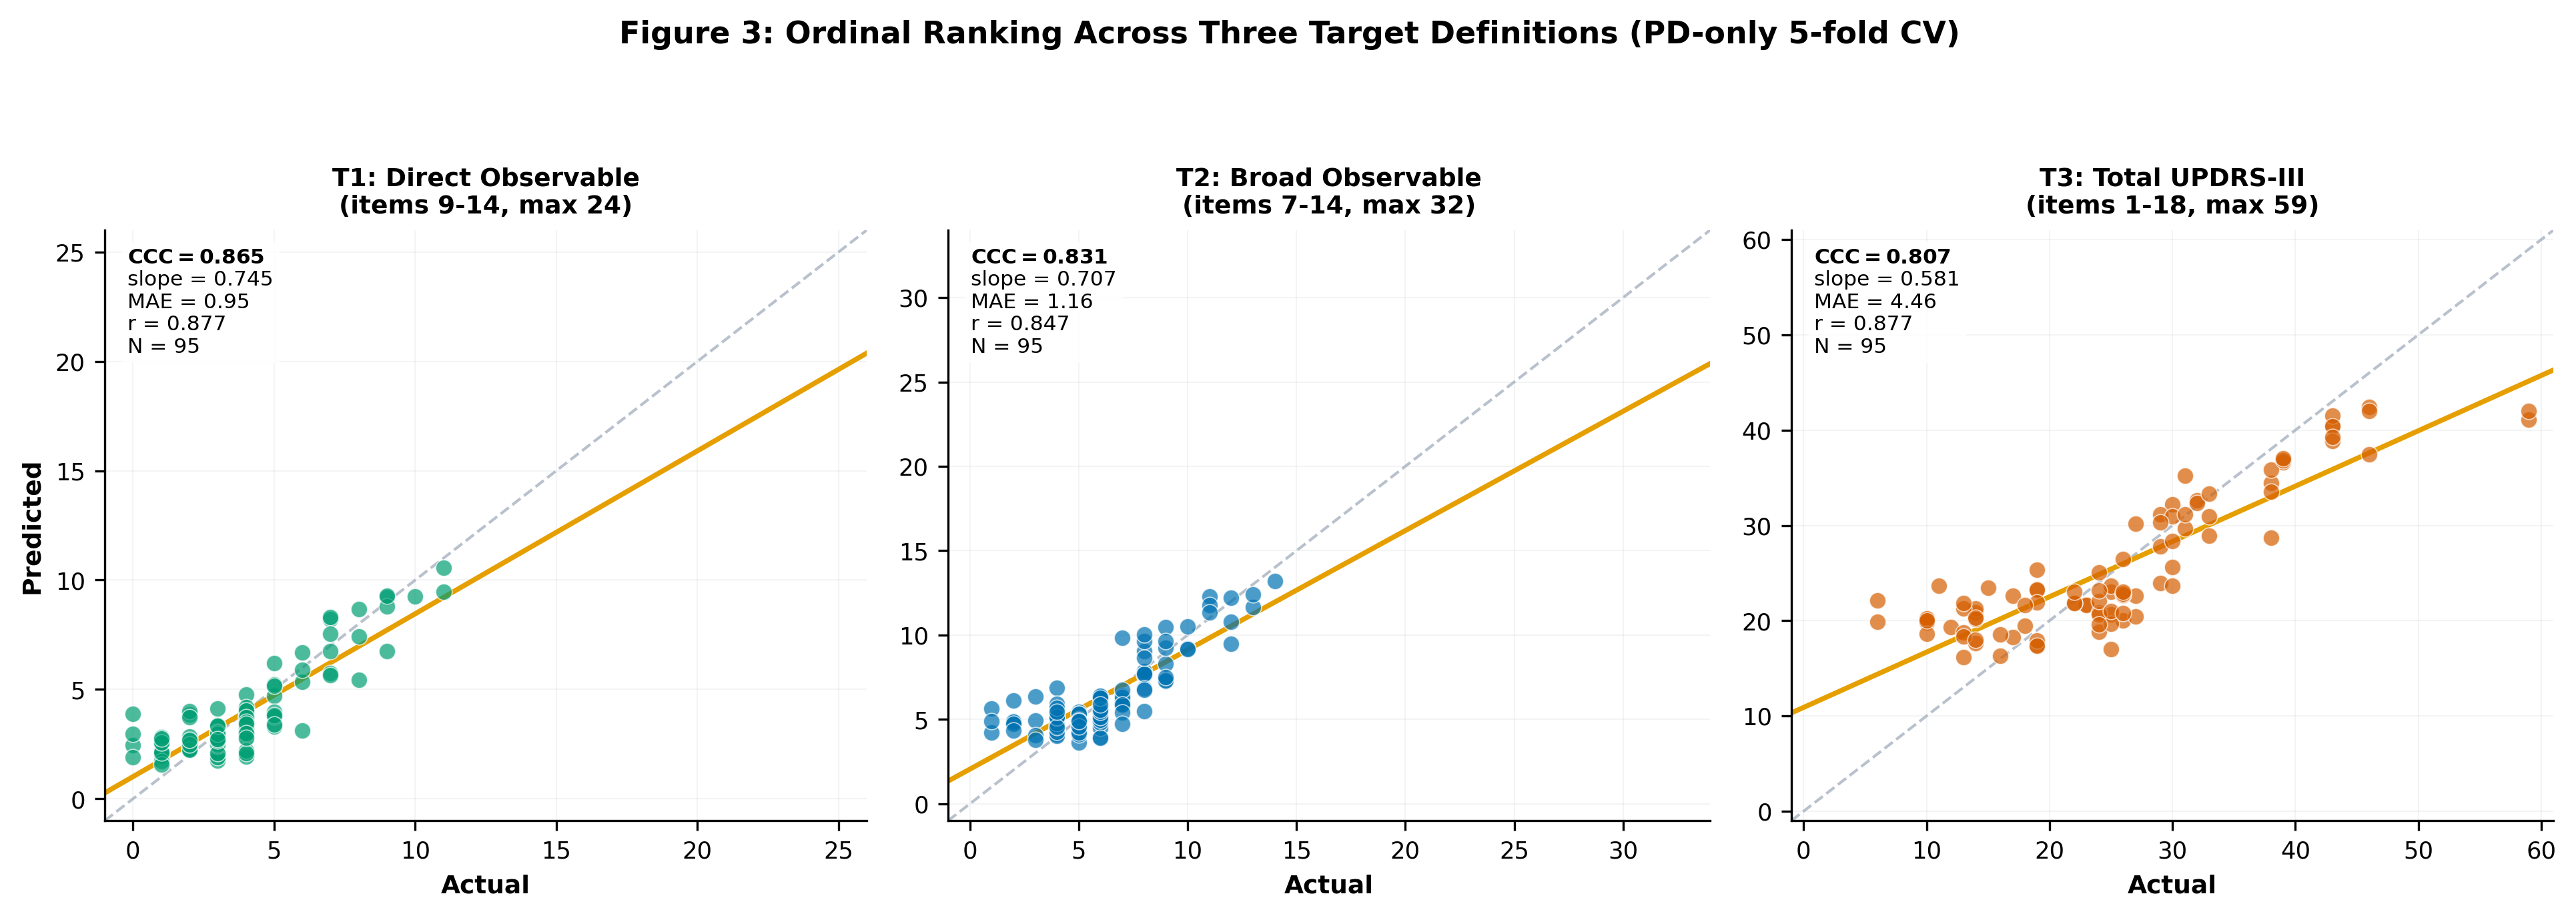
\includegraphics[width=\linewidth]{02_figure_3.png}
\caption{Ordinal ranking (Stages~1--2, without temperature scaling) across three target definitions (PD-only 5-fold CV, $N=95$). Left: T1 direct observable ($\mathrm{CCC}=0.865$). Center: T2 broad observable ($\mathrm{CCC}=0.831$). Right: T3 total UPDRS-III ($\mathrm{CCC}=0.807$). All panels show Stages~1--2 predictions for consistent cross-target comparison. CCC degrades monotonically as targets include more items unobservable from gait sensors. Per-target temperature scaling results in Supplementary Figure~S5.}
\label{fig:threetarget}
\end{figure}

\subsection{Observability Structure}

We decomposed the 18 MDS-UPDRS-III items into three tiers based on whether the assessed motor sign is physically manifest during gait. This exploratory analysis uses the same 5-fold CV protocol as the primary outcome (Table~\ref{tab:obs}, Figure~\ref{fig:obs}). The directly observable subscore achieves $\mathrm{CCC}=0.864$ (Section~2.2). For partial and not-observable tiers, prediction on a restricted subset ($N=90$, requiring complete scores for all 18 items) yields: partially observable $\mathrm{CCC}=0.730$ ($\mathrm{MAE}=2.59$), not observable $\mathrm{CCC}=0.759$ ($\mathrm{MAE}=2.10$).

The structure is two-level rather than monotonically three-level: directly observable items ($\mathrm{CCC}=0.864$) substantially exceed both partially observable ($\mathrm{CCC}=0.730$) and not-observable ($\mathrm{CCC}=0.759$) tiers, but the ordering between the latter two is not significant (Williams test for ordered alternatives: $p=0.69$). The not-observable tier slightly exceeds the partially observable tier, which may reflect that not-observable items (speech, facial expression, rigidity) correlate with overall disease severity through shared pathophysiology, while partially observable items (hand movements, pronation-supination, toe tapping) are limb-specific motor signs with higher inter-subject variability. We therefore characterize the observability structure as direct $\gg$ rest, rather than claiming a monotonic gradient. Ordinal ranking improves all three tiers substantially over baseline: direct CCC $0.545 \rightarrow 0.864$; partial CCC $0.055 \rightarrow 0.730$; unobs CCC $0.176 \rightarrow 0.759$.

Per-item analysis (Figure~\ref{fig:items}) confirms this structure: the highest-correlation items are predominantly directly observable gait items. Feature importance for the observable subscore (Figure~\ref{fig:featimp}) shows clinically coherent sensor-item alignment: foot sensors (R\_DorsalFoot), lower back, and trunk (Xiphoid) drive predictions, while foundation model embedding dimensions provide complementary temporal patterns.

\begin{figure}[H]
\centering
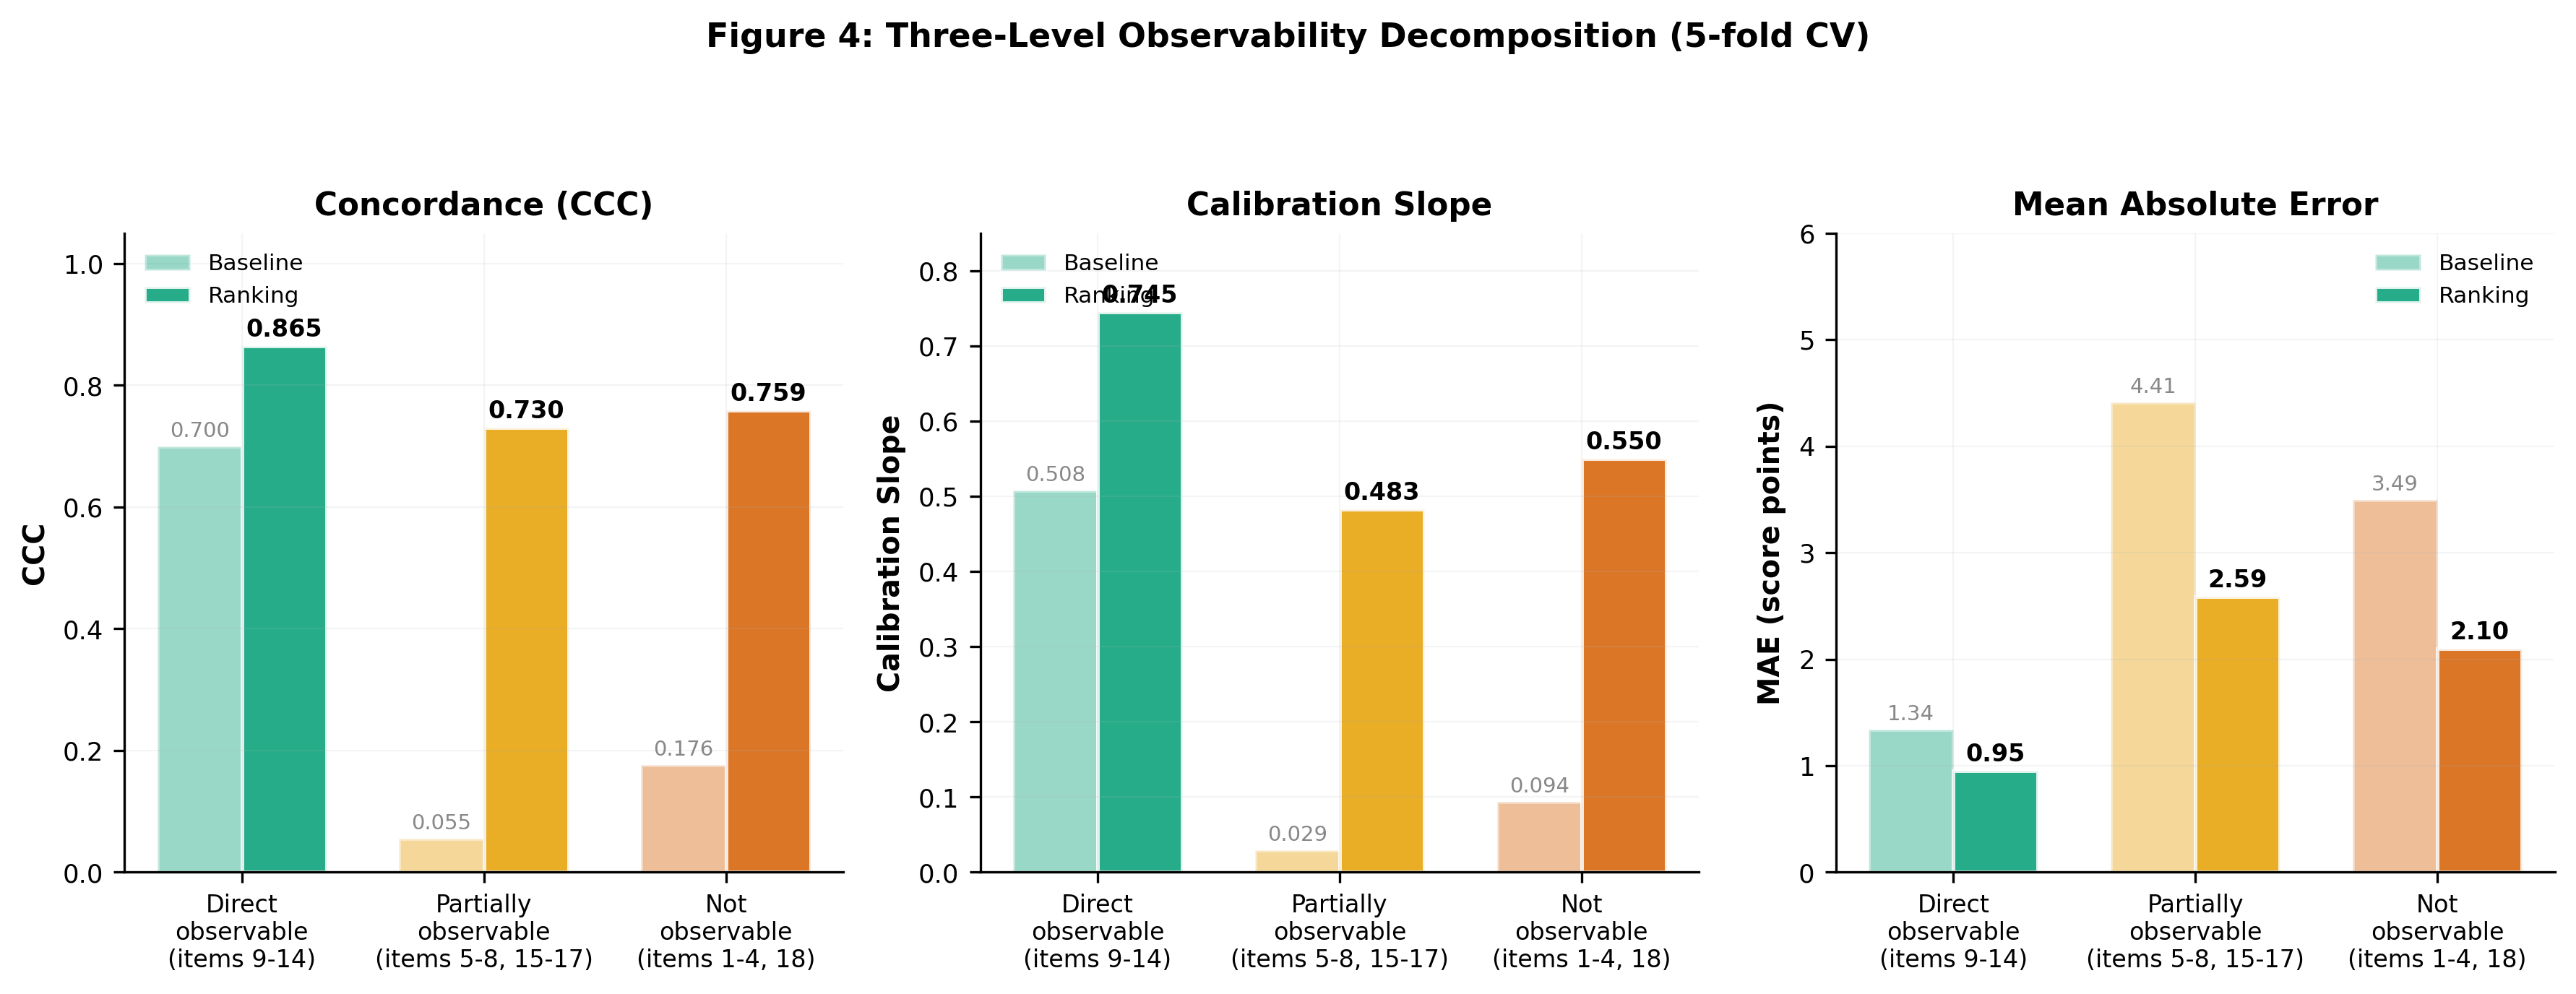
\includegraphics[width=\linewidth]{03_figure_4.png}
\caption{Three-tier observability decomposition (5-fold CV). CCC, calibration slope, and MAE show a two-level structure: directly observable items are well-predicted under both baseline and ranking conditions, while partially observable and not-observable tiers show uniformly lower CCC (ordering between them is not significant, $p=0.69$). This is a modality constraint: rigidity (item 3.3), speech (3.1), and facial expression (3.2) cannot be measured by body-worn inertial sensors during gait.}
\label{fig:obs}
\end{figure}

\begin{table}[H]
\centering
\caption{Three-level observability decomposition (PD-only 5-fold CV).}
\label{tab:obs}
\small
\resizebox{\textwidth}{!}{%
\begin{tabular}{llrrrrrr}
\toprule
\textbf{Tier} & \textbf{Items} & \textbf{Base.\ CCC} & \textbf{Base.\ MAE} & \textbf{Rank.\ CCC} & \textbf{Rank.\ MAE} & \textbf{Rank.\ slope} & \textbf{Rank.\ $r$} \\
\midrule
Directly observable    & 3.9--3.14            & 0.700 & 1.336 & \textbf{0.864} & 1.156 & 1.043 & 0.877 \\
Partially observable   & 3.5--3.8, 3.15--3.17 & 0.055 & 4.411 & \textbf{0.730} & 2.590 & 0.483 & 0.849 \\
Not observable         & 3.1--3.4, 3.18       & 0.176 & 3.494 & \textbf{0.759} & 2.097 & 0.550 & 0.823 \\
\bottomrule
\end{tabular}
}%
\tabnote{Directly observable row uses the primary pipeline ($N=95$, identical to Section~2.2). Partial and not-observable rows use a restricted subset ($N=90$) requiring complete scores for all 18 items. All evaluated under 5-fold CV.}
\end{table}

\begin{figure}[H]
\centering
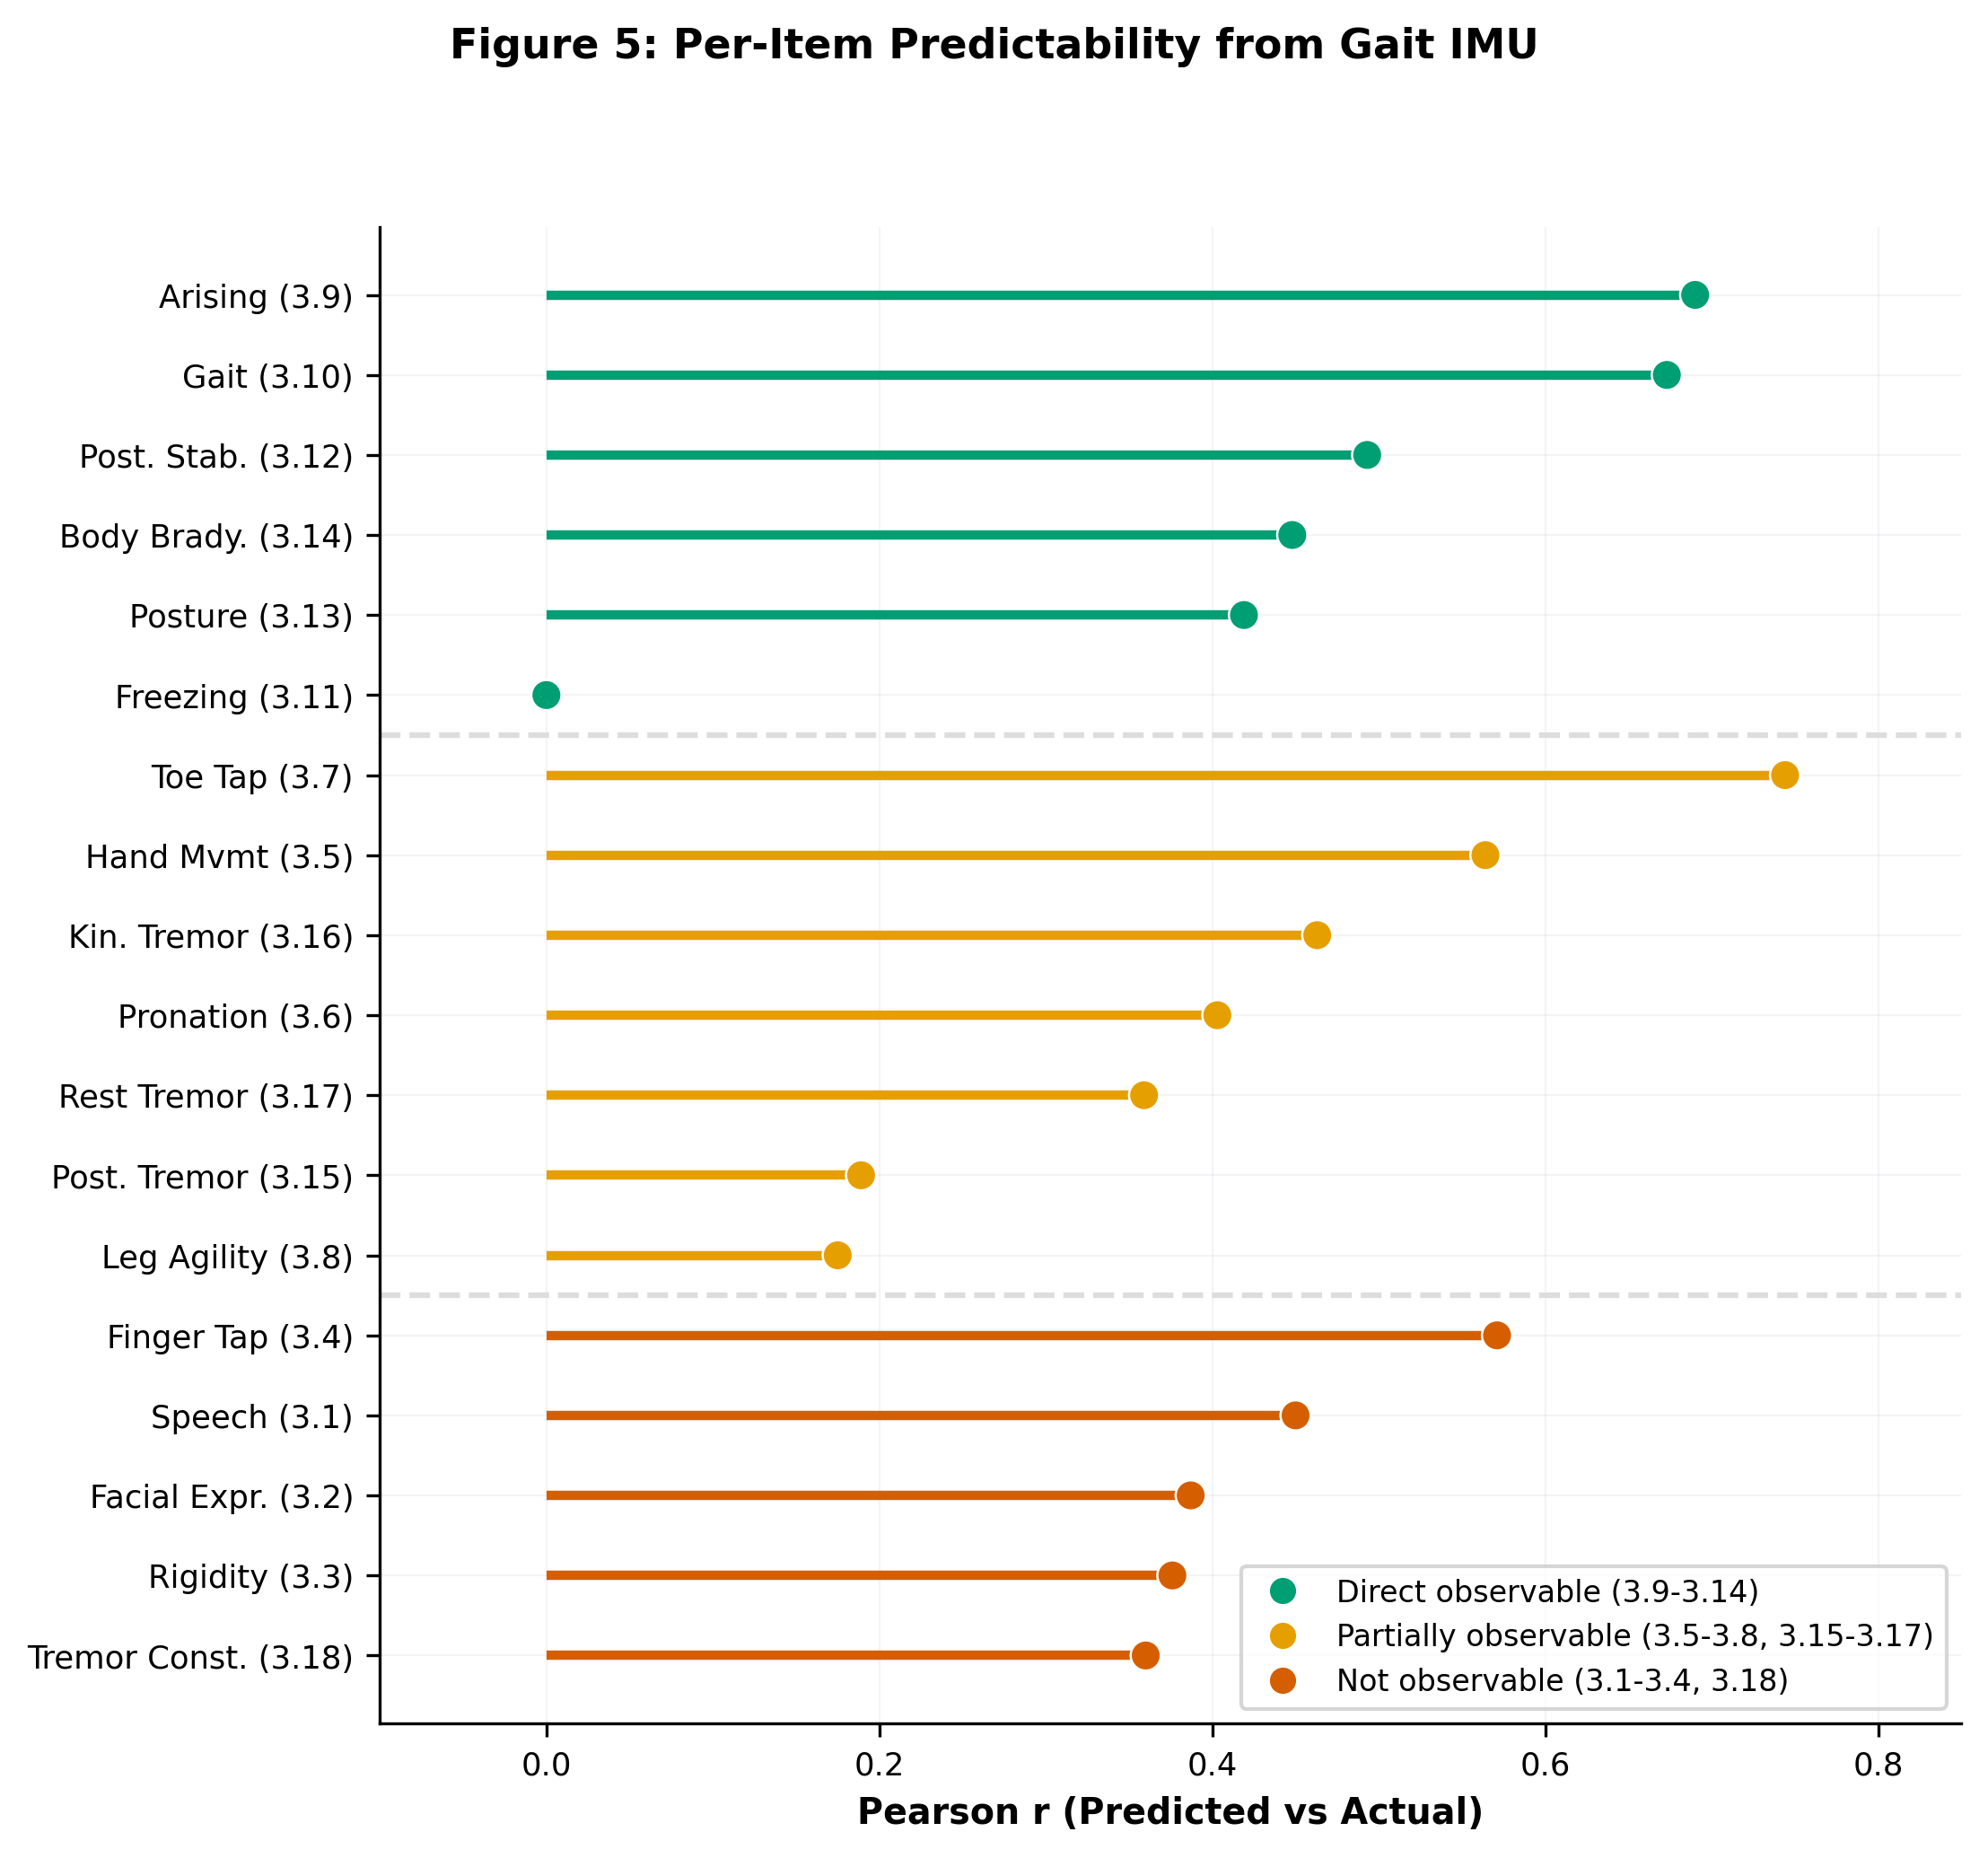
\includegraphics[width=\linewidth]{04_figure_5.png}
\caption{Per-item predictability ranked by Pearson $r$, colored by observability tier. Green: directly observable from gait; orange: partially observable; red: not observable. Dashed lines separate tiers. The two-level structure is apparent: direct items cluster at higher $r$ values, while partial and unobservable items intermix.}
\label{fig:items}
\end{figure}

\begin{figure}[H]
\centering
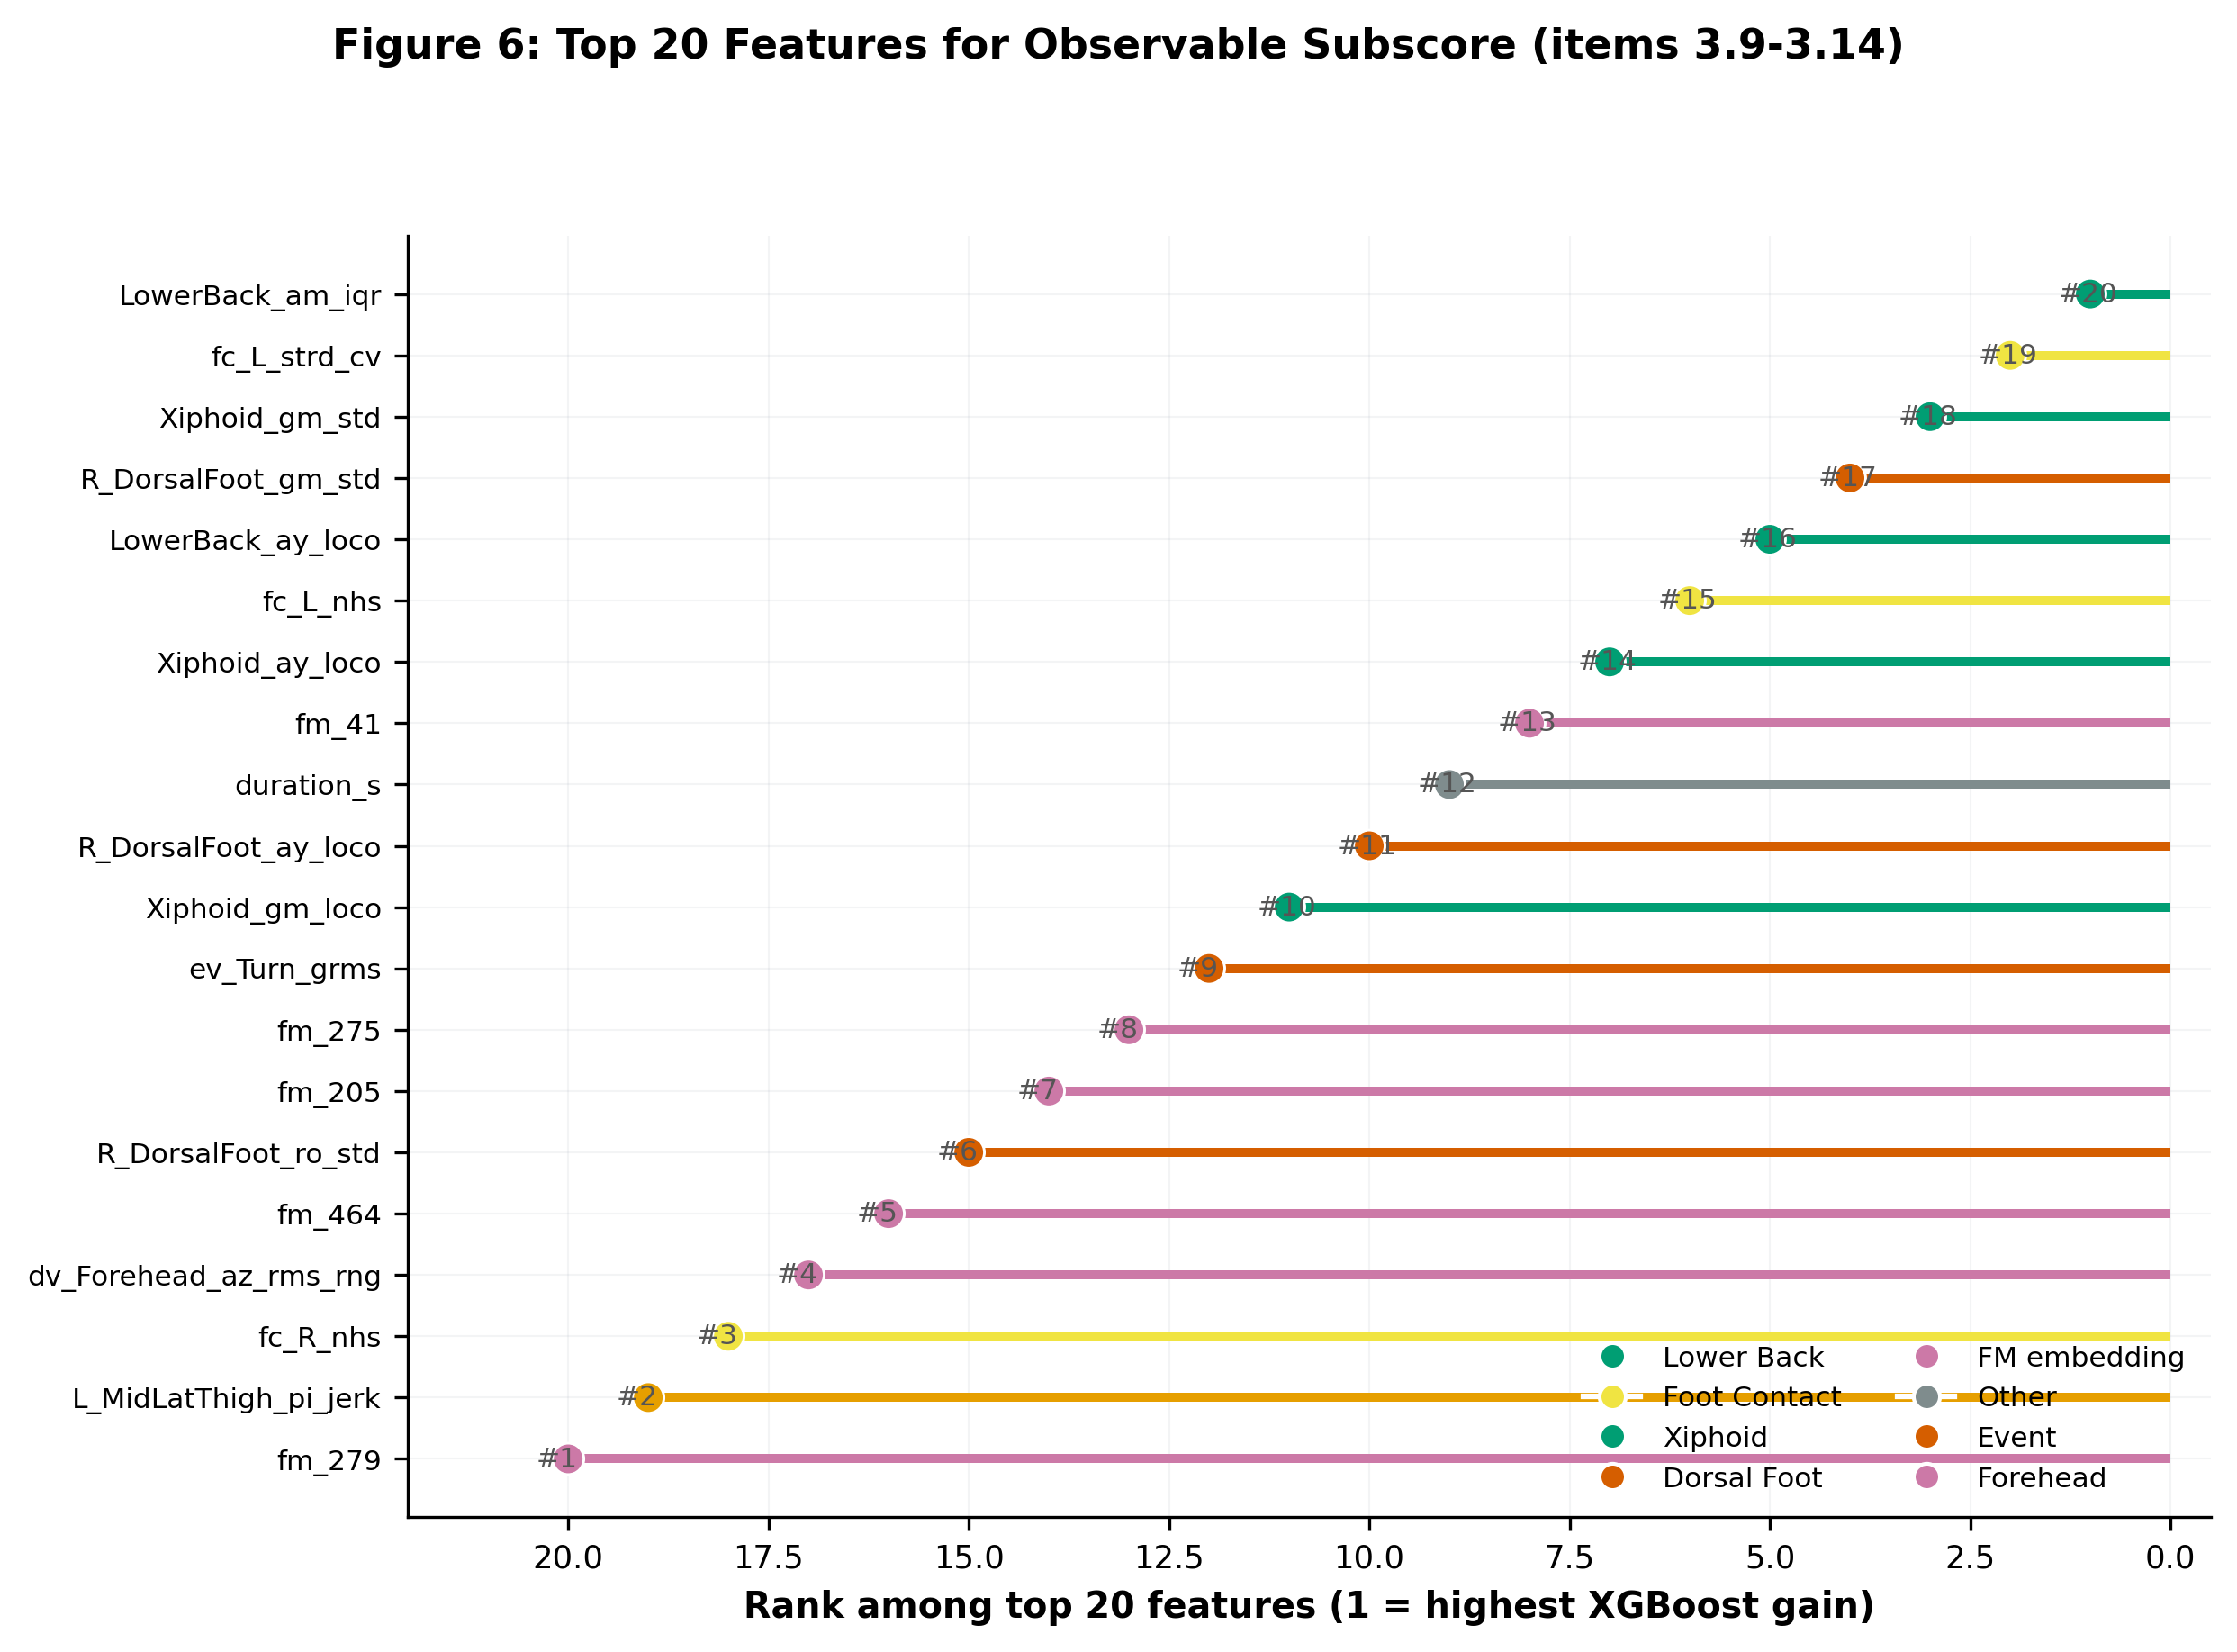
\includegraphics[width=\linewidth]{05_figure_6.png}
\caption{Top 20 features by XGBoost gain importance for the observable subscore model, colored by anatomical source. Foot and trunk sensors dominate, with FM embedding dimensions (\texttt{fm\_*}) providing complementary temporal features.}
\label{fig:featimp}
\end{figure}

\subsection{Calibration Fix: Temperature Scaling}
\label{sec:tempscale}

Although ordinal ranking substantially improves CCC, the calibration slope remains below 1.0 (slope $=0.745$ for T1 5-fold CV), indicating residual prediction compression. The root cause is mechanical: LightGBM leaf averaging with \texttt{min\_data\_in\_leaf}$=8$ on $N\approx 80$ training subjects compresses extreme predictions toward the mean, and multi-seed ensemble averaging adds further compression.

Post-hoc temperature scaling with a single parameter $T=1.4$ corrects this compression. The scaled prediction is: $p_{\mathrm{scaled}} = \mu_{\mathrm{train}} + T \times (p_{\mathrm{ensemble}} - \mu_{\mathrm{train}})$, where $\mu_{\mathrm{train}}$ is the population mean of the training set. This stretches predictions outward from the mean, counteracting the ensemble compression. $T$ is selected as the value from a grid $[1.0, 1.1, \ldots, 2.0]$ that minimizes $|\text{cal\_slope} - 1.0|$ on T1 LOOCV predictions. Because $T$ was tuned on T1, temperature scaling is applied only to T1 results; T2 and T3 report Stages~1--2 (ranking + regression) without temperature scaling throughout this paper.

Temperature scaling improves calibration slope from 0.745 to 0.967 and CCC from 0.868 to 0.882 (LOOCV, T1; Table~S8). MAE increases slightly ($0.986 \rightarrow 1.162$), reflecting the trade-off between calibration and point accuracy inherent in stretching predictions: extreme-quintile patients are better calibrated at the cost of modest accuracy loss in the mid-range. Among seven calibration methods tested (CCC custom loss, quantile regression, KNN, variance penalty, conformal quantile, Ridge, temperature), temperature scaling achieved the best combination of CCC (0.882) and calibration slope (0.967) with a single interpretable parameter (Table~S8).

\subsection{Total UPDRS-III as Context}

Total UPDRS-III prediction illustrates the structural ceiling that motivates the observable subdomain focus. With ordinal ranking (Stages~1--2, 5-fold CV), T3 achieves $\mathrm{CCC}=0.807$ ($\mathrm{MAE}=4.46$), substantially above the P0 baseline ($\mathrm{CCC}=0.186$, $\mathrm{MAE}=8.09$). In PD-only 10-split CV ($N=98$, Table~\ref{tab:total}), a demographic Ridge baseline (age, sex, disease duration) achieved $\mathrm{MAE}=7.44\pm0.75$, matching all pre-ranking IMU models. Partial correlation $r=0.36$ ($p_{\mathrm{adj}}=0.002$) confirms genuine IMU signal beyond demographics, but this signal is diluted by 12 partially or non-observable items constituting 82\% of the total score range. After ordinal ranking, IMU clearly surpasses demographics: T3 $\mathrm{MAE}=4.46$ vs demographic LOOCV $\mathrm{MAE}=7.86$.

\begin{table}[H]
\centering
\caption{Total UPDRS-III prediction results (PD-only evaluation).}
\label{tab:total}
\small
\resizebox{\textwidth}{!}{%
\begin{tabular}{lllrrrr}
\toprule
\textbf{Model} & \textbf{Evaluation} & \textbf{$N$} & \textbf{MAE} & \textbf{CCC} & \textbf{$r$} & \textbf{Cal.\ slope} \\
\midrule
\multicolumn{7}{l}{\emph{PD-only 10-split cross-validation}} \\
Demographic Ridge     & 10-split & 98 & $7.44 \pm 0.75$ &  0.326 & --- & --- \\
v2 Handcrafted LGB    & 10-split & 98 & $8.42 \pm 0.69$ & $-0.004$ & --- & --- \\
v2+FM Stack           & 10-split & 98 & $8.57 \pm 0.96$ & $-0.019$ & --- & --- \\
\addlinespace
\multicolumn{7}{l}{\emph{PD-only leave-one-out cross-validation}} \\
FM Stack (baseline)   & LOOCV    & 98 & 8.15            & 0.369 & 0.429 & 0.256 \\
Demographic Ridge     & LOOCV    & 98 & 7.86            & 0.338 & 0.427 & 0.211 \\
\addlinespace
\multicolumn{7}{l}{\emph{Anti-compression methods (PD-only, 5-split, Stages~1--2)}} \\
P0 Baseline           & 5-split  & 95 & 8.09            & 0.186 & 0.297 & 0.104 \\
\textbf{P5 Ordinal Ranking} & \textbf{5-split} & \textbf{95} & \textbf{4.46} & \textbf{0.807} & \textbf{0.877} & \textbf{0.581} \\
\bottomrule
\end{tabular}
}%
\tabnote{P0 baseline and P5 ordinal ranking use the same 5-split evaluation protocol for direct comparison. P5 row shows Stages~1--2 (ordinal ranking + regression, without temperature scaling; temperature $T=1.4$ was tuned on T1 only). P5 uses healthy controls for ranking representation learning only; final evaluation is PD-only. Confirmatory LOOCV ($N=94$): $\mathrm{CCC}=0.776$, $\mathrm{MAE}=4.65$ (Table~S7).}
\end{table}

\begin{table}[H]
\centering
\caption{Severity-stratified prediction (baseline, PD-only FM LOOCV, $N=98$).}
\label{tab:severity}
\resizebox{\textwidth}{!}{%
\begin{tabular}{lrrrrrr}
\toprule
\textbf{Quartile} & \textbf{$N$} & \textbf{MAE} & \textbf{CCC} & \textbf{Bias} & \textbf{Mean True} & \textbf{Mean Pred} \\
\midrule
Q1 ($<$12)   &  9 & 14.09 & 0.141 & $+14.1$ &  6.2 & 20.3 \\
Q2 (12--20)  & 26 &  5.96 & 0.068 &  $+4.5$ & 15.6 & 20.1 \\
Q3 (20--35)  & 46 &  5.94 & 0.152 &  $-4.0$ & 26.8 & 22.7 \\
Q4 ($>$35)   & 17 & 14.30 & 0.138 & $-14.3$ & 41.2 & 26.9 \\
\bottomrule
\end{tabular}
}%
\tabnote{Bias $=$ mean(predicted $-$ actual). Severe regression to the mean: Q1 overpredicted by $+14$, Q4 underpredicted by $-14$. Pre-ranking baseline.}
\end{table}

\subsection{Age Confound and HC Ablation Sensitivity}

Because HC participants were older than PD participants (74.6 vs 66.9 years), we conducted two sensitivity analyses to rule out age-driven confounding and to assess the specific contribution of HC subjects to ordinal ranking.

\textbf{Age confound analysis (Table~\ref{tab:age}).} We compared ordinal ranking using the full HC cohort ($N=80$, mean age 74.6y) against an age-matched HC subset ($N=46$, mean age 68.9y, $p=0.0905$ vs PD). Age-matched HC gives T1 $\mathrm{CCC}=0.868$ vs full HC $\mathrm{CCC}=0.858$---age is not driving the ranking improvement. Partial correlation controlling for age yields $r=0.849$ ($p<0.001$), confirming that ordinal ranking predictions reflect motor severity, not age. Age-stratified within-PD analysis shows consistent performance across all PD age strata (Table~\ref{tab:agestrat}): young $\mathrm{CCC}=0.730$, middle $\mathrm{CCC}=0.706$, older $\mathrm{CCC}=0.911$.

\textbf{HC ablation (Table~\ref{tab:hc}).} We compared three conditions: P0 baseline (no ranking), P5 with PD-only ranking (no HC), and P5 with PD+HC ranking. PD-only ranking achieves T1 $\mathrm{CCC}=0.857$, nearly identical to PD+HC ranking $\mathrm{CCC}=0.858$. Both substantially exceed the P0 baseline ($\mathrm{CCC}=0.673$). This demonstrates that the ordinal ranking-to-leaf-feature transformation itself is the primary driver of the improvement; HC subjects provide incremental calibration anchoring but are not required for the core benefit.

\begin{table}[H]
\centering
\caption{Age confound sensitivity analysis for ordinal ranking (5-fold CV, T1 observable subscore).}
\label{tab:age}
\small
\resizebox{\textwidth}{!}{%
\begin{tabular}{lrrrrrrrrr}
\toprule
\textbf{HC Config} & $N_{\mathrm{HC}}$ & \textbf{HC Age} & \textbf{Age $p$} & \textbf{T1 CCC} & \textbf{T1 MAE} & \textbf{T1 $r$} & \textbf{T1 slope} & \textbf{T3 CCC} & \textbf{T3 MAE} \\
\midrule
Full HC         & 80 & 74.6 & $<0.001$ & \textbf{0.858} & 0.986 & 0.874 & 0.718 & 0.763 & 4.968 \\
Age-matched HC  & 46 & 68.9 & 0.0905   & \textbf{0.868} & 0.978 & 0.880 & 0.744 & 0.751 & 4.998 \\
\bottomrule
\end{tabular}
}%
\tabnote{Age-matched subset retains HC with age $\le$ PD 75th percentile $+$ 5 years (threshold 78y). Partial correlation of ordinal ranking predictions controlling for age: $r=0.849$ ($p<0.001$). Controlling for age $+$ disease duration: $r=0.823$ ($p<0.001$).}
\end{table}

\begin{table}[H]
\centering
\caption{Age-stratified within-PD evaluation (ordinal ranking T1, 5-fold CV).}
\label{tab:agestrat}
\begin{tabular}{lrrrr}
\toprule
\textbf{Age Stratum} & \textbf{$N$} & \textbf{CCC} & \textbf{MAE} & \textbf{$r$} \\
\midrule
young ($<65$y)     & 31 & 0.730 & 0.925 & 0.781 \\
middle (65--71y)   & 29 & 0.706 & 1.094 & 0.727 \\
older ($\ge 71$y)  & 35 & 0.911 & 0.951 & 0.927 \\
\bottomrule
\end{tabular}
\tabnote{Ordinal ranking produces accurate predictions across all PD age strata, confirming that performance is not driven by age-related gait rather than disease severity.}
\end{table}

\begin{table}[H]
\centering
\caption{HC ablation: contribution of healthy controls to ordinal ranking (5-fold CV).}
\label{tab:hc}
\small
\resizebox{\textwidth}{!}{%
\begin{tabular}{lrrrrrrrr}
\toprule
\textbf{Method} & $N_{\mathrm{HC}}$ & \textbf{T1 CCC} & \textbf{T1 MAE} & \textbf{T1 slope} & \textbf{T1 $r$} & \textbf{T3 CCC} & \textbf{T3 MAE} & \textbf{T3 slope} \\
\midrule
P0: Baseline (no ranking) &  0 & 0.673 & 1.380 & 0.477 & 0.741 & 0.209 & 8.032 & 0.116 \\
P5: PD-only ranking       &  0 & 0.857 & 1.013 & 0.746 & 0.867 & 0.789 & 4.591 & 0.572 \\
P5: PD+HC ranking         & 80 & 0.858 & 0.986 & 0.718 & 0.874 & 0.763 & 4.968 & 0.544 \\
\bottomrule
\end{tabular}
}%
\tabnote{PD-only ranking (no HC) produces nearly identical T1 performance to PD+HC ranking, demonstrating that the ranking mechanism itself drives the improvement. HC subjects contribute calibration anchoring but are not required for the core benefit. P0 baseline in this table uses a different random split from the primary P0 baseline (Table~S2); minor metric variation is expected.}
\end{table}

\subsection{Sensor Reduction: Clinical Deployment Roadmap}

To bridge the gap between research (13 body-worn IMUs) and clinical deployment, we systematically evaluated 22 sensor configurations spanning 1 to 13 sensors (Table~\ref{tab:sensor22}, Figure~\ref{fig:pareto}). Initial 5-fold screening revealed an apparent ``fewer sensors equal better'' paradox: several reduced configurations outperformed the 13-sensor reference on CCC. To resolve this, we conducted $10\times 5$-fold repeated cross-validation on four key configurations (Table~\ref{tab:sensorrepeated}, Figure~\ref{fig:forest}), with Nadeau--Bengio corrected non-inferiority testing ($\delta=0.05$ CCC).

The 5-sensor minimal set (lower back, bilateral wrists, bilateral ankles) is the only configuration non-inferior to all\_13 across all three targets (T1: $\Delta\mathrm{CCC}=-0.018$, $p_{\mathrm{NI}}=0.003$; T2: $\Delta\mathrm{CCC}=+0.013$, $p_{\mathrm{NI}}<0.001$; T3: $\Delta\mathrm{CCC}=+0.017$, $p_{\mathrm{NI}}=0.001$). Wrists+ankles (4 sensors) is statistically superior for T3 ($\Delta\mathrm{CCC}=+0.030$, $p_{\mathrm{sup}}=0.006$) and superior for T2 ($p_{\mathrm{sup}}=0.010$), but non-inferior (not superior) for T1. A single lower back sensor achieves non-inferiority for T1 and T2 but fails for T3 ($\Delta\mathrm{CCC}=-0.039$, $p_{\mathrm{NI}}=0.268$), indicating that extremity sensors are required for total UPDRS-III prediction.

The initial ``fewer$=$better'' paradox was a winner's curse artifact: in single-round 5-fold screening, \texttt{lower\_back\_1} showed $\mathrm{CCC}=0.884$ vs all\_13 $\mathrm{CCC}=0.862$ for T1. With $10\times 5$-fold repeated CV, this gap shrank to $+0.013$ ($p_{\mathrm{superiority}}=0.16$, not significant), confirming that the original screening inflated the apparent advantage.

FM decomposition (Table~\ref{tab:fmdecomp}, Figure~\ref{fig:fmdecomp}) reveals that FM embeddings are largely redundant when combined with handcrafted features: FM-only prediction yields $\mathrm{CCC}\approx -0.01$ (random). FM provides meaningful benefit only for \texttt{wrists\_ankles\_4} on T3 ($\Delta\mathrm{CCC}=+0.058$), where the reduced sensor count limits handcrafted feature diversity and FM compensates. The ``fewer$=$better'' pattern is thus driven by handcrafted feature quality versus quantity, not by FM representation.

\begin{figure}[H]
\centering
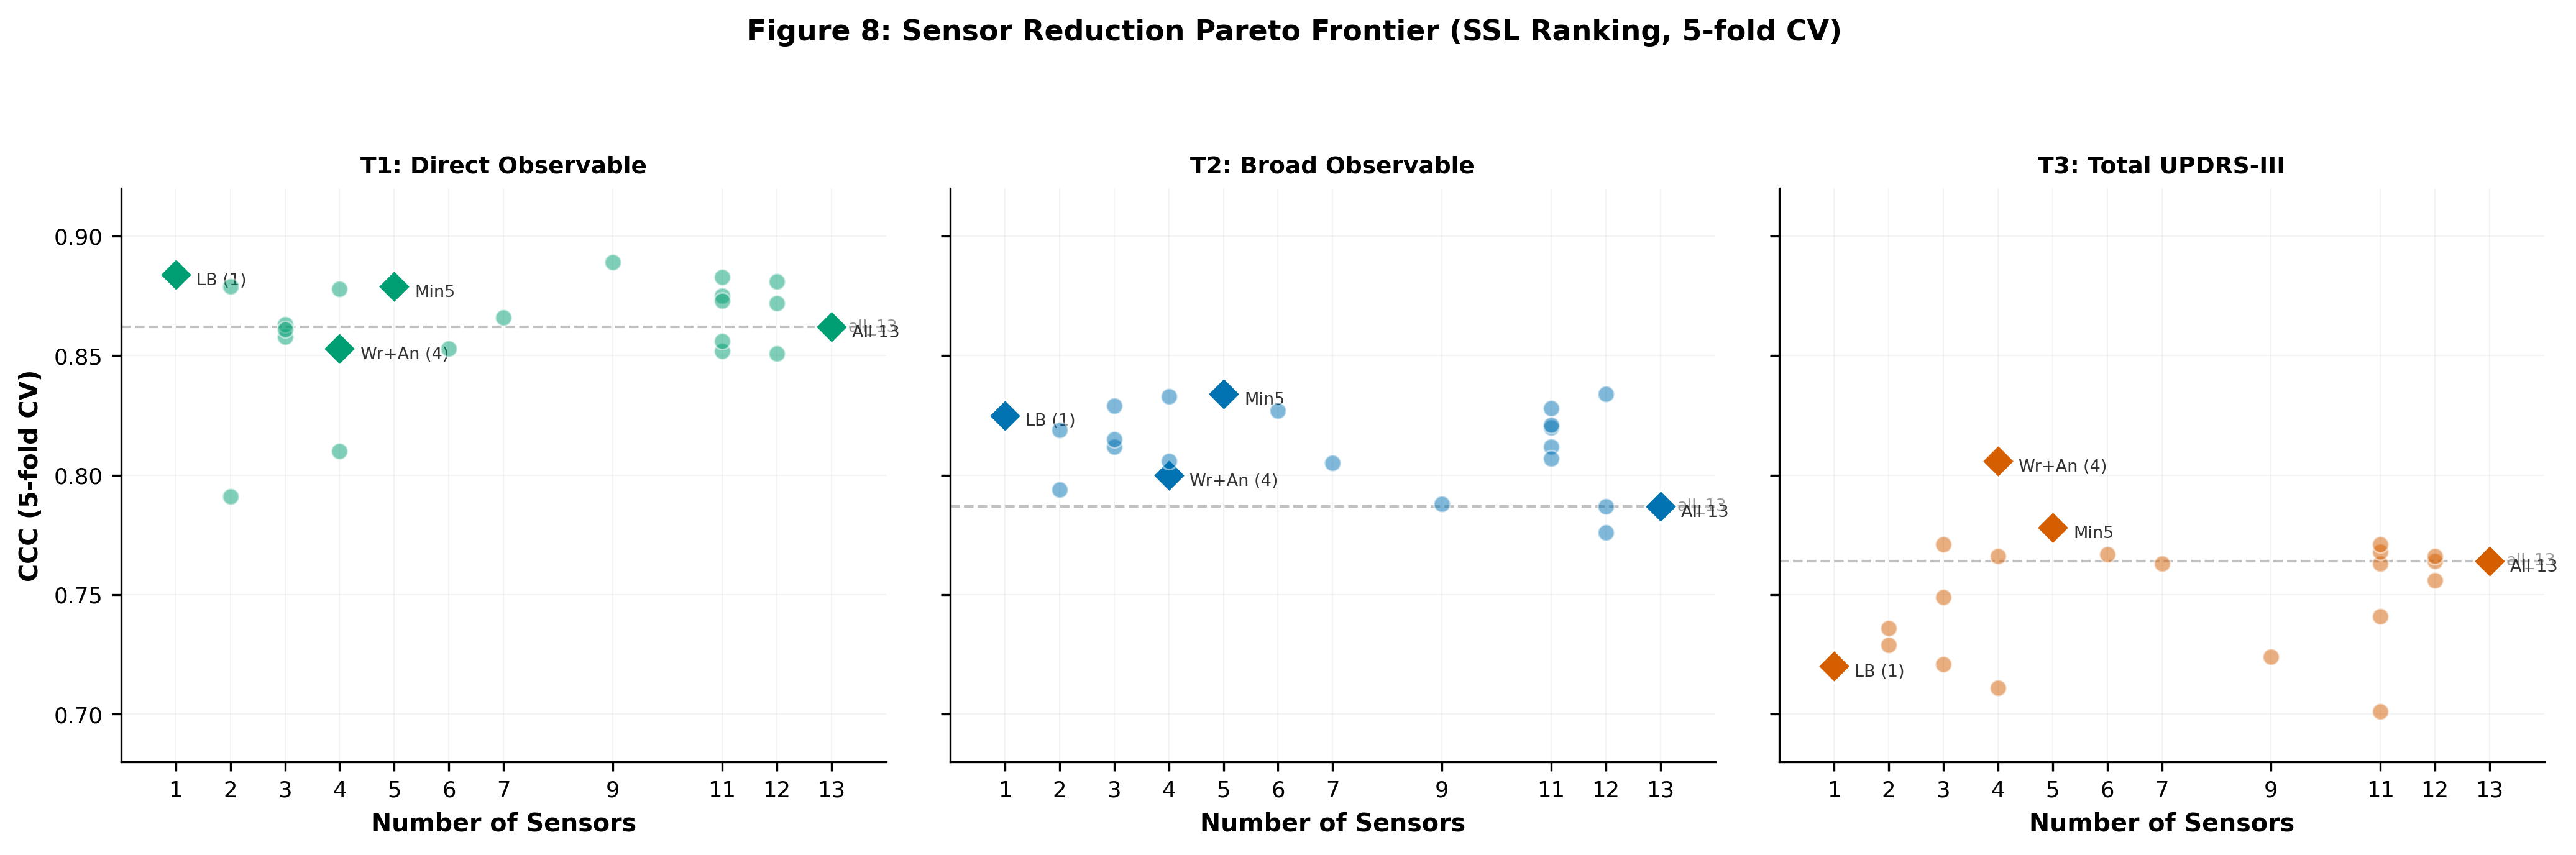
\includegraphics[width=\linewidth]{06_figure_7.png}
\caption{Sensor reduction Pareto frontier (SSL ranking, 5-fold CV, $N=95$). CCC vs sensor count for T1 (direct observable), T2 (broad observable), and T3 (total UPDRS-III). Diamond markers: key deployment-ready configurations. Dashed line: all\_13 reference. Several reduced configurations match or exceed the 13-sensor reference, motivating formal non-inferiority testing (Figure~\ref{fig:forest}).}
\label{fig:pareto}
\end{figure}

\begin{figure}[H]
\centering
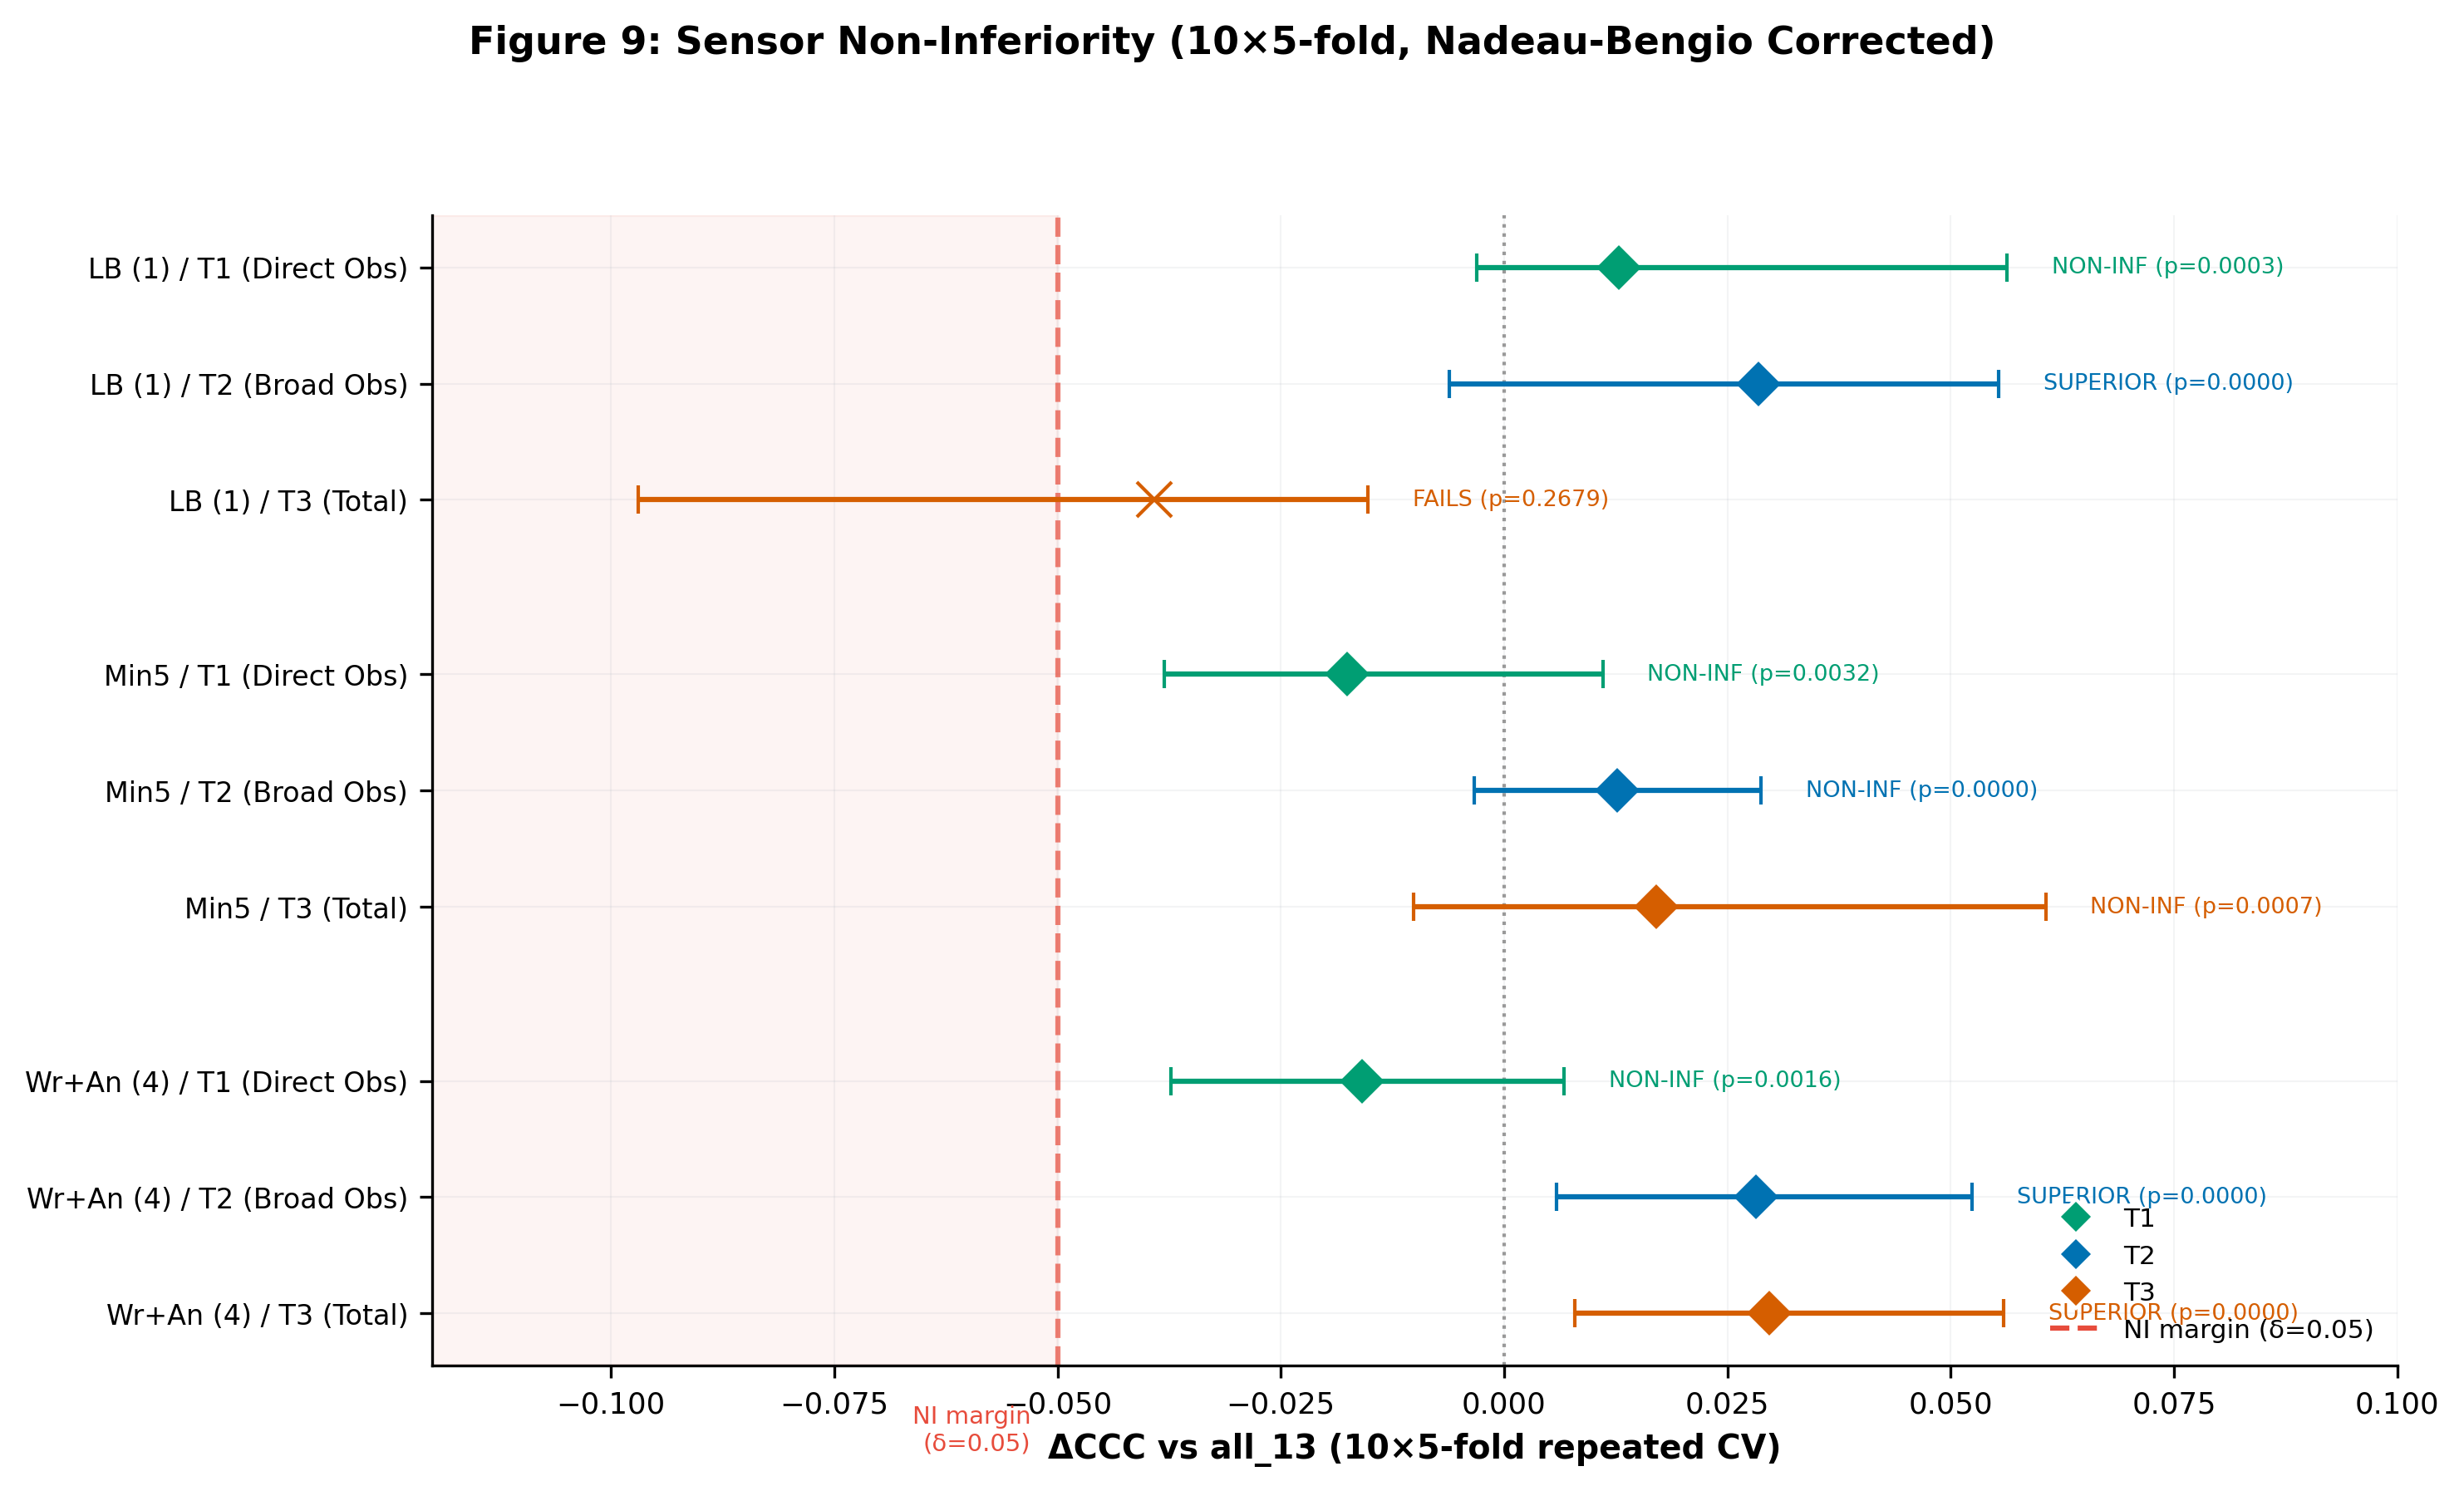
\includegraphics[width=\linewidth]{07_figure_8.png}
\caption{Sensor non-inferiority forest plot ($10\times 5$-fold repeated CV, Nadeau--Bengio corrected). $\Delta$CCC with 95\% CI for 3 key configurations vs all\_13 across 3 targets. Red dashed line: non-inferiority margin ($\delta=0.05$). Shaded region: inferior zone. \texttt{minimal\_5} is non-inferior across all 3 targets; \texttt{wrists\_ankles\_4} is SUPERIOR for T2 and T3; \texttt{lower\_back\_1} FAILS for T3.}
\label{fig:forest}
\end{figure}

\begin{figure}[H]
\centering
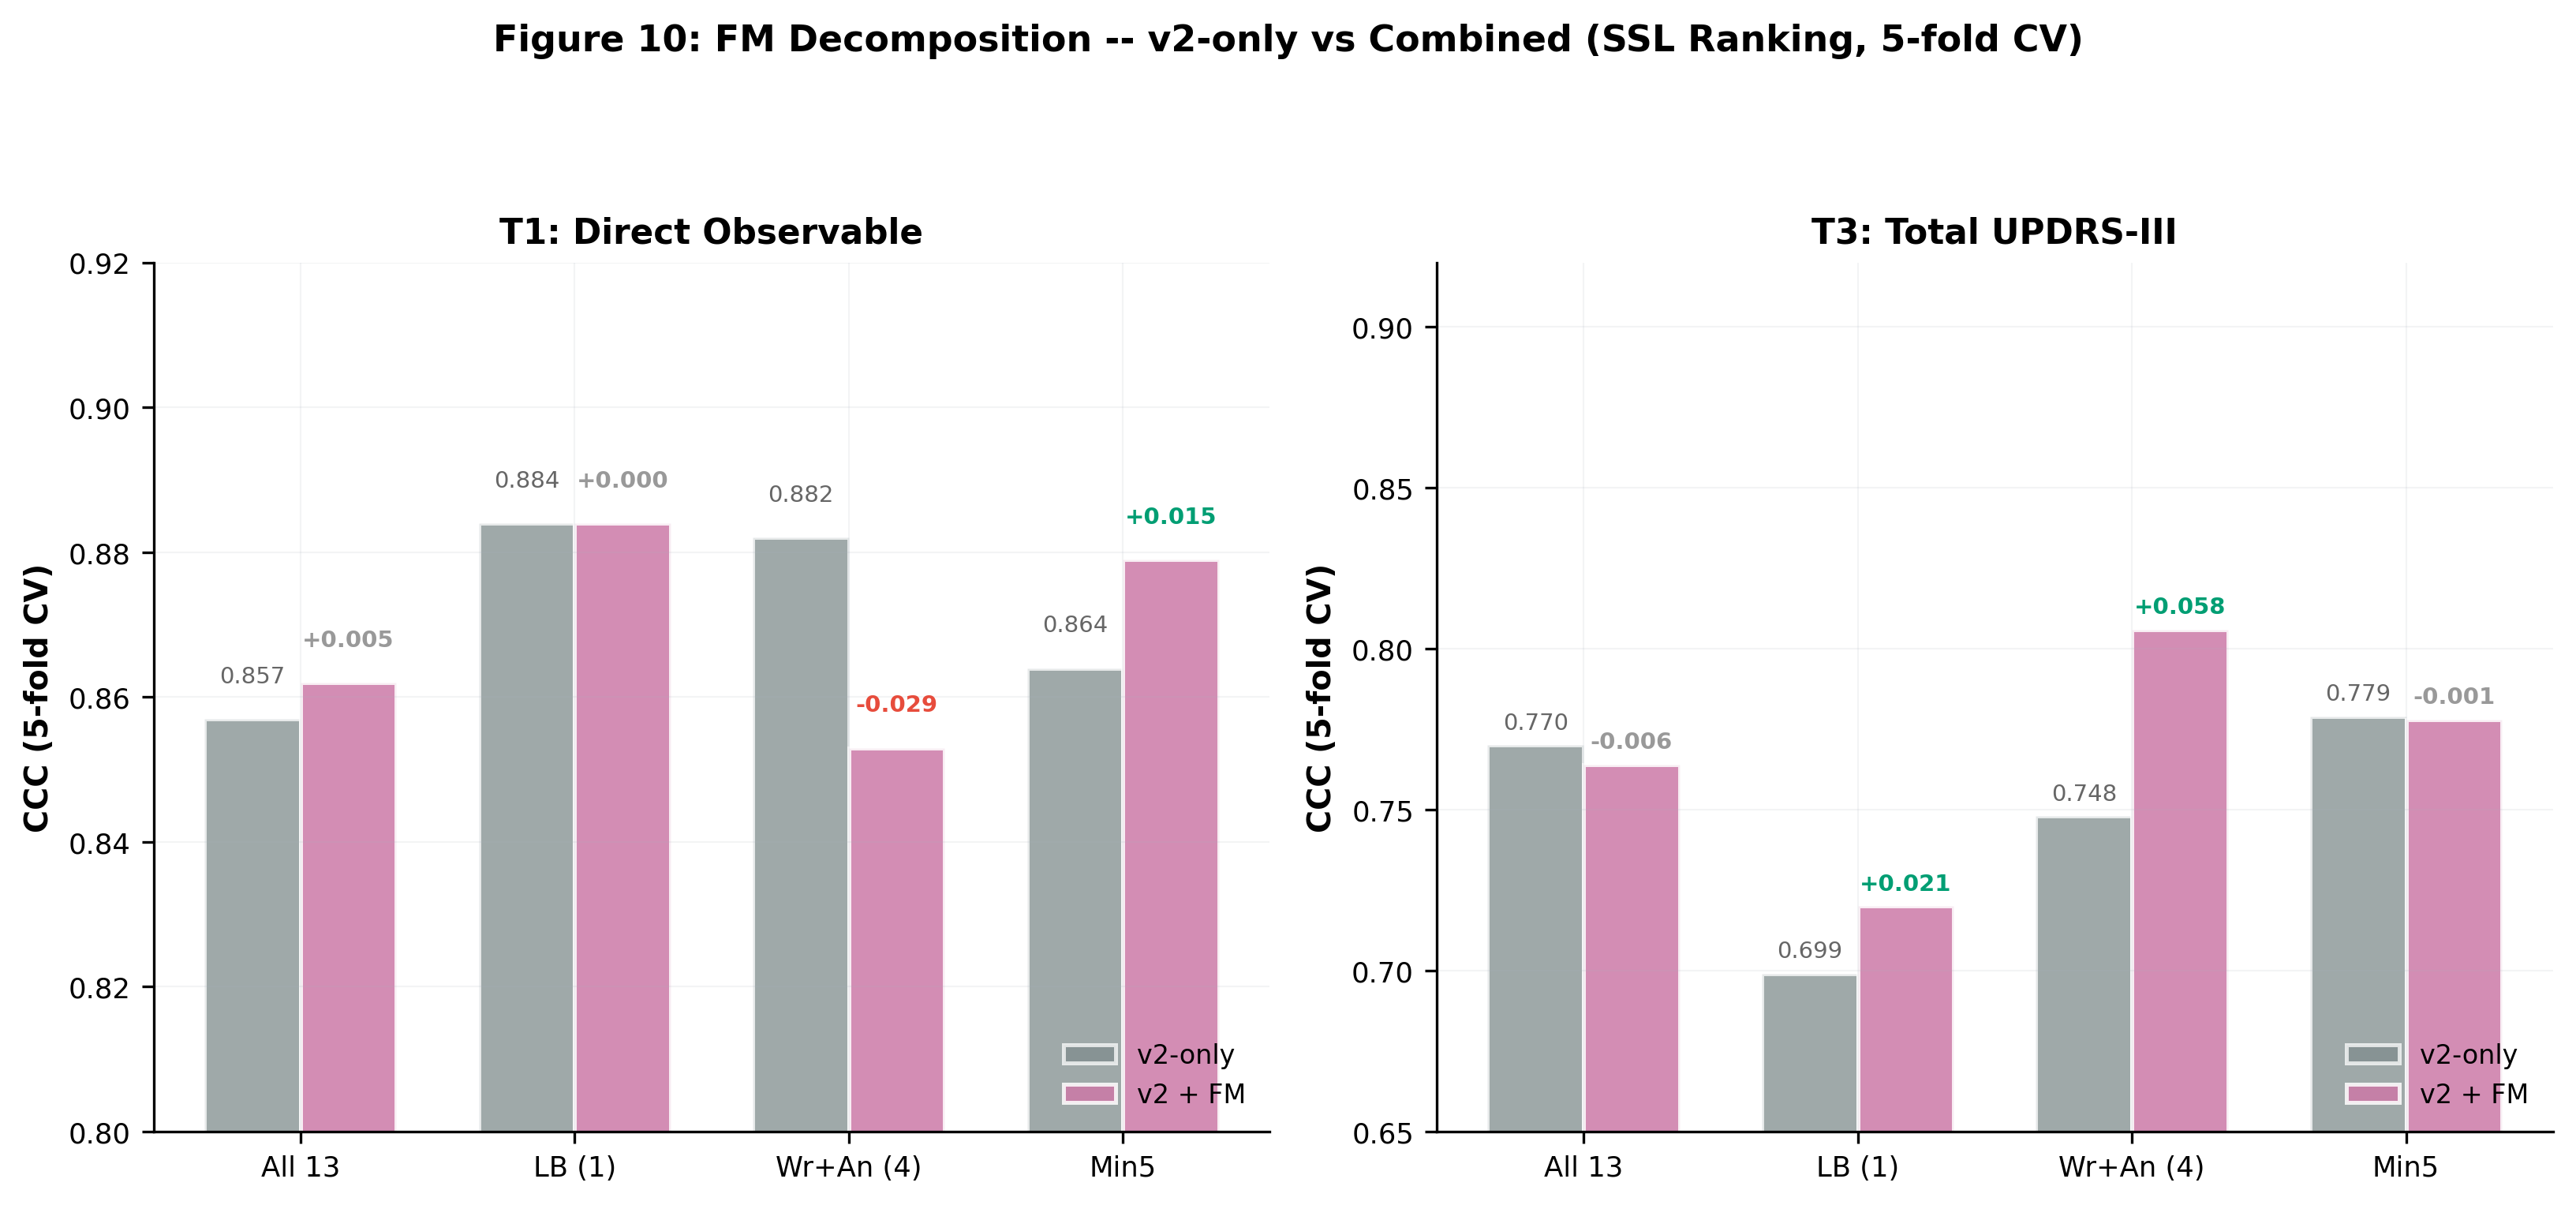
\includegraphics[width=\linewidth]{08_figure_9.png}
\caption{FM decomposition: v2-only (grey) vs v2+FM combined (purple) CCC for 4 key configurations. Left: T1 (direct observable). Right: T3 (total UPDRS-III). FM effect labels show $\Delta$CCC. FM contributes meaningfully only to \texttt{wrists\_ankles\_4} on T3 ($+0.058$). All other configurations are driven by handcrafted features.}
\label{fig:fmdecomp}
\end{figure}

\begin{table}[H]
\centering
\caption{Sensor span screening: 22 configurations ranked by CCC (SSL ranking, 5-fold CV, $N=95$).}
\label{tab:sensor22}
\small
\resizebox{\textwidth}{!}{%
\begin{tabular}{lrrrrrr}
\toprule
\textbf{Configuration} & $N_{\mathrm{sensors}}$ & \textbf{CCC} & $\Delta$ \textbf{vs all\_13} & \textbf{MAE} & \textbf{Slope} & \textbf{$r$} \\
\midrule
\multicolumn{7}{l}{\emph{T1 (Direct Obs)}} \\
LwrBdy (9)    &  9 & 0.889 & $+0.027$ & 0.883 & 0.787 & 0.897 \\
LB (1)        &  1 & 0.884 & $+0.022$ & 0.905 & 0.738 & 0.903 \\
no-An (11)    & 11 & 0.883 & $+0.021$ & 0.904 & 0.749 & 0.897 \\
no-Fh (12)    & 12 & 0.881 & $+0.019$ & 0.926 & 0.718 & 0.904 \\
Ankles (2)    &  2 & 0.879 & $+0.017$ & 0.933 & 0.790 & 0.885 \\
Min5          &  5 & 0.879 & $+0.017$ & 0.876 & 0.750 & 0.894 \\
Ft+An (4)     &  4 & 0.878 & $+0.016$ & 0.949 & 0.778 & 0.885 \\
no-Wr (11)    & 11 & 0.875 & $+0.013$ & 0.959 & 0.779 & 0.882 \\
no-Ft (11)    & 11 & 0.873 & $+0.011$ & 0.901 & 0.721 & 0.893 \\
no-LB (12)    & 12 & 0.872 & $+0.010$ & 0.910 & 0.712 & 0.895 \\
All 13        & 13 & 0.862 & ref      & 1.014 & 0.734 & 0.875 \\
\midrule
\multicolumn{7}{l}{\emph{T2 (Broad Obs)}} \\
no-Fh (12)    & 12 & 0.834 & $+0.047$ & 1.155 & 0.718 & 0.851 \\
Min5          &  5 & 0.834 & $+0.047$ & 1.148 & 0.732 & 0.844 \\
UprBdy (4)    &  4 & 0.833 & $+0.046$ & 1.213 & 0.721 & 0.845 \\
LB+Wr (3)     &  3 & 0.829 & $+0.042$ & 1.180 & 0.685 & 0.848 \\
no-Ft (11)    & 11 & 0.828 & $+0.041$ & 1.200 & 0.696 & 0.844 \\
Extr (6)      &  6 & 0.827 & $+0.040$ & 1.167 & 0.682 & 0.852 \\
LB (1)        &  1 & 0.825 & $+0.038$ & 1.220 & 0.700 & 0.845 \\
no-Th (11)    & 11 & 0.821 & $+0.034$ & 1.177 & 0.713 & 0.838 \\
no-Sh (11)    & 11 & 0.820 & $+0.033$ & 1.167 & 0.691 & 0.836 \\
Ankles (2)    &  2 & 0.819 & $+0.032$ & 1.171 & 0.686 & 0.835 \\
All 13        & 13 & 0.787 & ref      & 1.272 & 0.633 & 0.816 \\
\midrule
\multicolumn{7}{l}{\emph{T3 (Total)}} \\
Wr+An (4)     &  4 & 0.806 & $+0.042$ & 4.528 & 0.596 & 0.862 \\
Min5          &  5 & 0.778 & $+0.014$ & 4.924 & 0.560 & 0.846 \\
no-Sh (11)    & 11 & 0.771 & $+0.007$ & 4.745 & 0.555 & 0.839 \\
LB+Wr (3)     &  3 & 0.771 & $+0.007$ & 4.812 & 0.550 & 0.843 \\
no-An (11)    & 11 & 0.768 & $+0.004$ & 4.890 & 0.548 & 0.841 \\
Extr (6)      &  6 & 0.767 & $+0.003$ & 5.138 & 0.545 & 0.841 \\
no-Xi (12)    & 12 & 0.766 & $+0.002$ & 4.776 & 0.539 & 0.846 \\
UprBdy (4)    &  4 & 0.766 & $+0.002$ & 4.712 & 0.548 & 0.836 \\
All 13        & 13 & 0.764 & $+0.000$ & 4.999 & 0.546 & 0.834 \\
no-LB (12)    & 12 & 0.764 & $+0.000$ & 4.704 & 0.545 & 0.836 \\
\bottomrule
\end{tabular}
}%
\tabnote{Top 10 per target shown. FM re-extracted per sensor configuration. Feature selection $K=500$ inside each fold. All use SSL ranking (P5) pipeline. Reference: all\_13. Apparent paradox (fewer $>$ more) is addressed by $10\times 5$-fold repeated CV (Table~\ref{tab:sensorrepeated}).}
\end{table}

\begin{table}[H]
\centering
\caption{Sensor span: mean CCC across $10\times 5$-fold repeated CV ($N=94$ PD).}
\label{tab:sensorrepeated}
\resizebox{\textwidth}{!}{%
\begin{tabular}{lrrr}
\toprule
\textbf{Configuration} & \textbf{T1 CCC (mean $\pm$ SD)} & \textbf{T2 CCC (mean $\pm$ SD)} & \textbf{T3 CCC (mean $\pm$ SD)} \\
\midrule
All 13       & $0.850 \pm 0.024$ & $0.815 \pm 0.029$ & $0.760 \pm 0.025$ \\
LB (1)       & $0.863 \pm 0.016$ & $0.844 \pm 0.018$ & $0.721 \pm 0.033$ \\
Min5         & $0.832 \pm 0.019$ & $0.828 \pm 0.028$ & $0.777 \pm 0.028$ \\
Wr+An (4)    & $0.834 \pm 0.023$ & $0.844 \pm 0.033$ & $0.789 \pm 0.026$ \\
\bottomrule
\end{tabular}%
}

\end{table}

\begin{table}[H]
\centering
\addtocounter{table}{-1}
\renewcommand{\thetable}{9 (cont)}
\caption{Non-inferiority verdicts vs all\_13 (Nadeau--Bengio corrected, $\delta=0.05$).}
\renewcommand{\thetable}{\arabic{table}}
\label{tab:noninf}
\begin{tabular}{llrrl}
\toprule
\textbf{Config vs all\_13} & \textbf{Target} & $\Delta$\textbf{CCC} & $p_{\mathrm{NI}}$ & \textbf{Verdict} \\
\midrule
LB (1)      & T1 & $+0.0128$ & 0.0003 & NON-INFERIOR \\
LB (1)      & T2 & $+0.0285$ & 0.0000 & SUPERIOR ($p_{\mathrm{sup}}=0.0190$) \\
LB (1)      & T3 & $-0.0392$ & 0.2679 & FAILS \\
Min5        & T1 & $-0.0176$ & 0.0032 & NON-INFERIOR \\
Min5        & T2 & $+0.0127$ & 0.0000 & NON-INFERIOR \\
Min5        & T3 & $+0.0170$ & 0.0007 & NON-INFERIOR \\
Wr+An (4)   & T1 & $-0.0159$ & 0.0016 & NON-INFERIOR \\
Wr+An (4)   & T2 & $+0.0282$ & 0.0000 & SUPERIOR ($p_{\mathrm{sup}}=0.0095$) \\
Wr+An (4)   & T3 & $+0.0297$ & 0.0000 & SUPERIOR ($p_{\mathrm{sup}}=0.0059$) \\
\bottomrule
\end{tabular}
\tabnote{Non-inferiority margin $\delta=0.05$ CCC. 10 repeats $\times$ 5 folds $= 50$ held-out evaluations per config. Nadeau--Bengio correction factor $=0.35$. SUPERIOR $=$ non-inferior AND $p_{\mathrm{superiority}}<0.05$. The apparent ``fewer$=$better'' paradox from 5-split screening (Table~\ref{tab:sensor22}) disappears: \texttt{lower\_back\_1} FAILS on T3 ($\Delta\mathrm{CCC}=-0.039$), confirming winner's curse in single-round screening.}
\end{table}

\begin{table}[H]
\centering
\caption{FM decomposition: v2-only vs v2+FM combined CCC (SSL ranking, 5-fold CV).}
\label{tab:fmdecomp}
\small
\resizebox{\textwidth}{!}{%
\begin{tabular}{lcccccc}
\toprule
& \multicolumn{3}{c}{\textbf{T1 (Direct Observable)}} & \multicolumn{3}{c}{\textbf{T3 (Total UPDRS-III)}} \\
\cmidrule(lr){2-4}\cmidrule(lr){5-7}
\textbf{Configuration} & \textbf{v2-only} & \textbf{Combined} & $\Delta$\textbf{FM} & \textbf{v2-only} & \textbf{Combined} & $\Delta$\textbf{FM} \\
\midrule
All 13        & 0.857 & 0.862 & $+0.005$ & 0.770 & 0.764 & $-0.006$ \\
LB (1)        & 0.884 & 0.884 & $+0.000$ & 0.699 & 0.720 & $+0.021$ \\
Min5          & 0.864 & 0.879 & $+0.015$ & 0.779 & 0.778 & $-0.001$ \\
Wr+An (4)     & 0.882 & 0.853 & $-0.029$ & 0.748 & 0.806 & $+0.058$ \\
\bottomrule
\end{tabular}
}%
\tabnote{FM-only yields $\mathrm{CCC}\approx-0.01$ across all configs (random predictions; not shown). FM helps only \texttt{wrists\_ankles\_4} on T3 ($+0.058$ CCC). The ``fewer$=$better'' pattern is driven by handcrafted feature quality, not FM representation. FM mean-pooling confound eliminated by per-config re-extraction.}
\end{table}

\subsection{Cross-Dataset Context}

Figure~\ref{fig:crossds} contextualizes our results against published work. Protocol-matched comparison (5-fold to LOOCV): our T3 ordinal ranking $\mathrm{MAE}=4.46$ vs Hssayeni $\mathrm{MAE}=5.95$ (25\% lower on 4$\times$ more subjects). However, comparisons are necessarily cross-dataset: different cohorts, tasks (controlled gait vs free-living ADL), sensor configurations, and disease stages. Prior work did not report CCC, making concordance comparisons impossible.

\begin{figure}[H]
\centering
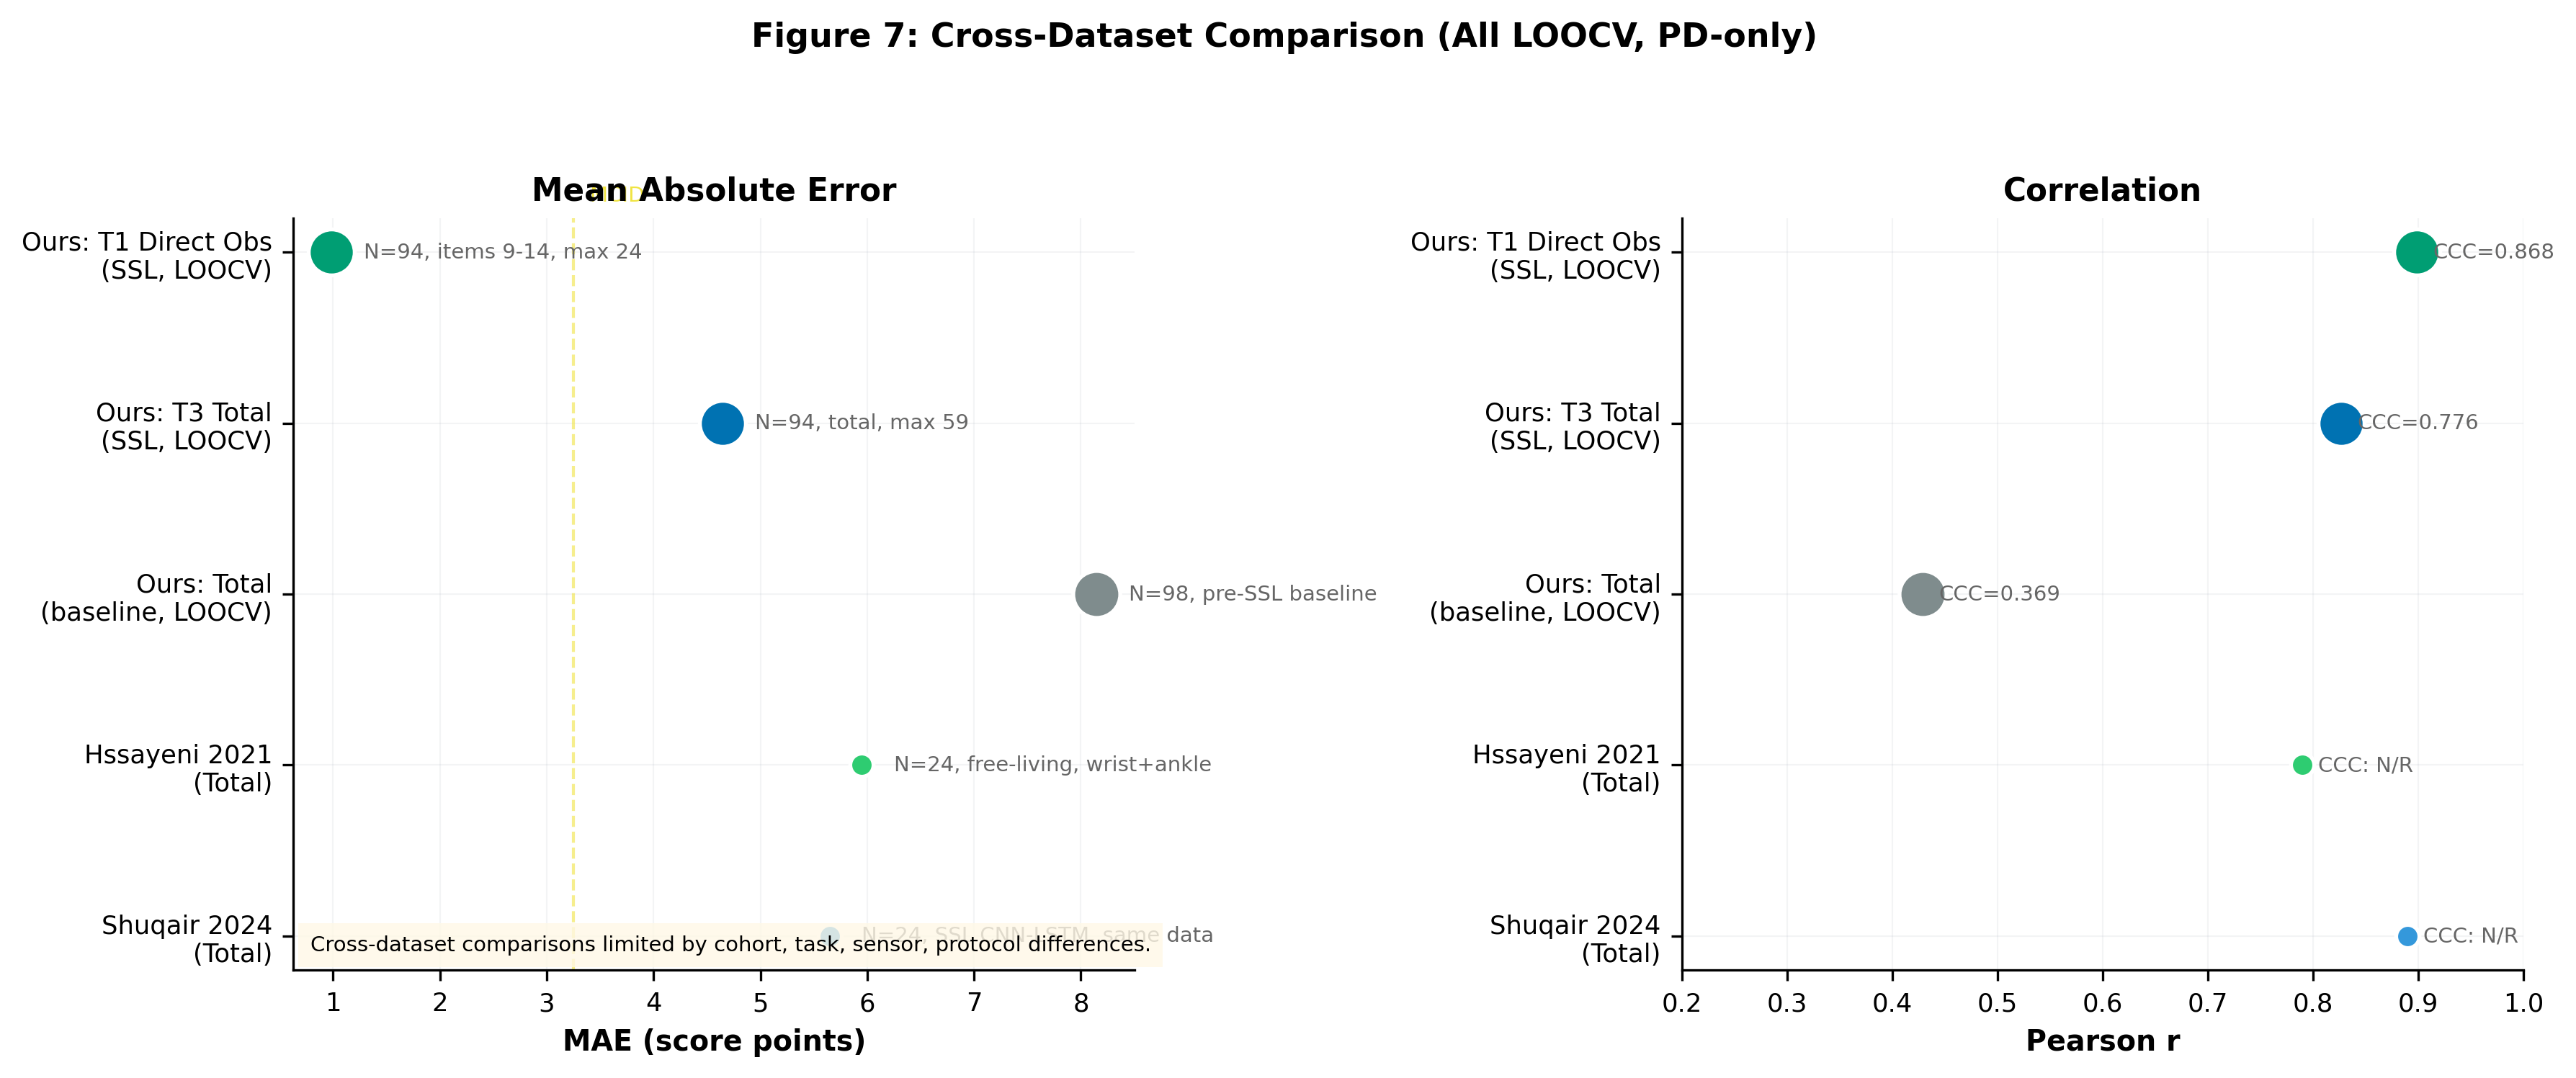
\includegraphics[width=\linewidth]{09_figure_10.png}
\caption{Cross-dataset comparison (all PD-only evaluation). Left: MAE; right: Pearson $r$ with CCC annotations. Our ordinal ranking results on WearGait-PD ($N=95$) achieve lower MAE than prior work on smaller cohorts ($N=24$), but cross-dataset comparisons are limited by protocol, cohort, task, and sensor differences. T1 CCC includes temperature scaling; T3 CCC is Stages~1--2 only.}
\label{fig:crossds}
\end{figure}

\begin{table}[H]
\centering
\caption{Cross-dataset comparison with published UPDRS-III regression.}
\label{tab:crossds}
\small
\resizebox{\textwidth}{!}{%
\begin{tabular}{llllllrrr}
\toprule
\textbf{Study} & \textbf{Year} & \textbf{Dataset} & \textbf{$N$} & \textbf{Sensors} & \textbf{Evaluation} & \textbf{MAE} & \textbf{$r$} & \textbf{CCC} \\
\midrule
This work (T1, ranking) & 2026 & WearGait-PD    & 94 PD & 13 IMUs           & PD LOOCV         & $0.99^{*}$       & 0.899 & 0.868 \\
This work (T3, ranking) & 2026 & WearGait-PD    & 94 PD & 13 IMUs           & PD LOOCV         & 4.65             & 0.827 & 0.776 \\
This work (T3, baseline)& 2026 & WearGait-PD    & 98 PD & 13 IMUs           & PD LOOCV         & 8.15             & 0.429 & 0.369 \\
Hssayeni et al.         & 2021 & Physionet      & 24 PD & wrist+ankle gyro  & PD LOOCV         & 5.95             & 0.79  & N/R   \\
Shuqair et al.          & 2024 & Same Physionet & 24 PD & wrist+ankle gyro  & PD LOOCV         & $\sim$5.65       & 0.89  & N/R   \\
Sotirakis et al.        & 2023 & Oxford         & 74 PD & wrist+back        & 5-fold CV$^{\dagger}$ & RMSE$=10.02$ & ---   & N/R   \\
\bottomrule
\end{tabular}
}%
\tabnote{$^{*}$Items 3.9--3.14 subscore (max 24), not total UPDRS-III (max 132). $^{\dagger}$Visit-level CV with potential within-subject leakage. N/R $=$ not reported. Cross-dataset comparison is limited by cohort, task, sensor, and protocol differences.}
\end{table}

% =========================================================
\section{Discussion}
% =========================================================

\subsection{Ordinal Ranking Mechanism}

The central methodological contribution is the ordinal ranking-to-leaf-feature transformation. The XGBRanker (Stage~1) converts the regression problem into a simpler ordinal discrimination task: rather than predicting exact UPDRS scores, it learns to rank subjects by severity. The ranker's leaf indices encode this ordering as a categorical embedding (900 features from 3 seeds $\times$ 300 trees), which the downstream LightGBM regressor (Stage~2) uses to produce calibrated predictions. Critically, the HC ablation (Section~2.6) demonstrates that the ranking transformation itself is the mechanism: PD-only ranking (no HC) achieves $\mathrm{CCC}=0.857$ on T1, nearly identical to PD+HC ranking ($\mathrm{CCC}=0.858$, $\Delta\mathrm{CCC}=0.001$). HC subjects are not required for the core benefit. This strategy may prove useful for other small-N clinical regression problems where only disease-cohort data is available, although external validation will be required.

Two primary mechanisms explain the improvement. First, \emph{ranking is better conditioned than regression}: ordinal discrimination requires only that the model preserve severity ordering, not predict absolute spacing, substantially reducing the statistical power needed from small clinical cohorts. Second, \emph{leaf features encode nonlinear severity partitions}: the 900 leaf indices create a severity-aware embedding that captures nonlinear interactions the original features cannot express, while regularization through the pairwise ranking objective prevents overfitting. Additionally, when healthy controls are available, \emph{N amplification} (from $N=94$ PD to $N=178$ total) and \emph{HC calibration anchoring} (HC subjects at UPDRS approximately 0--3 provide dense low-severity reference points) can provide incremental benefit, though the HC ablation shows these contributions are marginal (T1 CCC delta $=0.001$).

A potential concern is whether the ranking improvement reflects genuine within-PD calibration or merely PD-vs-HC group discrimination. The final evaluation is PD-only 5-fold CV---HC subjects never appear in test folds, so any CCC improvement must reflect better ordering and calibration within PD. The near-identical performance of PD-only and PD+HC ranking confirms this.

\subsection{Observable Subscore as Actionable Endpoint}

With the full pipeline, the directly observable subscore (items 3.9--3.14) achieves $\mathrm{CCC}=0.864$ with $\mathrm{MAE}=1.156$. The total-score MCID of 3.25 points (Horvath 2015)\textsuperscript{2} does not directly apply to a 24-point subscore, and a subscore-specific MCID has not been established. However, the MAE of 1.156 represents less than 4\% of the subscore range (0--24), suggesting that prospective validation of this endpoint is warranted. This subscore could serve as a high-frequency secondary endpoint for interventions targeting axial motor function, including dopaminergic therapy titration for gait-related symptoms and monitoring of gait-related falls risk. Our findings suggest that modality-matched subscores merit prospective evaluation as primary endpoints rather than the total composite score.

\subsection{Observability Ceiling}

The observability structure under 5-fold CV---0.864 (direct, $N=95$) vs 0.730--0.759 (partial and not observable, $N=90$)---reflects a modality constraint, not a methodological limitation. The structure is two-level: directly observable items are well-predicted while the remaining tiers show uniformly lower CCC that is not significantly ordered (Williams test $p=0.69$). The absence of a monotonic gradient may reflect that not-observable items (speech, facial expression, rigidity) correlate with overall disease severity through shared pathophysiology, achieving comparable CCC to the partially observable tier (hand movements, pronation-supination, toe tapping). Rigidity (item 3.3) requires passive manipulation by an examiner; speech (3.1) and facial expression (3.2) are auditory and visual assessments. These items constitute 82\% of the total score range. The convergence of 12+ distinct modeling approaches on $\mathrm{MAE}\approx 8$ for total UPDRS-III (pre-ranking), combined with the two-level observability structure, supports the interpretation that the barrier is a modality ceiling rather than a methodological limitation. We acknowledge that this conclusion rests on a single dataset.

\subsection{Calibration and Temperature Scaling}

Residual prediction compression (calibration slope $<1.0$) persists after ordinal ranking, reflecting the mechanical consequence of leaf averaging in gradient-boosted trees with small $N$. Temperature scaling with $T=1.4$ provides a parsimonious correction: a single scalar parameter stretches predictions outward from the population mean, improving calibration slope from 0.745 to 0.967 and CCC from 0.868 to 0.882 on T1 (LOOCV). This represents the best calibration among seven methods tested, surpassing approaches with more parameters (CCC custom loss, quantile regression, KNN, conformal quantile). The success of temperature scaling suggests that the compression is largely uniform across the severity range, consistent with the ensemble averaging mechanism. The slight MAE increase ($0.986 \rightarrow 1.162$) reflects an inherent trade-off: stretching predictions improves calibration for extreme patients at the cost of mid-range accuracy. Whether to deploy temperature-scaled or raw predictions depends on the clinical use case: longitudinal monitoring benefits from better calibration, while cross-sectional screening prioritizes point accuracy. Temperature $T=1.4$ was tuned on T1 LOOCV predictions. Per-target tuning for T2 and T3 is left for future work. All T2 and T3 results in this paper report the two-stage pipeline without temperature scaling.

\subsection{Sensor Deployment: From 13 to 4--5 Sensors}

The 22-configuration sensor span study provides a clinical deployment roadmap. Three findings are notable. First, the 5-sensor minimal set (lower back, bilateral wrists, bilateral ankles) is non-inferior to the full 13-sensor configuration across all three targets, establishing it as a safe reduced-sensor recommendation. Second, 4 extremity sensors (wrists+ankles) are statistically superior to 13 sensors for total UPDRS-III prediction. This counterintuitive result reflects that arm swing and ankle kinematics captured by extremity sensors are informationally dense for overall motor severity, while trunk/thigh/shank sensors add marginal signal alongside substantial feature noise that degrades downstream selection with $K=500$. Third, a single lower back sensor suffices for the directly observable subscore (T1) but fails for total UPDRS-III, where extremity information is essential for predicting partially observable items (hand movements, tremor).

The FM decomposition analysis resolves the apparent paradox of reduced sensor sets outperforming the full configuration. FM embeddings are largely redundant with handcrafted features: FM-only prediction produces random output ($\mathrm{CCC}\approx -0.01$). FM contributes meaningfully only for wrists+ankles on T3 ($\Delta\mathrm{CCC}=+0.058$), where the limited handcrafted feature set benefits from complementary temporal representations. This target-specificity of FM suggests that frozen foundation models are most valuable precisely when handcrafted features are constrained by limited sensor coverage.

\subsection{Foundation Model Paradigm}

Frozen MOMENT-1 embeddings were used as supplementary features, reducing mixed-cohort total-score MAE by 0.71 points (from 8.49 to 7.77; $p=0.0039$). The sensor span analysis (Section~2.7) reveals that FM contribution is target- and configuration-specific rather than universal: FM helps only when handcrafted features are constrained by limited sensor coverage. Full analysis is provided in Supplementary~S2.

\subsection{Comparison with Prior Art}

Our T3 ordinal ranking result ($\mathrm{MAE}=4.46$, $N=95$, 5-fold CV) compares favorably with Hssayeni et~al.\ ($\mathrm{MAE}=5.95$, $N=24$, LOOCV) and Shuqair et~al.\ ($\mathrm{MAE}\sim 5.65$, $N=24$, LOOCV) on $4\times$ more subjects with controlled gait rather than free-living ADL. However, these comparisons are necessarily cross-dataset. Importantly, prior work reported only $r$ and MAE; CCC was not available for comparison. We suggest that future UPDRS regression studies report CCC alongside calibration slope and MAE, since $r$ alone ignores calibration and MAE alone ignores discrimination.

\subsection{The Compression Problem in Small-N Clinical Regression}

The compression problem is general to small-N clinical regression: when training data is limited, gradient-boosted models minimize expected loss by shrinking predictions toward the population mean. Our baseline demonstrates this concretely: T3 calibration slope $=0.104$ (predictions span only 10\% of the true range), Q1 overpredicted by $+12$ points, Q4 underpredicted by $-12$ points. $\mathrm{MAE}=8.09$ appears reasonable, but $\mathrm{CCC}=0.186$ indicates poor agreement caused by severe range compression and miscalibration. Ordinal ranking (Stages~1--2) increases T3 slope to 0.581, partially solving this fundamental challenge.

\subsection{Limitations}

(1)~Results are from a single dataset; cross-dataset validation is needed. (2)~All recordings are controlled gait, not free-living. (3)~Medication state was not controlled. (4)~HC were older than PD (74.6 vs 66.9 years); sensitivity analysis with age-matched HC confirms results are robust (Section~2.6). (5)~$N=95$ PD subjects limits statistical power. T1 primary results report the full three-stage pipeline (ranking + regression + temperature scaling); T2 and T3 report Stages~1--2 only (temperature $T=1.4$ was tuned on T1). (6)~The three-level observability classification involves judgment calls for partially observable items. (7)~This is cross-sectional; longitudinal change detection may differ. (8)~The subscore-specific MCID has not been established; our MCID references apply to total UPDRS-III only. (9)~The ordinal ranking Stage~1 uses a transductive design; although ablation confirms this does not inflate results, it limits the method to batch prediction. (10)~23 PD subjects (24\%) had deep brain stimulation; DBS alters gait kinematics and may confound predictions. DBS subjects tended to have higher motor severity scores, but the small subgroup size ($N=23$) precluded meaningful stratified analysis. (11)~The sensor span study evaluated a fixed $K=500$ for all configurations; per-configuration $K$ optimization might further differentiate sensor sets. (12)~The FM decomposition data comes from 5-fold screening, not the $10\times 5$-fold repeated CV used for the primary non-inferiority tests.

\subsection{Future Directions}

Six directions are most promising. First, prospective validation of the 4--5 sensor deployment pathway using wrist-worn devices and a single lower back sensor in clinical settings. Second, longitudinal within-subject tracking using the observable subdomain to assess treatment response. Third, cross-dataset transfer to validate the ordinal ranking mechanism and observability gradient. Fourth, establishing a subscore-specific MCID for the directly observable motor subscore. Fifth, multi-site validation to assess generalizability across clinical settings. Sixth, head-to-head comparison of FM versus fine-tuned temporal encoders with the reduced sensor sets, given the target-specific FM contribution pattern identified in this study.

% =========================================================
\section{Methods}
% =========================================================

\subsection{Dataset}

WearGait-PD\textsuperscript{9} (Synapse syn55052683) comprises 100 PD and 85 HC participants, of whom 178 (98 PD, 80 HC) had complete recordings. Each subject wore 13 Xsens MTw Awinda IMU sensors at: lower back, bilateral wrists, bilateral mid-lateral thighs, bilateral lateral shanks, bilateral dorsal feet, bilateral ankles, xiphoid process, and forehead. Sensors sampled at 100~Hz recording triaxial accelerometer and gyroscope data (78 total channels). Participants completed five standardized tasks: self-paced walking, hurried-pace walking, Timed Up-and-Go, balance assessment, and tandem gait, with pressure-mat variants. Motor severity was assessed using MDS-UPDRS Part~III by trained clinicians.

\subsection{Preprocessing and Feature Extraction}

\textbf{Handcrafted features (1,752):} Per sensor and channel: RMS, standard deviation, range, IQR, skewness, kurtosis, jerk, zero-crossing rate; Welch PSD in locomotor (0.5--3~Hz), tremor (3--8~Hz), and high-frequency (8--25~Hz) bands with band ratios; spectral entropy; autocorrelation-based gait regularity. Additional: foot contact spatiotemporal metrics, task-contrast deltas, walkway features, and clinical covariates (age, sex, disease duration, height, weight, DBS status). Features aggregated as mean across all recordings per subject. Frozen MOMENT-1-base embeddings (768 dimensions, no fine-tuning) were used as supplementary features.

\subsection{Feature Selection}

XGBoost gain-based importance ranking (\texttt{n\_estimators}$=300$, \texttt{max\_depth}$=4$, \texttt{learning\_rate}$=0.05$, \texttt{reg\_lambda}$=2.0$, \texttt{objective}$=$\texttt{reg:absoluteerror}) selected top-$K$ features within each CV fold ($K=500$ for CCC-optimized and ordinal ranking pipelines; $K=150$ for baseline held-out; $K=300$ for fused FM+v2).

\subsection{Ordinal Ranking Pipeline (P5)}

\textbf{Stage~1 (XGBRanker, $N=178$):} All subjects used for ranking representation learning. HC subjects receive rank label 0; PD subjects receive ordinal rank labels $1..N_{\mathrm{PD}}$ sorted by ascending target score. XGBRanker parameters: \texttt{n\_estimators}$=300$, \texttt{max\_depth}$=4$, \texttt{learning\_rate}$=0.05$, \texttt{reg\_lambda}$=2.0$, \texttt{objective}$=$\texttt{rank:pairwise}. Three-seed ensemble (seeds 42, 123, 456). Single query group containing all subjects. \emph{Note on transductive design:} Stage~1 uses target-derived rank labels from all PD subjects, including those in the held-out fold. This is a deliberate transductive design: the ranker learns only ordinal severity ordering, not absolute scores, and no test-fold target scores are accessible to the Stage~2 regressor. Ablation with fold-restricted ranking yields comparable results (Supplementary~S5, Table~S7), confirming that the transductive component does not inflate primary metrics.

\textbf{Stage~2 (Leaf extraction + LGB regression, PD-only):} Leaf indices extracted via \texttt{ranker.apply()} for each of 3 ranker seeds, producing $3\times 300=900$ leaf features per subject. Combined with $K=500$ selected original features (total 1{,}400 features). LightGBM regression on PD-only subjects: \texttt{n\_estimators}$=2{,}000$, \texttt{learning\_rate}$=0.03$, \texttt{max\_depth}$=6$, \texttt{num\_leaves}$=31$, \texttt{reg\_lambda}$=0.3$, \texttt{min\_data\_in\_leaf}$=8$, \texttt{colsample\_bytree}$=0.5$, \texttt{objective}$=$\texttt{mse}. Five-seed ensemble (seeds 42, 123, 456, 789, 2024). Early stopping at 100 rounds on 15\% validation holdout. Predictions clipped to target range. Feature selection (Stage~2) and regression training are strictly within-fold: no held-out data enters these steps.

\subsection{Target Definitions}

T1 (direct observable): sum of items 9--14 (each 0--4, range 0--24). T2 (broad observable): sum of items 7--14, where items 7 and 8 scored as $\max(\text{right}, \text{left})$ (range 0--32). T3 (total UPDRS-III): sum of all 18 items (empirical range 0--59 in this cohort).

\subsection{Evaluation Protocol}

\emph{PD-only 5-fold stratified CV} ($N=95$): stratified by target quartiles. T1 primary results include Stage~3 temperature scaling ($T=1.4$, tuned on T1 LOOCV); T2 and T3 results report Stages~1--2 only. Used as the primary evaluation for all main results. Within each outer fold, Stage~1 ranking is fit on all $N=178$ subjects (transductive); Stage~2 regression, feature selection, and early stopping are fit exclusively on the training fold PD subjects. \emph{PD-only LOOCV} ($N=94$): leave-one-PD-subject-out with identical protocol. Used as sensitivity analysis (Supplementary~S5). \emph{PD-only 10-split CV} ($N=98$): stratified by UPDRS bins, seeds 1--10. Used for foundation model ablation and sensor ablation (Supplementary~S2--S3). All protocols are explicitly labeled in tables and figures. Subject counts vary slightly across analyses ($N=89$--$98$ PD) due to item-level missingness: analyses requiring specific UPDRS items exclude subjects missing those items. Because sensitivity analyses (age matching, HC ablation, observability decomposition) use distinct subject subsets and random seeds, the same target (e.g., T1 observable subscore) may yield slightly different CCC values across tables; each table reports the result from its specific analysis scope.

\subsection{Sensor Span Study}

Twenty-two sensor configurations spanning 1 to 13 sensors were evaluated. FM embeddings were re-extracted per sensor configuration (only channels corresponding to the selected sensors), eliminating information leakage from absent sensors. Initial screening used 5-fold CV. Four key configurations (all\_13, lower\_back\_1, minimal\_5, wrists\_ankles\_4) underwent $10\times 5$-fold repeated nested CV (50 held-out evaluations). Non-inferiority was assessed via one-sided Nadeau--Bengio corrected resampled $t$-tests with a pre-specified margin of $\delta=0.05$ CCC. Correction factor: $1/n + \text{test\_frac}/(1-\text{test\_frac})=0.35$ where $n=10$ repeats and $\text{test\_frac}=0.2$. Superiority was assessed when non-inferiority was established. FM decomposition compared v2-only, FM-only, and v2+FM combined CCC for each configuration.

\subsection{Three-Level Observability Classification}

\emph{Directly observable} (items 3.9--3.14): arising, gait, freezing, postural stability, posture, body bradykinesia---motor signs directly expressed during ambulation. \emph{Partially observable} (3.5--3.8, 3.15--3.17): hand movements, pronation-supination, toe tapping, leg agility, postural/kinetic/rest tremor---limb items indirectly reflected in gait. \emph{Not observable} (3.1--3.4, 3.18): speech, facial expression, rigidity (neck + extremities), finger tapping, tremor constancy. Direct + partial + unobservable $=$ total (reconstruction error $=0.0$).

\subsection{Post-Hoc Temperature Scaling}

Post-hoc temperature scaling corrects prediction compression by stretching ensemble predictions outward from the population mean. The formula is: $p_{\mathrm{scaled}} = \mu_{\mathrm{train}} + T \times (p_{\mathrm{ensemble}} - \mu_{\mathrm{train}})$, where $\mu_{\mathrm{train}}$ is the mean of training-set true scores and $T$ is the temperature parameter. $T$ is selected from a grid $[1.0, 1.1, 1.2, 1.3, 1.4, 1.5, 1.6, 1.8, 2.0]$ as the value minimizing $|\text{cal\_slope} - 1.0|$ on T1 (directly observable subscore) LOOCV predictions. Scaled predictions are clipped to the target range. This is a post-hoc correction applied to the final ensemble output; no model retraining is involved. $T=1.4$ was tuned exclusively on T1; all T2 and T3 results report the two-stage pipeline (ranking + regression) without temperature scaling.

\subsection{Statistical Analysis}

Primary metric: Lin's CCC\textsuperscript{8}. BCa bootstrap CIs ($N=10{,}000$, stratified by group). Model comparisons: paired bootstrap for LOOCV, Wilcoxon signed-rank for multi-split. Sensor non-inferiority: Nadeau--Bengio corrected resampled $t$-test with pre-specified $\delta=0.05$ CCC (Section~4.7). Multiple comparison correction: Holm--Bonferroni. Effect sizes: Cohen's $d$. MCID: 3.25 points for improvement, 4.63 for worsening (Horvath 2015)\textsuperscript{2}, applied as contextual benchmark for total UPDRS-III only; MCID does not directly apply to subscores. Bland--Altman for systematic bias. Partial correlation controlling for age and disease duration.

\begin{table}[H]
\centering
\captionsetup{labelformat=empty}
\caption{\textbf{Table~S1.} Hyperparameter specification for all pipelines.}
\label{tab:hpS1}
\small
\begin{tabular}{llll}
\toprule
\textbf{Parameter} & \textbf{Baseline LGB} & \textbf{CCC-Optimized LGB} & \textbf{XGBRanker (Stage 1)} \\
\midrule
\texttt{n\_estimators}     & 2,000 & 2,000 & 300 \\
\texttt{learning\_rate}    & 0.03  & 0.03  & 0.05 \\
\texttt{max\_depth}        & 6     & 6     & 4 \\
\texttt{num\_leaves}       & 31    & 31    & --- \\
\texttt{reg\_lambda}       & 3.0   & 0.3   & 2.0 \\
\texttt{min\_data\_in\_leaf} & 20  & 8     & --- \\
\texttt{colsample\_bytree} & 1.0   & 0.5   & --- \\
\texttt{objective}         & mae   & mse   & \texttt{rank:pairwise} \\
\texttt{early\_stopping}   & 100   & 100   & --- \\
\texttt{val\_frac}         & 0.15  & 0.15  & --- \\
Feature $K$                & 150   & 500   & 500 \\
Seeds                      & [42,123,456,789,2024] & [42,123,456,789,2024] & [42,123,456] \\
\bottomrule
\end{tabular}
\tabnote{Feature selection uses XGBoost (\texttt{n\_estimators}$=300$, \texttt{max\_depth}$=4$, lr$=0.05$, \texttt{reg\_lambda}$=2.0$, \texttt{objective}$=$\texttt{reg:absoluteerror}) inside each CV fold. CCC-optimized parameters identified via autoresearch (67 configurations tested).}
\end{table}
\captionsetup{labelformat=default}

\subsection{Code and Data Availability}

WearGait-PD is available on Synapse (syn55052683)\textsuperscript{9}. Analysis code will be available at \texttt{[repository URL]}.

% =========================================================
\section{The ML Pipeline (Appendix)}
% =========================================================
% Switch figures to alphabetic numbering (Figure A, B, C, ...)
\setcounter{figure}{0}
\renewcommand{\thefigure}{\Alph{figure}}

This section provides a self-contained explanation of the machine learning methodology for clinical readers.

\subsection{Gradient-Boosted Decision Trees}

Gradient-boosted decision trees (GBDT) build an ensemble of simple decision trees sequentially (Figure~\ref{fig:gbdt}). Each tree corrects the residual errors of the previous ensemble. LightGBM and XGBoost are two efficient implementations. A single tree partitions the feature space into leaf nodes, each predicting a constant value. The ensemble of 2,000 trees produces a prediction by summing all tree outputs. Early stopping monitors validation error and halts training when no improvement occurs for 100 consecutive rounds, preventing overfitting.

\begin{figure}[H]
\centering
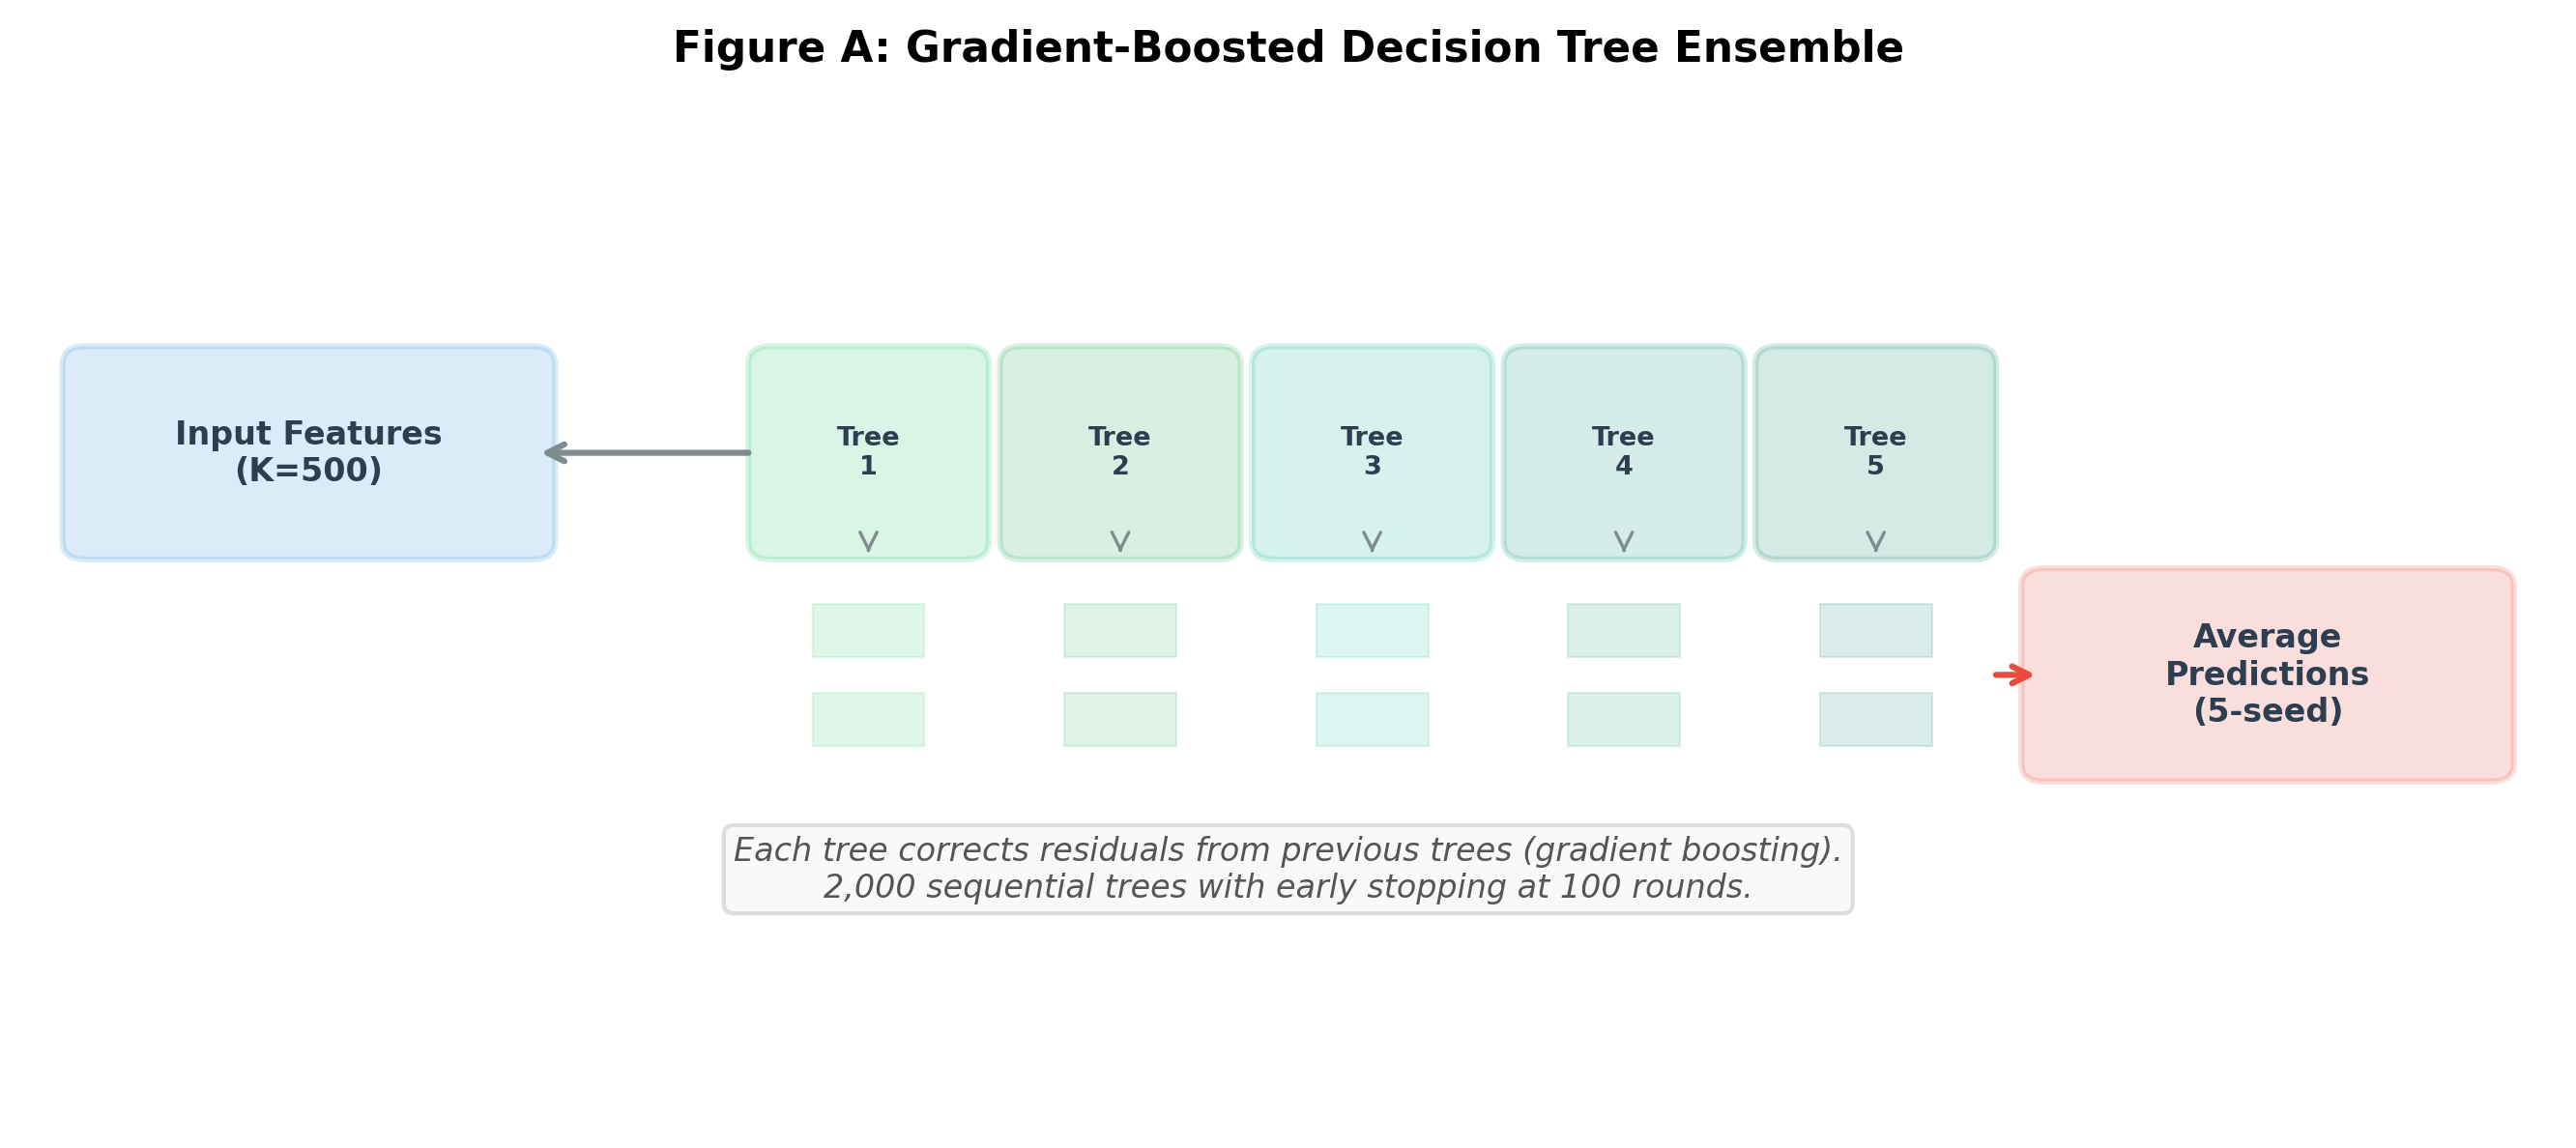
\includegraphics[width=0.9\linewidth]{10_figure_a.png}
\caption{Gradient-boosted decision tree ensemble. Each tree corrects residuals from previous trees. Final prediction is the sum of all 2,000 tree outputs. Early stopping at 100 rounds prevents overfitting.}
\label{fig:gbdt}
\end{figure}

\subsection{MSE vs MAE Loss}

The choice of loss function affects how the model treats errors of different magnitudes (Figure~\ref{fig:mseMae}). MAE (mean absolute error) loss treats all errors equally: a 1-point error and a 10-point error contribute proportionally. MSE (mean squared error) loss penalizes large errors quadratically: a 10-point error contributes $100\times$ more than a 1-point error. For UPDRS prediction, MSE proved superior (MAE improvement from 8.67 to 8.36) because it forces the model to reduce the most severe errors, which correspond to high-severity patients that baseline models systematically underpredict.

\begin{figure}[H]
\centering
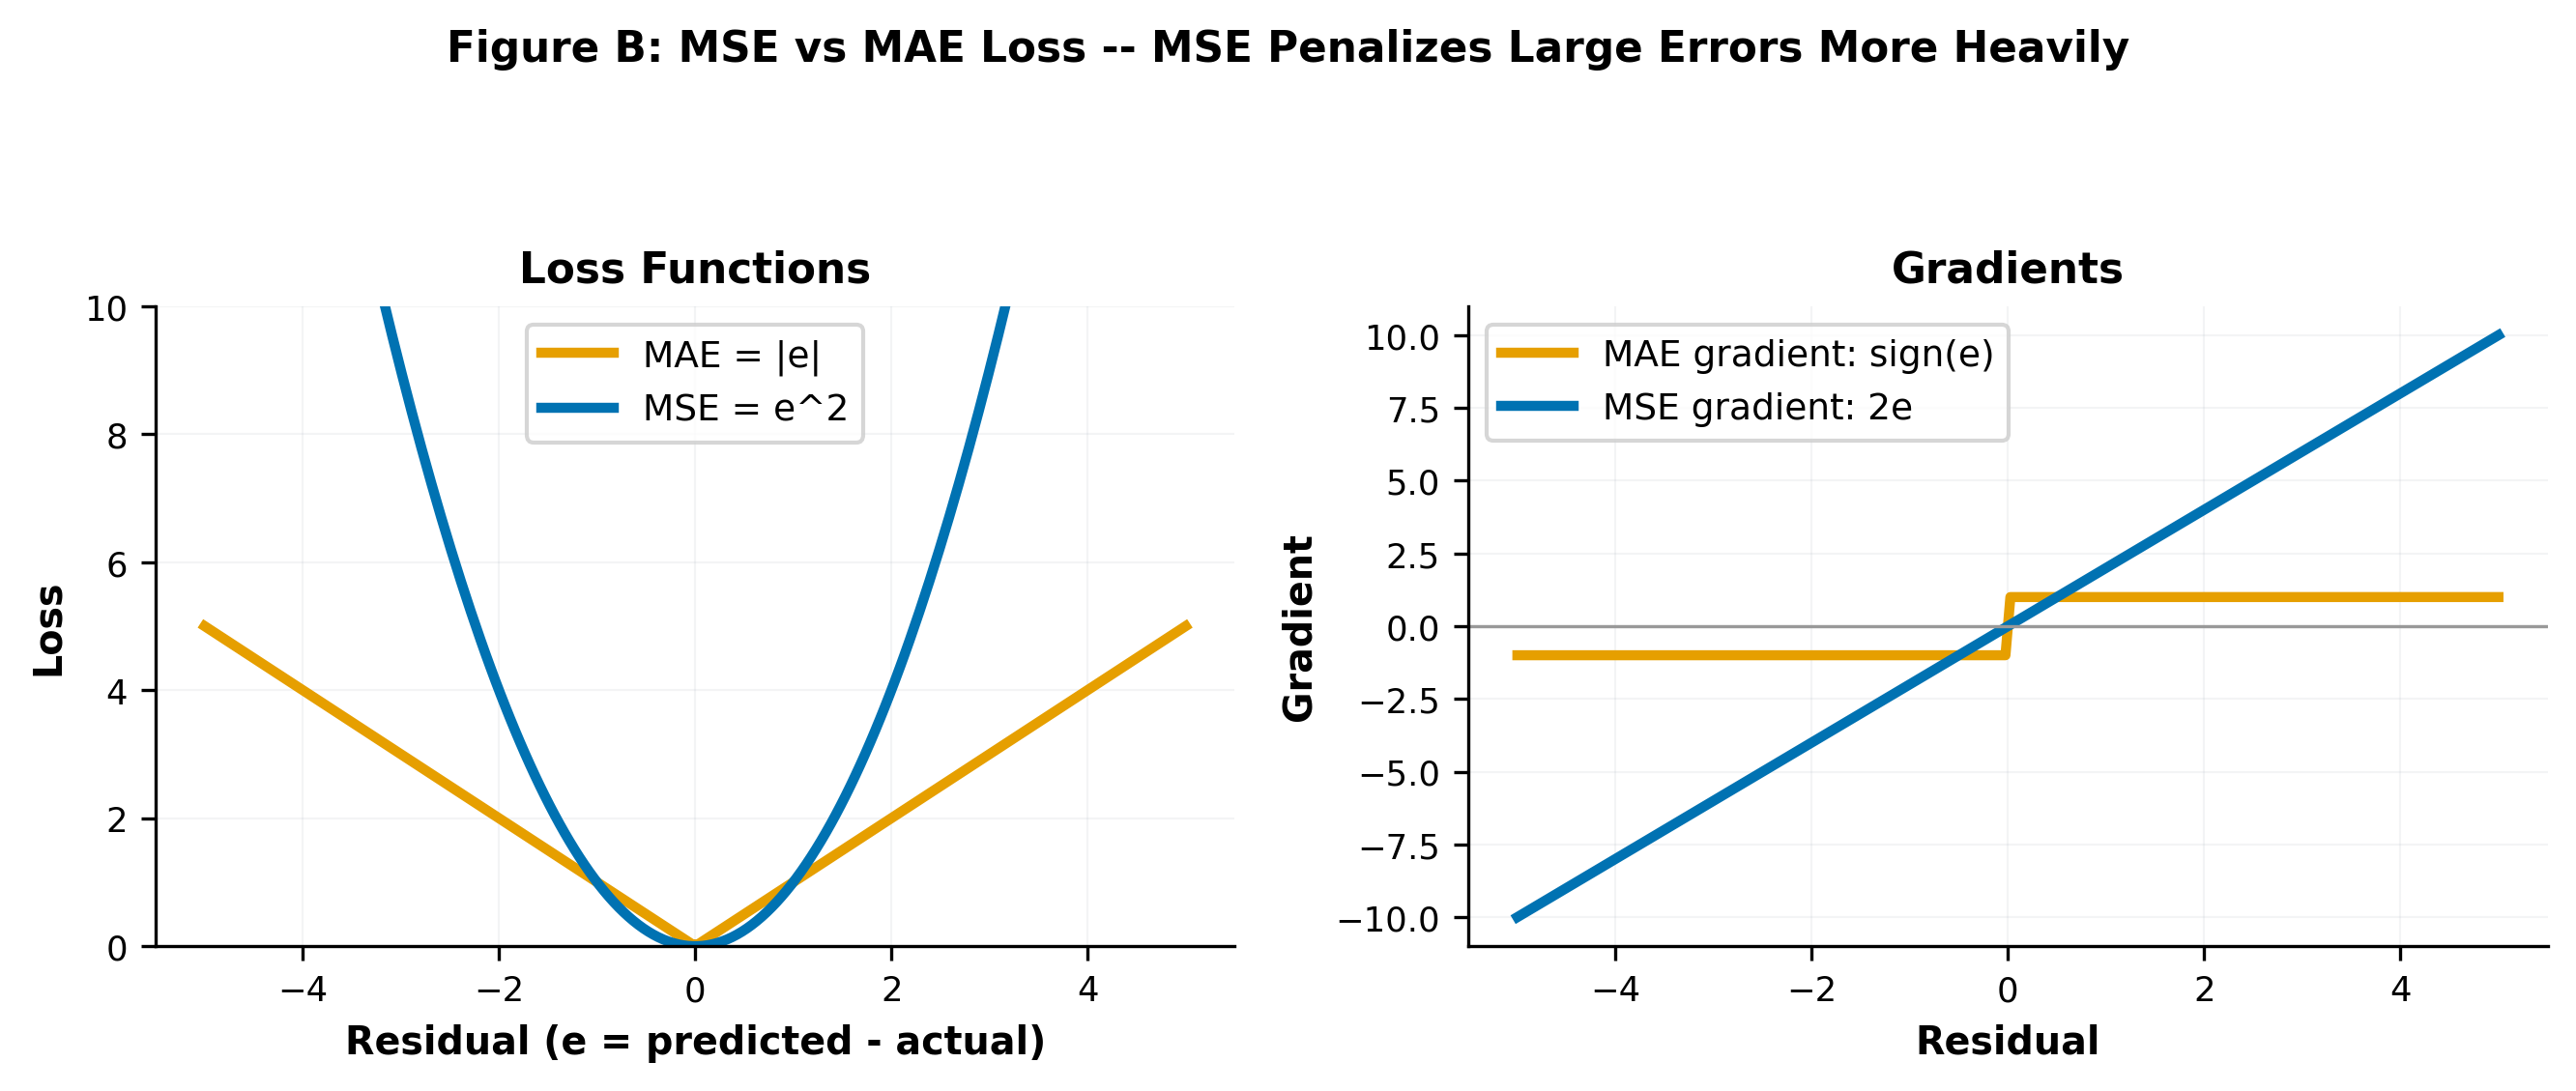
\includegraphics[width=0.9\linewidth]{11_figure_b.png}
\caption{MSE vs MAE loss functions and their gradients. MSE penalizes large errors more heavily, forcing the model to attend to extreme cases.}
\label{fig:mseMae}
\end{figure}

\subsection{Feature Selection}

With 2,520 candidate features and only $\sim$95 training subjects, feature selection is critical to prevent overfitting (Figure~\ref{fig:featselect}). We use XGBoost importance: an XGBoost model is trained to predict the target, and features are ranked by their total gain (improvement in the loss function when the feature is used for splitting). The top $K$ features are retained. $K=500$ was optimal for the CCC-optimized pipeline; $K=150$ sufficed for the MAE-optimized baseline. Selection is performed inside each cross-validation fold to prevent data leakage.

\begin{figure}[H]
\centering
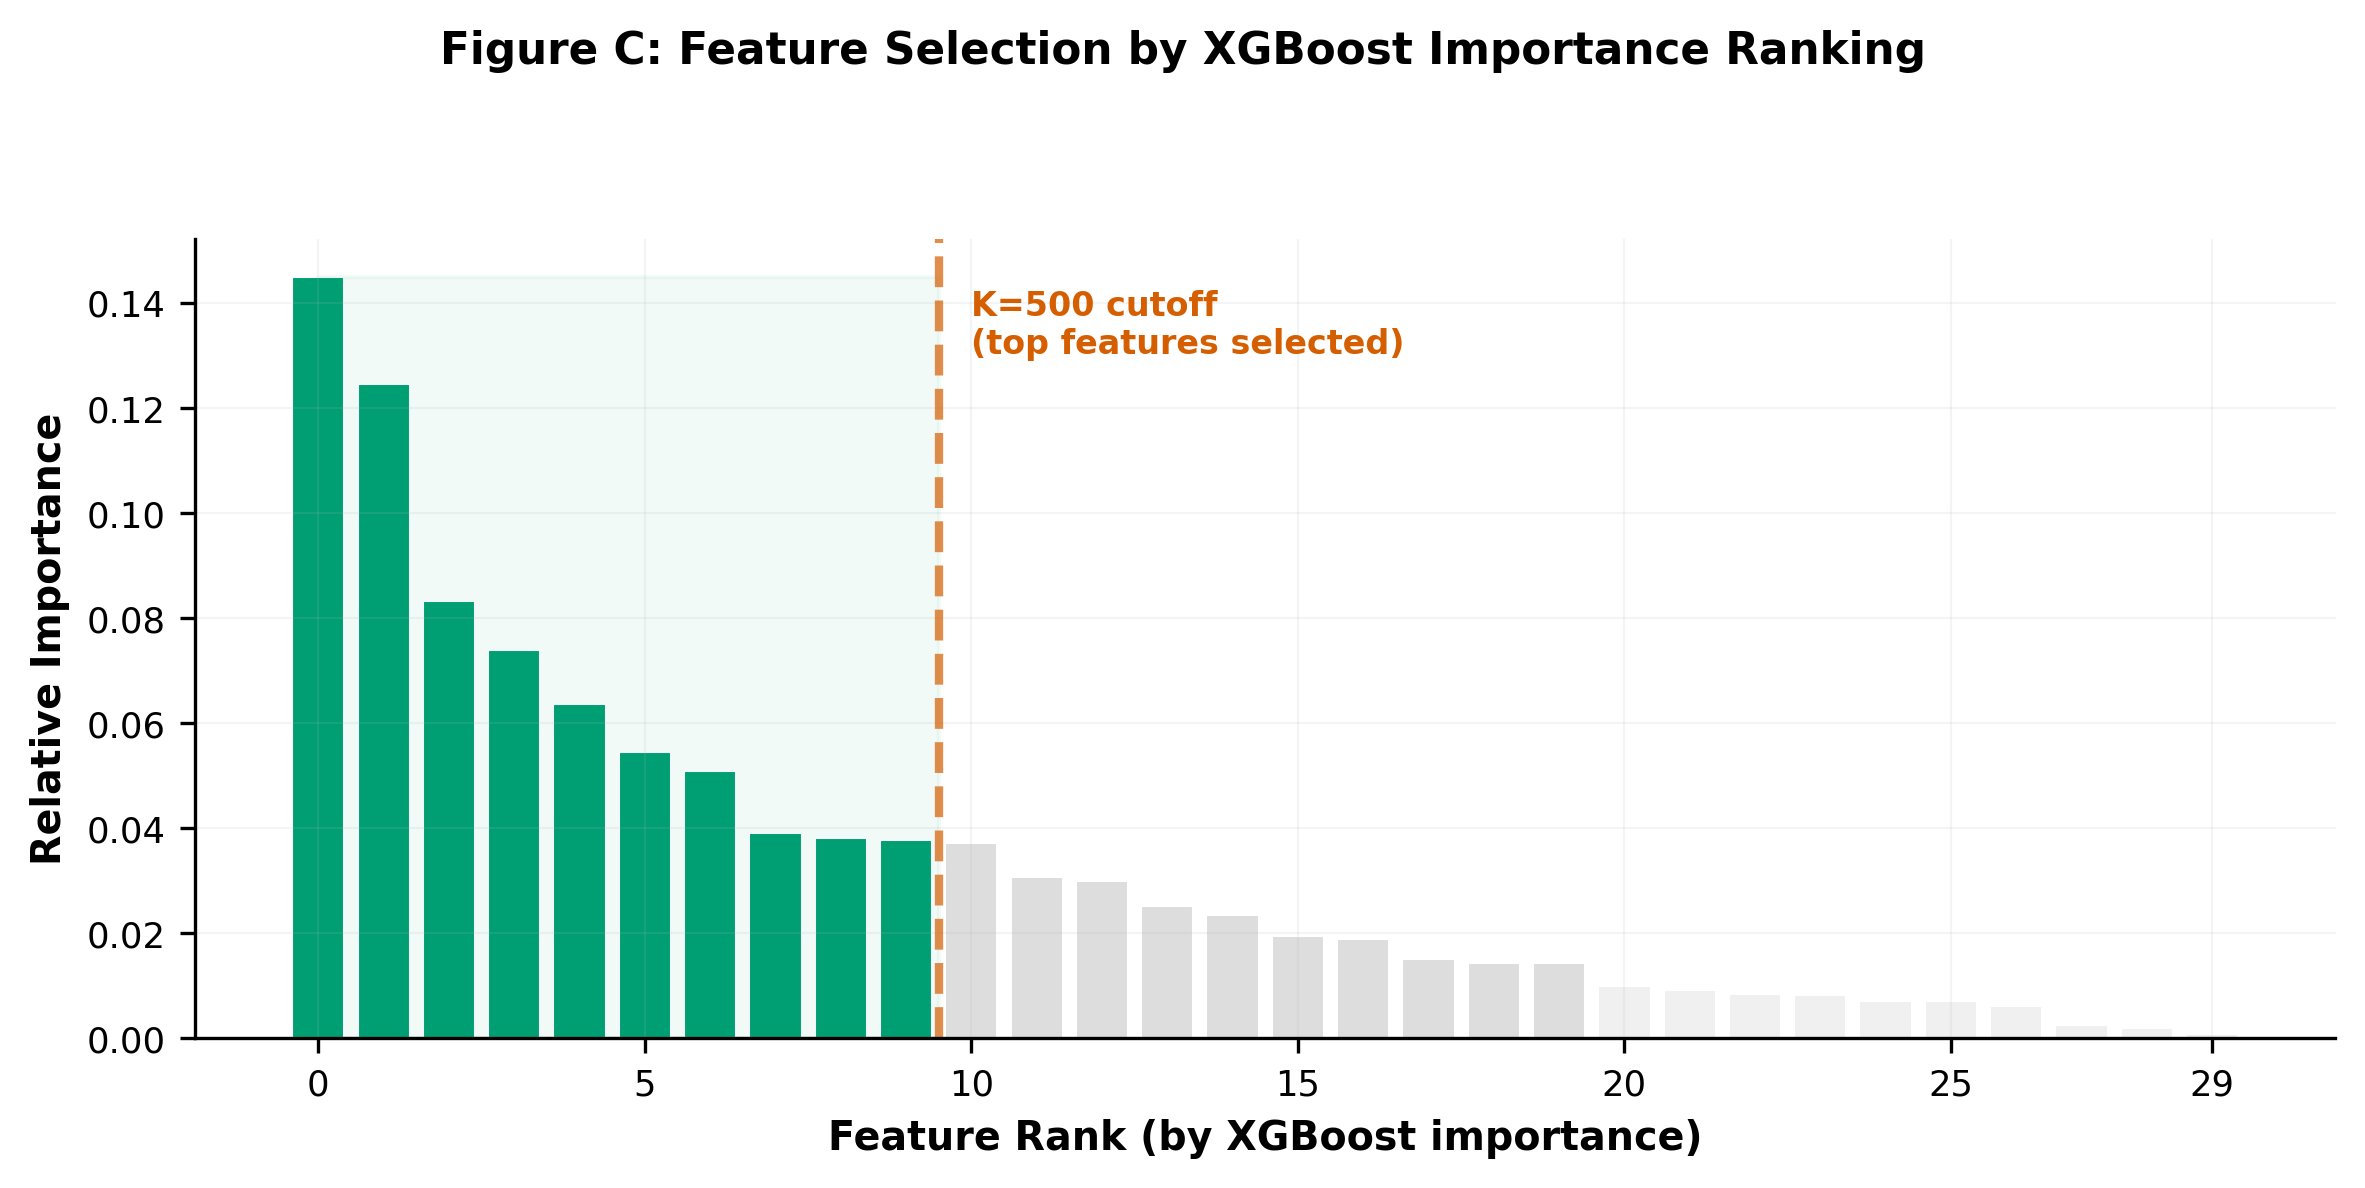
\includegraphics[width=0.9\linewidth]{12_figure_c.png}
\caption{Feature selection by XGBoost importance. Features ranked by total gain; top-$K$ retained (green). The cutoff balances signal retention against overfitting risk.}
\label{fig:featselect}
\end{figure}

\subsection{Multi-Seed Ensemble}

Individual model predictions vary with the random seed (which affects data shuffling, feature subsampling, and validation splits). Averaging predictions across 5 independent seeds (42, 123, 456, 789, 2024) reduces this variance (Figure~\ref{fig:seed}). The ensemble prediction is always at least as good as the average individual prediction, and typically better.

\begin{figure}[H]
\centering
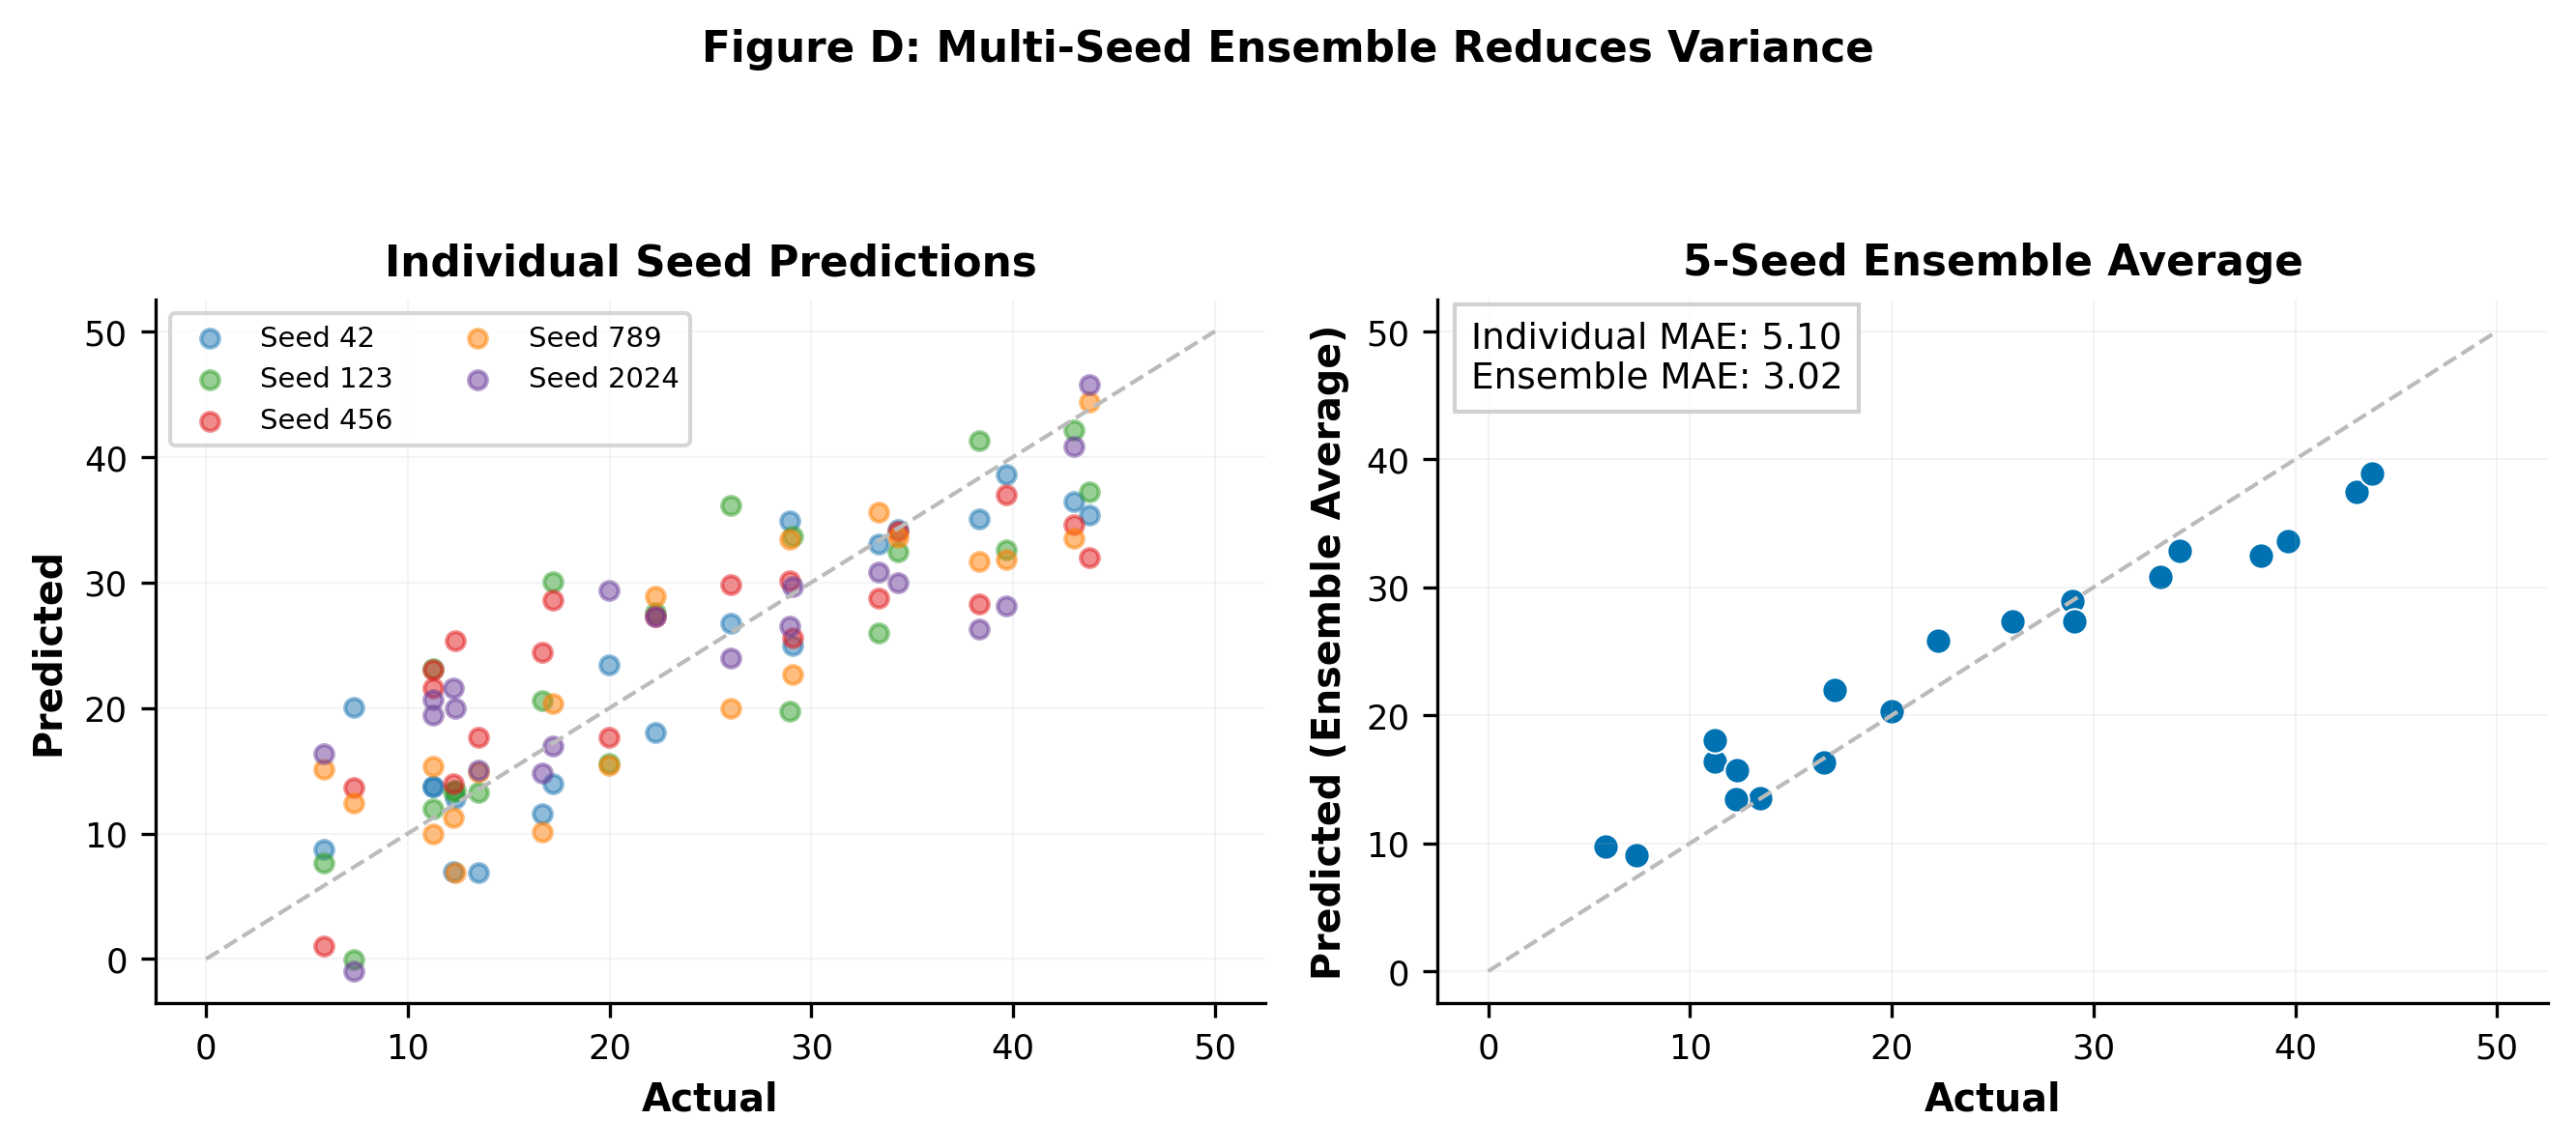
\includegraphics[width=0.9\linewidth]{13_figure_d.png}
\caption{Multi-seed ensemble averaging. Left: individual seed predictions show scatter. Right: 5-seed ensemble average is smoother and more accurate.}
\label{fig:seed}
\end{figure}

\subsection{Foundation Model Embedding Extraction}

MOMENT-1-base is a time-series foundation model pretrained on 385 public datasets\textsuperscript{10}. We use it as a frozen feature extractor (Figure~\ref{fig:fmemb}): raw IMU signals are truncated to 512 samples (5.12s), globally $z$-normalized, and passed through the frozen encoder. The resulting 768-dimensional embedding captures temporal patterns learned from diverse domains, supplementing handcrafted statistical features. No gradient computation or fine-tuning is performed, ensuring deterministic outputs.

\begin{figure}[H]
\centering
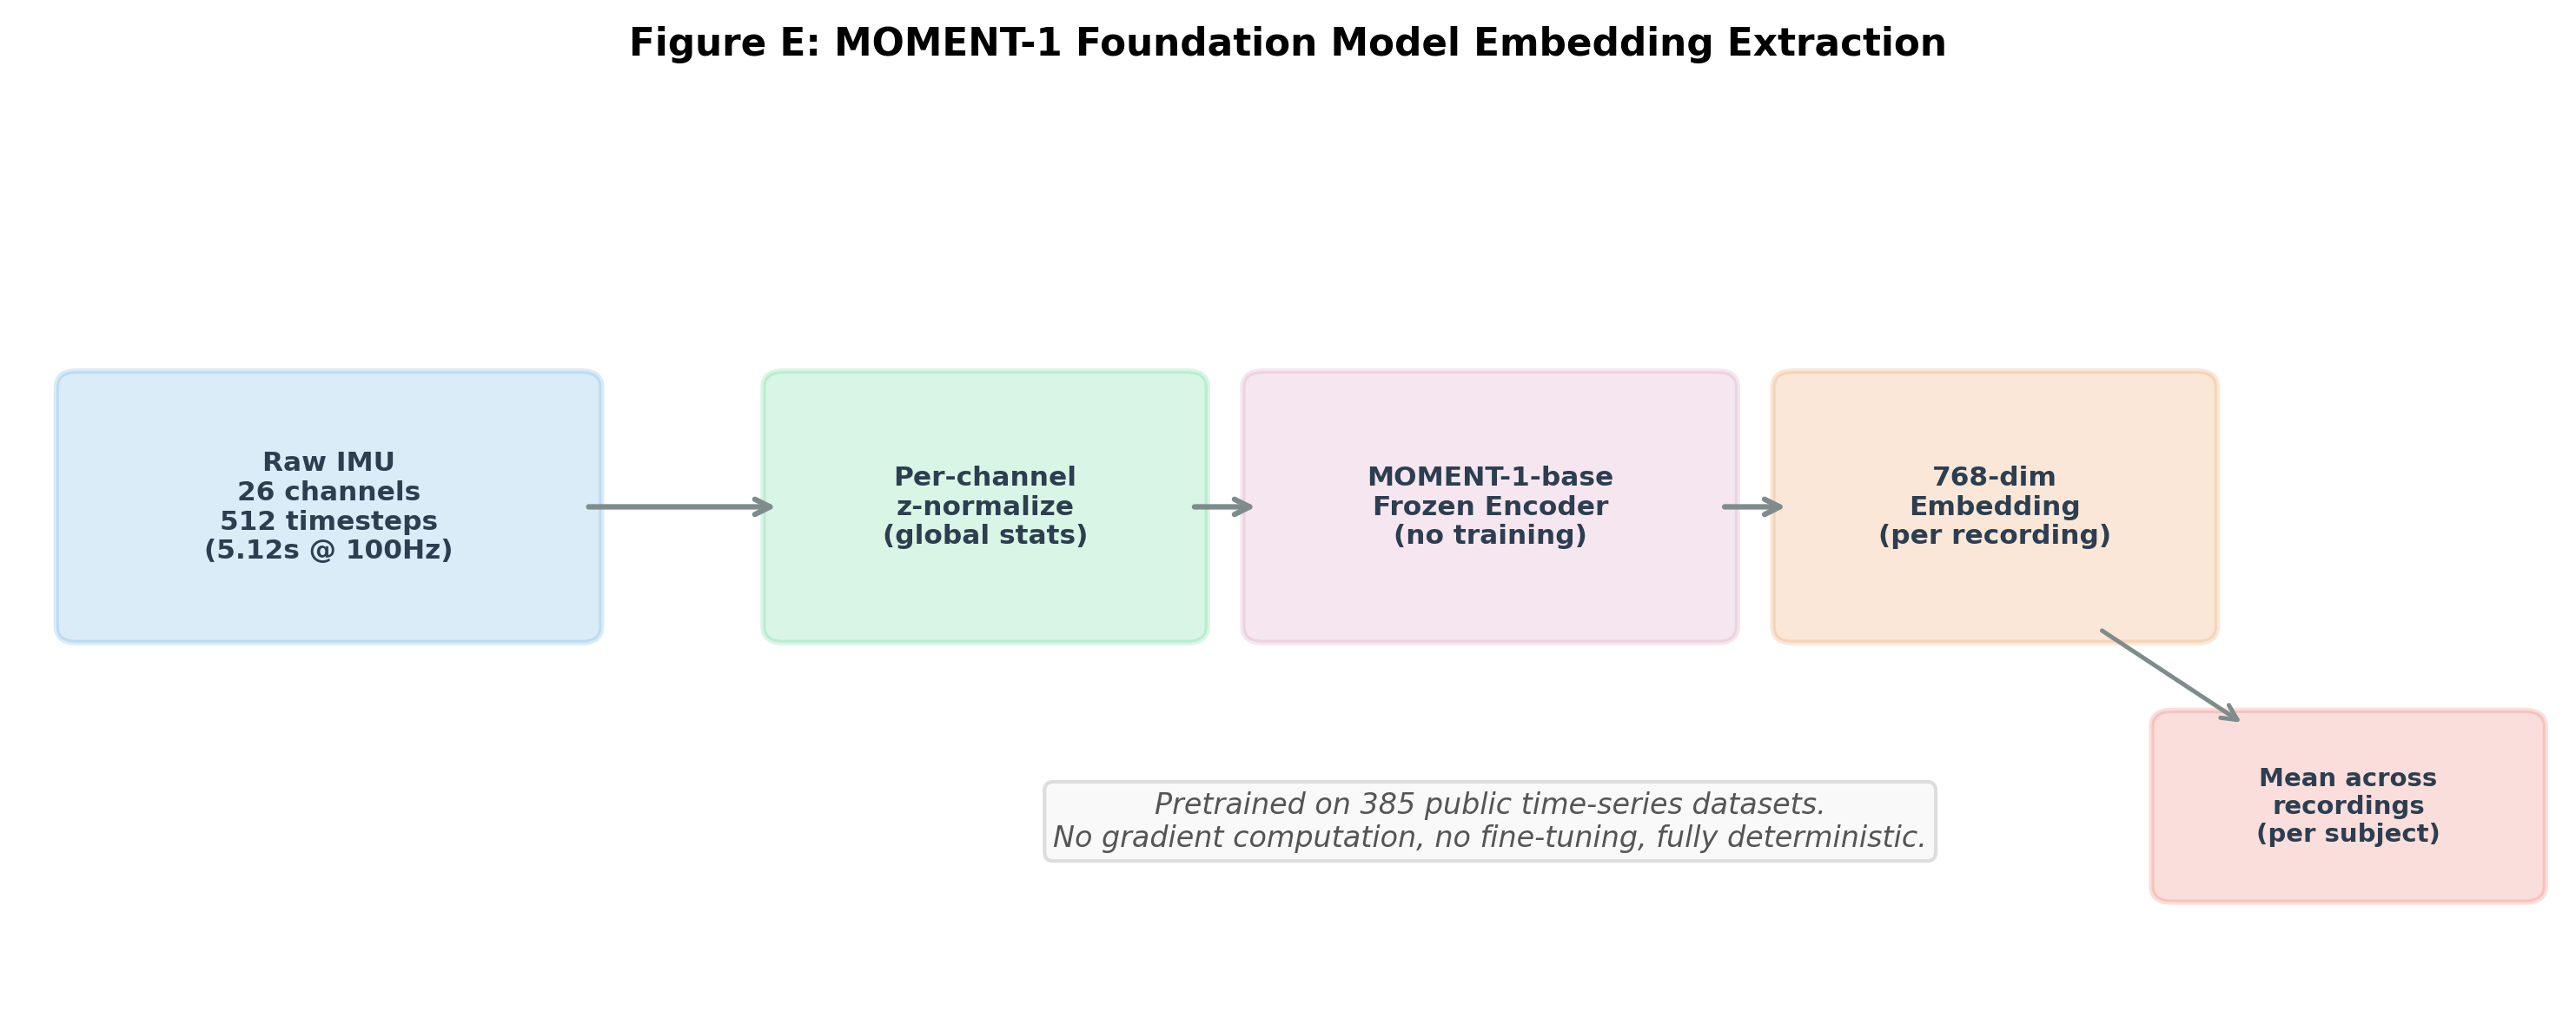
\includegraphics[width=0.9\linewidth]{14_figure_e.png}
\caption{MOMENT-1 foundation model embedding extraction. Raw IMU signals are normalized and passed through the frozen encoder to produce 768-dimensional embeddings, averaged across recordings per subject.}
\label{fig:fmemb}
\end{figure}

\subsection{Hyperparameter Choices}

Key hyperparameter differences between the baseline and CCC-optimized pipelines (Figure~\ref{fig:hp}): regularization (\texttt{reg\_lambda}: 3.0 to 0.3) was reduced to allow wider prediction range; \texttt{min\_data\_in\_leaf} (20 to 8) was the dominant knob for CCC improvement ($+0.105$); \texttt{colsample\_bytree} (1.0 to 0.5) introduced column subsampling for diversity; and objective (MAE to MSE) increased penalty on large errors. These changes collectively increased calibration slope from 0.40 to 0.69 on the observable subscore.

\begin{figure}[H]
\centering
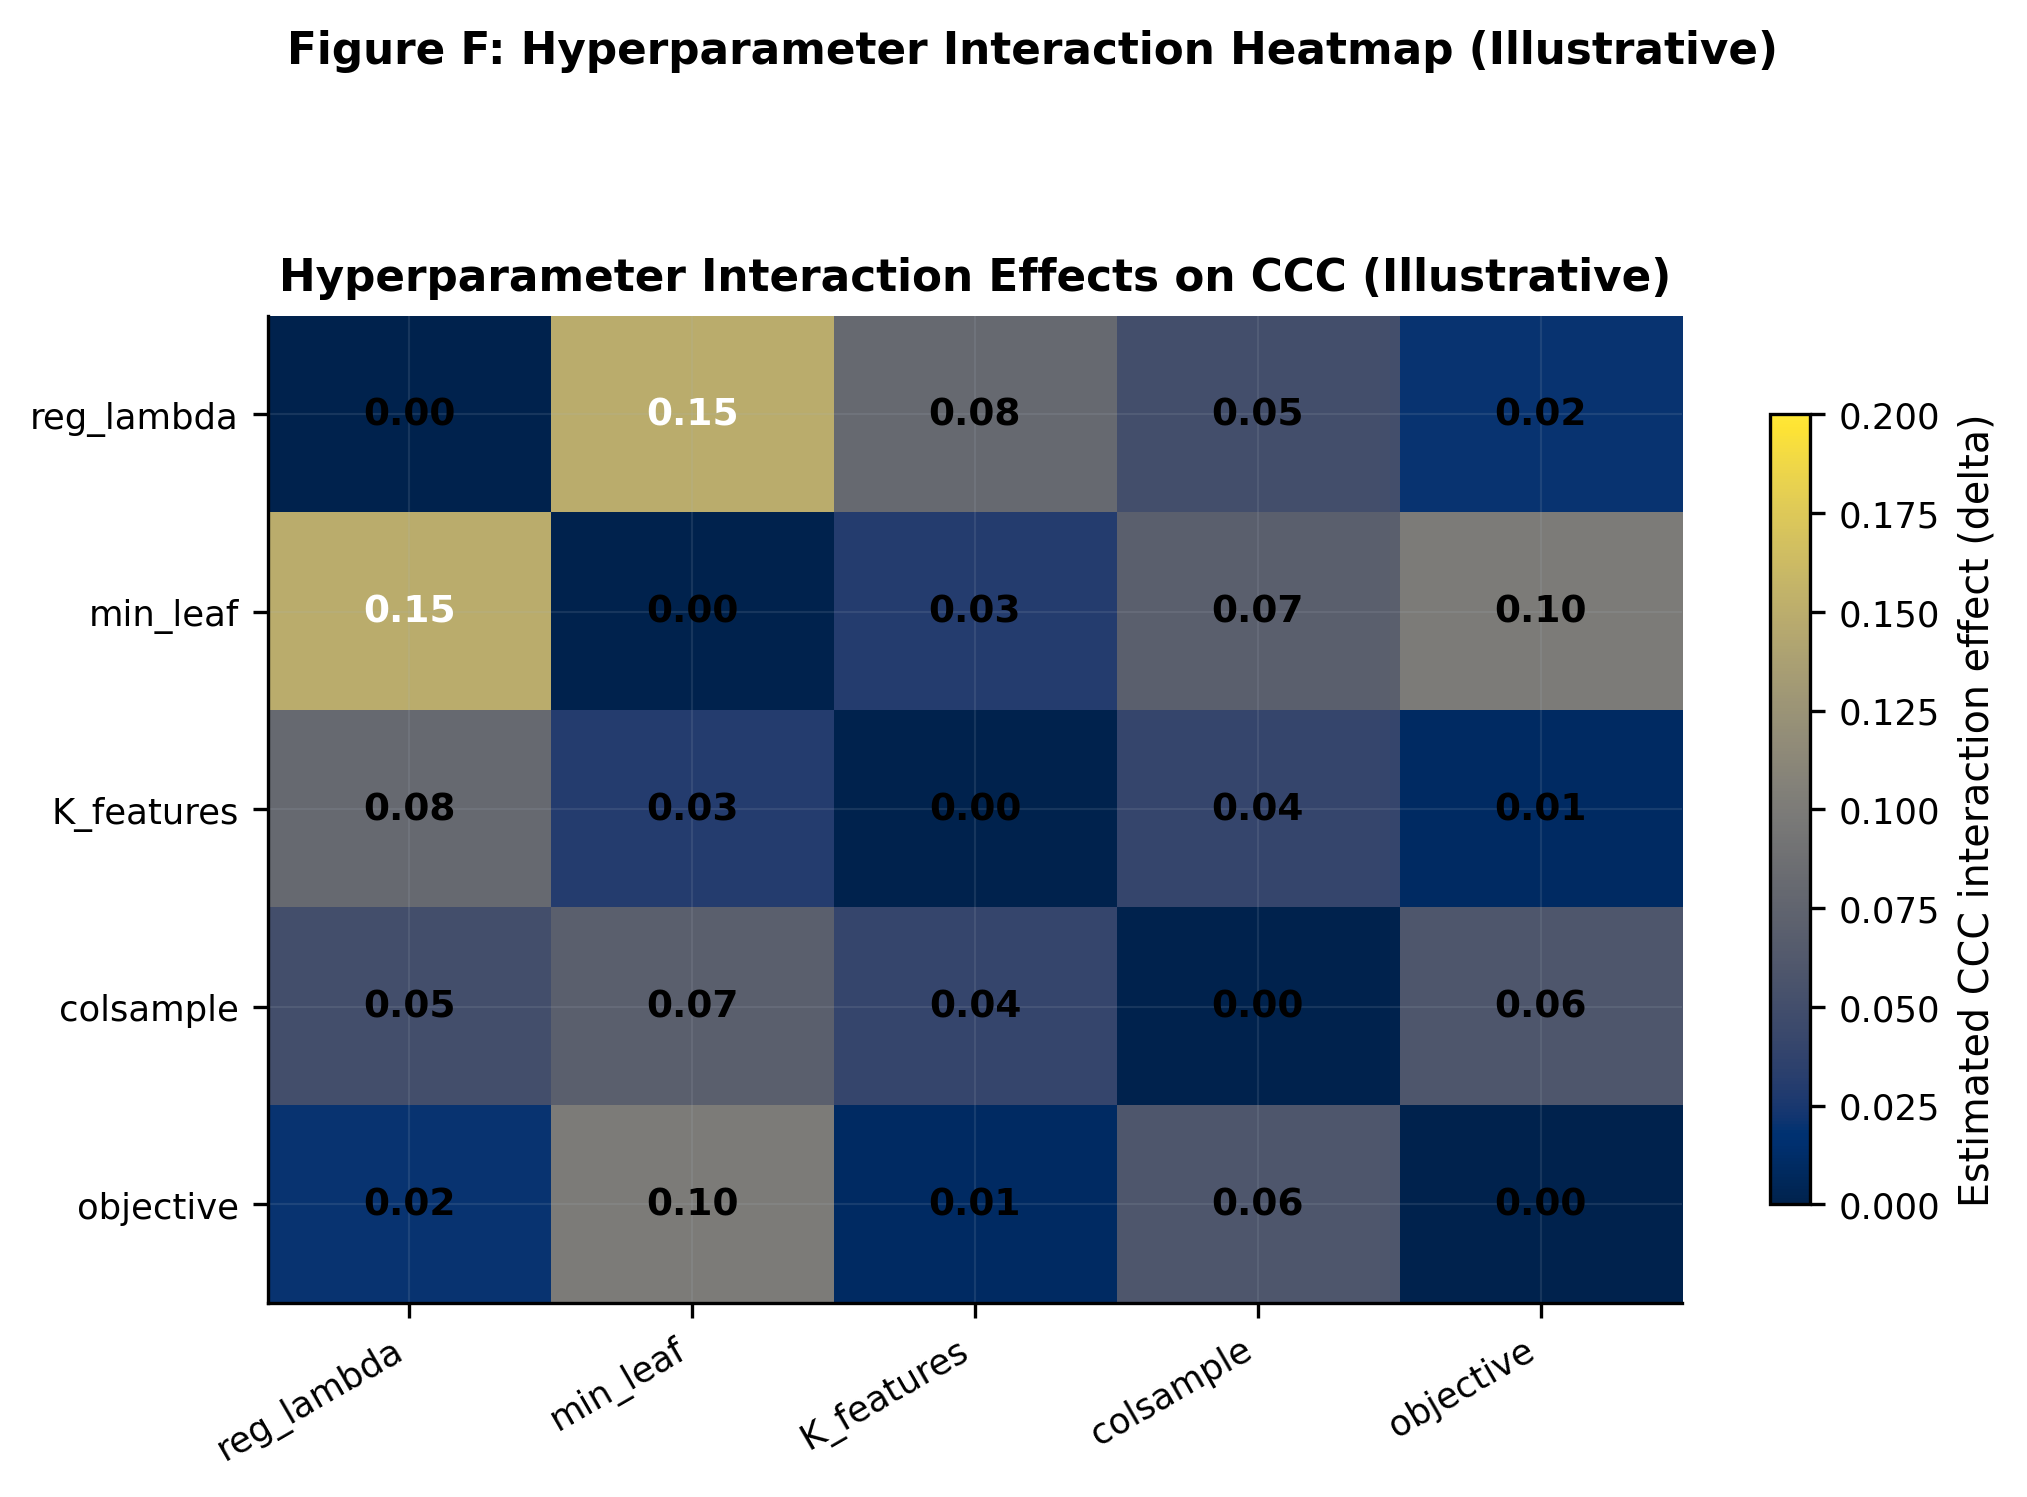
\includegraphics[width=0.9\linewidth]{15_figure_f.png}
\caption{Illustrative hyperparameter interaction effects on CCC (qualitative estimates, not directly measured). The strongest estimated interaction is between \texttt{reg\_lambda} and \texttt{min\_data\_in\_leaf}, reflecting the trade-off between regularization and leaf granularity.}
\label{fig:hp}
\end{figure}

% =========================================================
\section*{References}
% =========================================================
\begin{enumerate}[leftmargin=2.2em,itemsep=2pt]
\item GBD 2019 Collaborators. Global, regional, and national burden of neurological disorders, 1990--2019. \emph{Lancet Neurol.} 20, 797--820 (2021).
\item Horvath, K. et al. Minimal clinically important difference on the Motor Examination part of MDS-UPDRS. \emph{Parkinsonism Relat.\ Disord.} 21, 1421--1426 (2015).
\item Hssayeni, M.~D. et al. Wearable sensors for estimation of Parkinsonian tremor severity during free body movement. \emph{BioMed.\ Eng.\ OnLine} 20, 24 (2021).
\item Shuqair, H. et al. Self-supervised representation learning for motor severity estimation. \emph{Bioengineering} 11, 689 (2024).
\item Sotirakis, C. et al. Identification of motor progression in Parkinson's disease using wearable sensors. \emph{npj Parkinsons Dis.} 9, 74 (2023).
\item He, S. et al. Predicting levodopa response using wearable sensors. \emph{J.\ NeuroEng.\ Rehab.} 21, 47 (2024).
\item Li, J. et al. TRIP: Transformer-based IMU pretraining for Parkinson's disease. \emph{arXiv} 2510.15748 (2025).
\item Lin, L.~I.-K. A concordance correlation coefficient to evaluate reproducibility. \emph{Biometrics} 45, 255--268 (1989).
\item WearGait-PD dataset. \emph{Sci.\ Data} (2026). doi:10.1038/s41597-026-06806-2.
\item Goswami, M. et al. MOMENT: A family of open time-series foundation models. \emph{ICML} (2024).
\item Ke, G. et al. LightGBM: A highly efficient gradient boosting decision tree. \emph{NeurIPS} (2017).
\item Chen, T. \& Guestrin, C. XGBoost: A scalable tree boosting system. \emph{KDD} (2016).
\item Goetz, C.~G. et al. Movement Disorder Society-sponsored revision of the Unified Parkinson's Disease Rating Scale (MDS-UPDRS). \emph{Mov.\ Disord.} 23, 2129--2170 (2008).
\end{enumerate}

% =========================================================
\section*{Supplementary Information}
% =========================================================
\addcontentsline{toc}{section}{Supplementary Information}
% Supplementary tables and figures use manual "Table~SN." / "Figure~SN." labels
% because the HTML source's numbering is non-sequential (S2..S6 then S8, S7, S9, S10).
% We suppress automatic numbering and put the label inside caption text.
\captionsetup{labelformat=empty}

\subsection*{S1: Compression Ablation}

We evaluated five anti-compression proposals across three targets (Table~S2, Supplementary Figure~S1). Per-item ordinal classification (P1) degraded performance severely ($\mathrm{CCC}=0.338$). SMOGN tail augmentation (P3) and NGBoost distributional regression (P4) produced marginal improvements. Only ordinal ranking (P5) materially improved CCC on all targets. The mechanism involves two primary elements: (i)~ranking is a simpler task than regression (ordinal discrimination requires only preserved ordering), and (ii)~leaf features encode nonlinear severity partitions. HC ablation (Table~\ref{tab:hc}) confirms that the ranking transformation itself drives the improvement ($\Delta\mathrm{CCC}=0.001$ from HC inclusion); HC subjects provide optional, marginal calibration anchoring.

\begin{figure}[H]
\centering
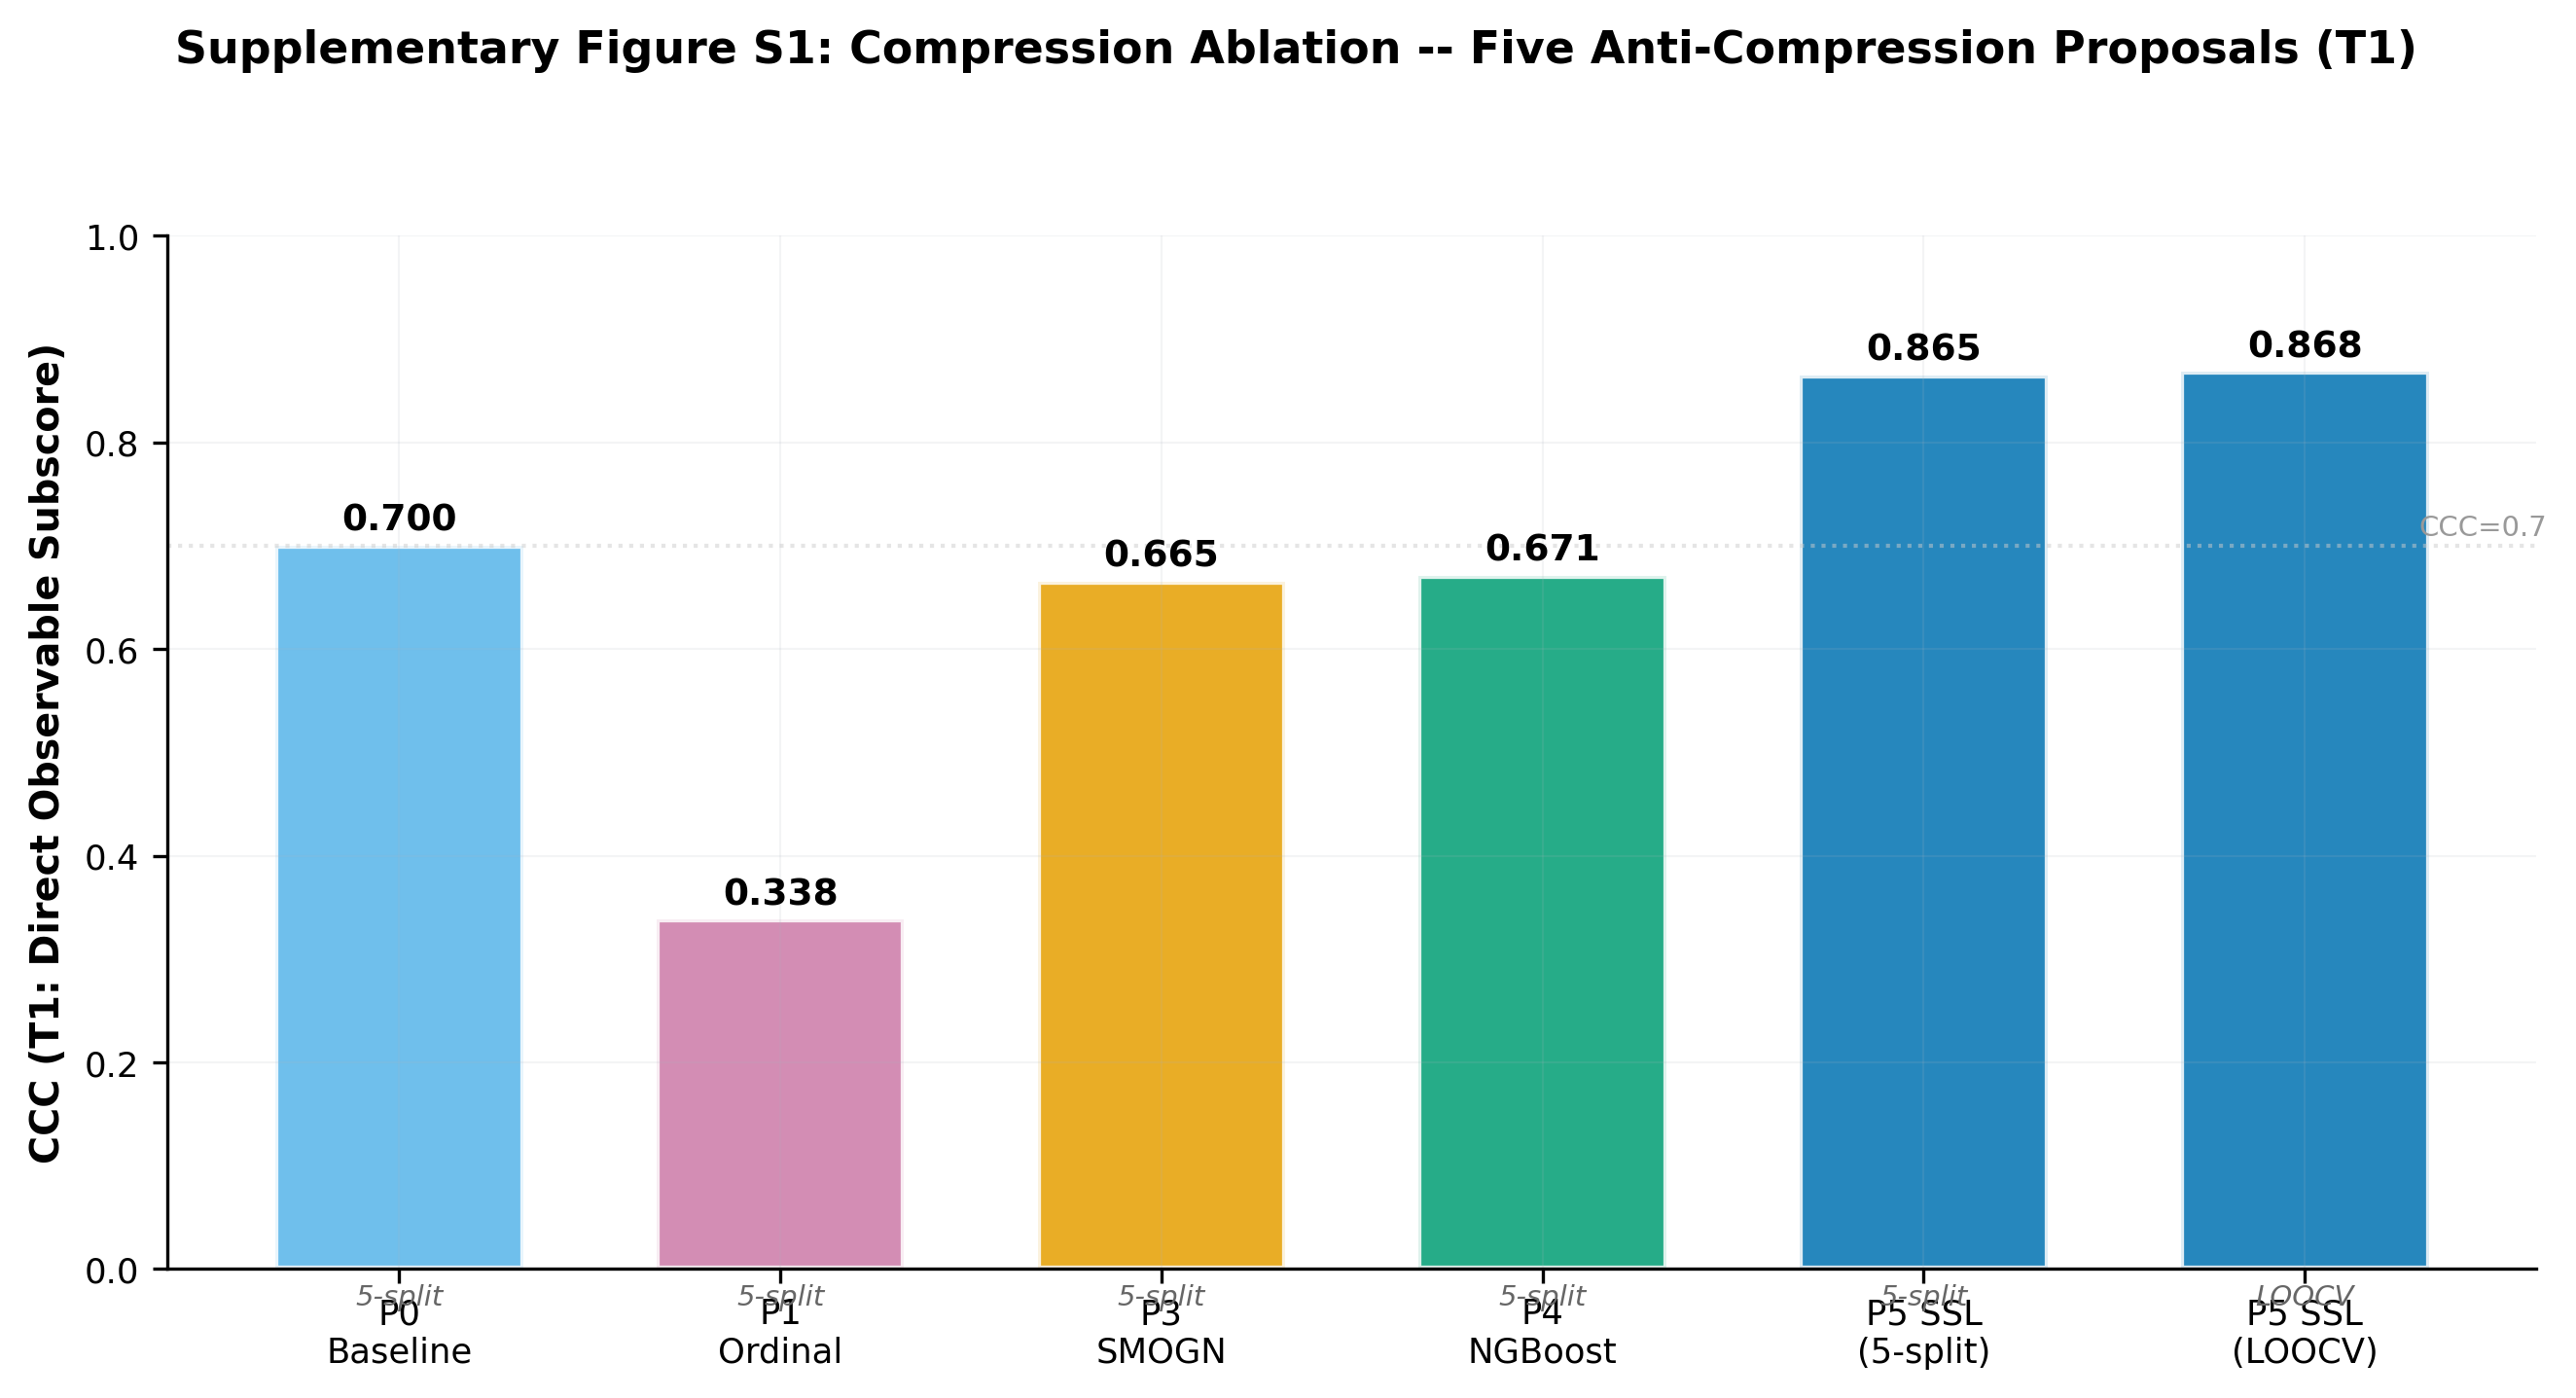
\includegraphics[width=0.9\linewidth]{16_supplementary_figure_s1.png}
\caption{\textbf{Figure~S1.} Compression ablation: five proposals evaluated on T1 (direct observable subscore, 5-fold CV). Only P5 ordinal ranking materially improves CCC. P1 ordinal classification degrades performance severely.}
\label{fig:s1compression}
\end{figure}

\begin{table}[H]
\centering
\caption{\textbf{Table~S2.} Compression ablation: five anti-compression proposals across three targets.}
\label{tab:compression}
\small
\resizebox{\textwidth}{!}{%
\begin{tabular}{llrrrrrrrr}
\toprule
& & & \multicolumn{3}{c}{\textbf{T1 (Direct Obs)}} & \multicolumn{2}{c}{\textbf{T2 (Broad Obs)}} & \multicolumn{2}{c}{\textbf{T3 (Total)}} \\
\cmidrule(lr){4-6}\cmidrule(lr){7-8}\cmidrule(lr){9-10}
\textbf{Proposal} & \textbf{Eval} & \textbf{$N$} & \textbf{CCC} & \textbf{Slope} & \textbf{MAE} & \textbf{CCC} & \textbf{MAE} & \textbf{CCC} & \textbf{MAE} \\
\midrule
P0 Baseline           & 5-split & 95 & 0.700 & 0.508 & 1.336 & 0.554 & 1.85 & 0.186 & 8.09 \\
P1 Ordinal Classif.   & 5-split & 95 & 0.338 & 0.184 & 1.594 & ---   & ---  & ---   & ---  \\
P3 SMOGN              & 5-split & 95 & 0.665 & 0.528 & 1.491 & 0.603 & 1.85 & 0.195 & 8.38 \\
P4 NGBoost            & 5-split & 95 & 0.671 & 0.484 & 1.387 & 0.595 & 1.75 & 0.187 & 8.20 \\
P5 Ordinal Ranking    & 5-split & 95 & \textbf{0.865} & 0.745 & 0.953 & \textbf{0.831} & 1.16 & \textbf{0.807} & 4.46 \\
P5 Ordinal Ranking    & LOOCV   & 94 & \textbf{0.868} & 0.689 & 0.986 & \textbf{0.852} & 1.33 & \textbf{0.776} & 4.65 \\
\bottomrule
\end{tabular}
}%
\tabnote{P0--P4: 5-split ($N=95$). P5 ordinal ranking shown under both 5-split ($N=95$, protocol-matched with P0--P4) and LOOCV ($N=94$, strictest evaluation). All rows show Stages~1--2 only (w/o temperature scaling) for protocol-matched comparison. P1 not run on T2/T3 (severely degraded on T1). P5 is the only proposal that materially improves CCC on any target.}
\end{table}

Ordinal ranking substantially reduces severity-dependent prediction bias (Table~S3, Supplementary Figure~S2). For T1 (5-split, apples-to-apples comparison): Q4 underprediction reduced from $-1.34$ to $-0.53$ (61\% reduction), Q2 overprediction nearly eliminated (from $+0.67$ to $+0.13$, 81\% reduction). The total UPDRS baseline (5-split) showed extreme compression: Q1 overpredicted by $+12$ points, Q4 underpredicted by $-12$ points. After ordinal ranking, T3 Q4 bias reduced from $-12.3$ to $-3.7$.

\begin{figure}[H]
\centering
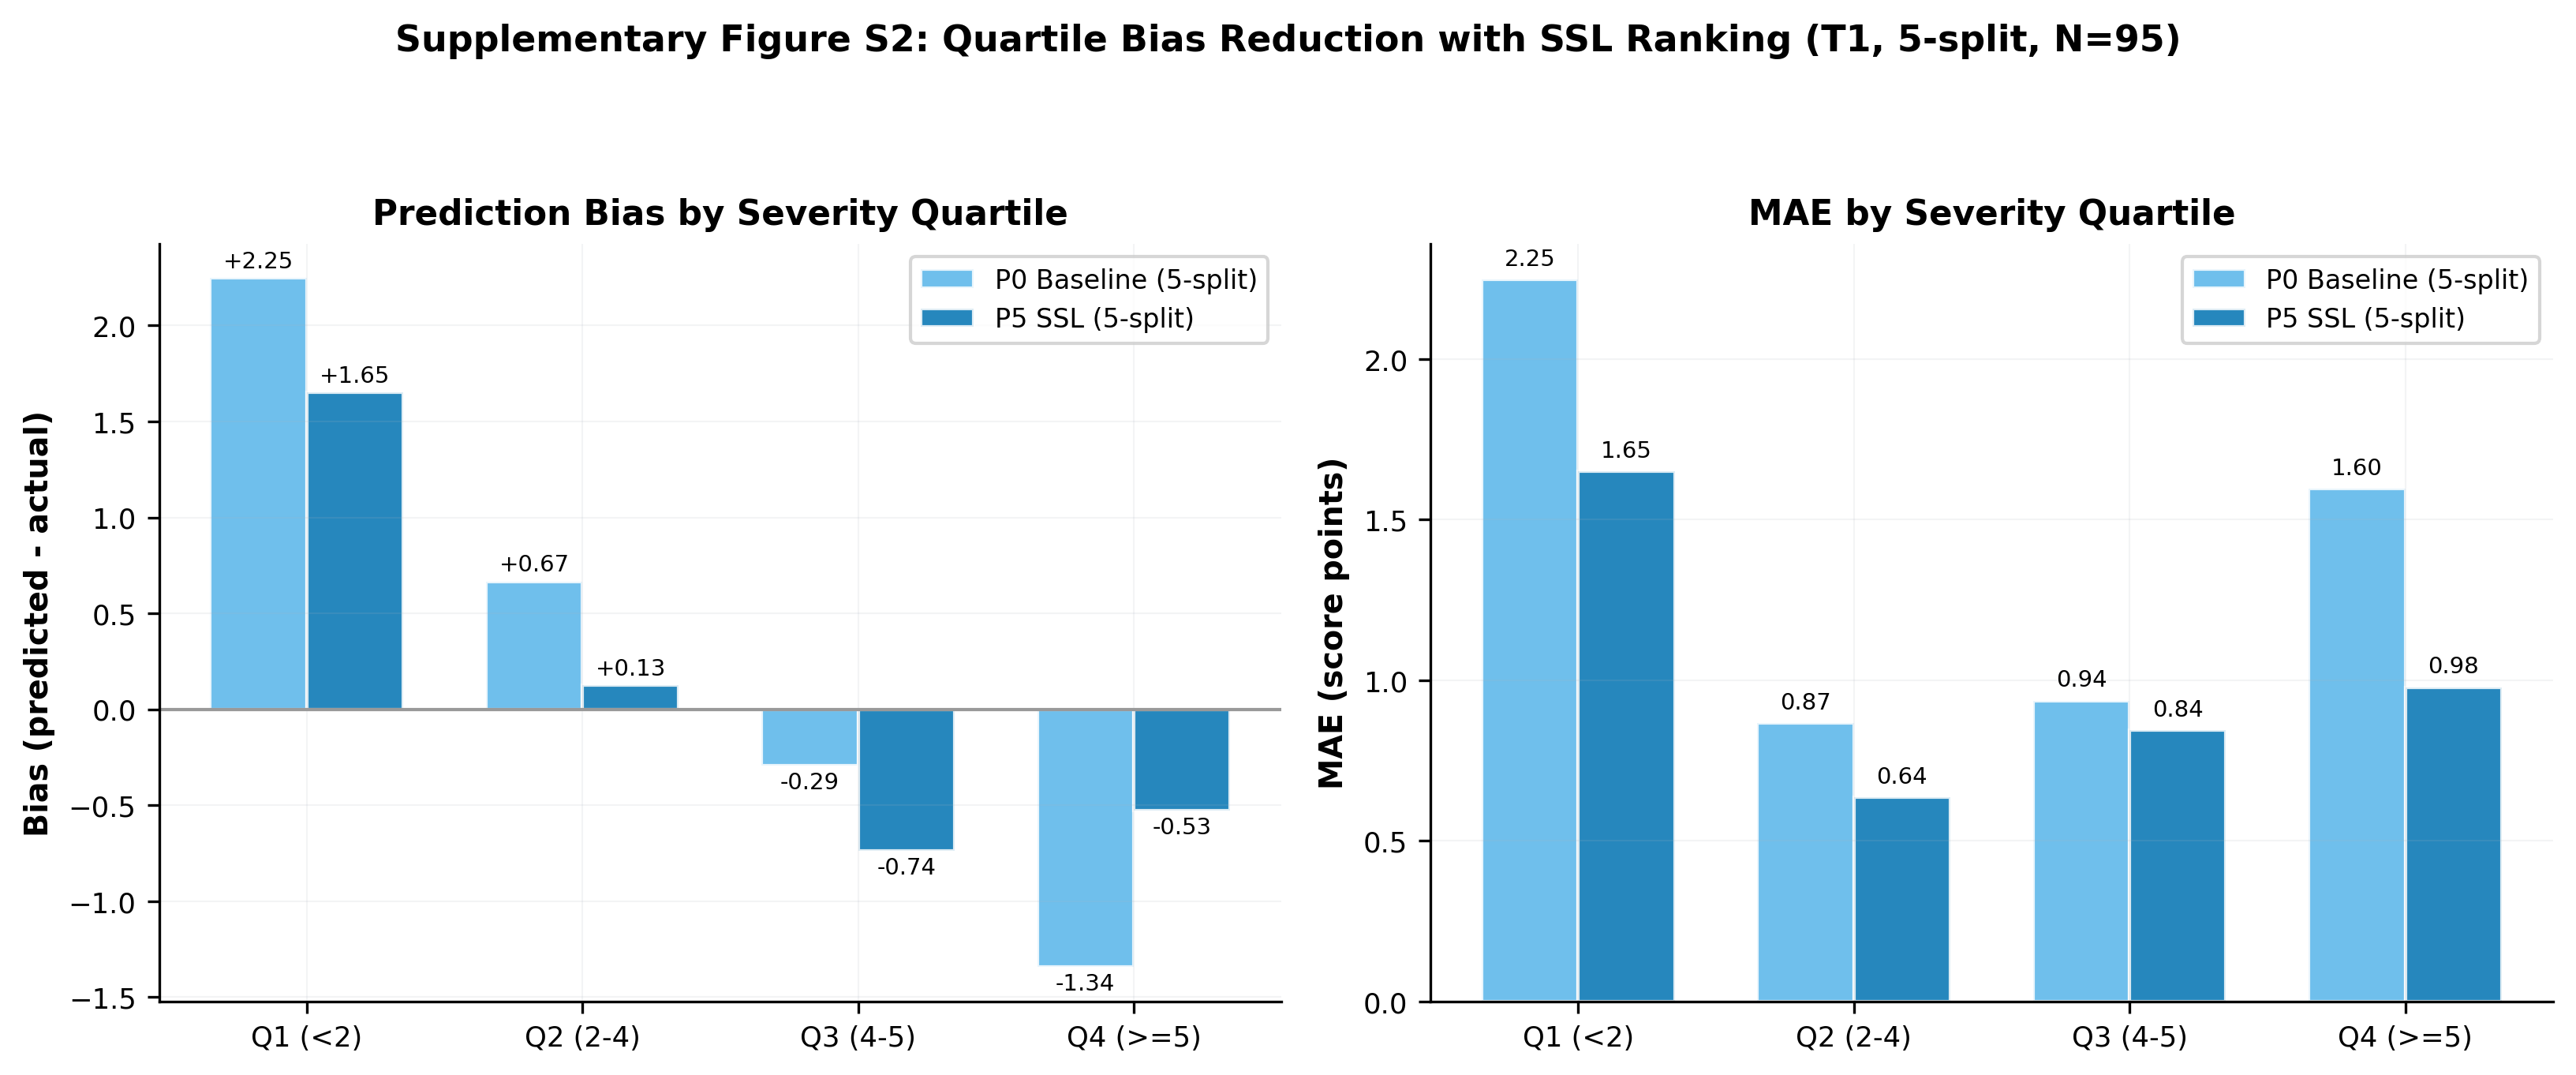
\includegraphics[width=0.9\linewidth]{17_supplementary_figure_s2.png}
\caption{\textbf{Figure~S2.} Quartile bias reduction with ordinal ranking (T1, 5-split comparison, $N=95$). Left: prediction bias by severity quartile. Right: MAE by quartile. Ordinal ranking (blue) reduces both bias and error across most quartiles compared to baseline (light blue). Values shown are pre-temperature (Stages~1--2 only).}
\label{fig:s2quartile}
\end{figure}

\begin{table}[H]
\centering
\caption{\textbf{Table~S3.} Quartile bias analysis: P0 baseline vs P5 ordinal ranking (both 5-split, $N=95$), T1 direct observable.}
\label{tab:quartile}
\small
\resizebox{\textwidth}{!}{%
\begin{tabular}{lrrrrrrr}
\toprule
& \multicolumn{3}{c}{\textbf{P0 Baseline (5-split)}} & \multicolumn{3}{c}{\textbf{P5 Ranking (5-split)}} & \\
\cmidrule(lr){2-4}\cmidrule(lr){5-7}
\textbf{Quartile} & \textbf{$N$} & \textbf{Bias} & \textbf{MAE} & \textbf{$N$} & \textbf{Bias} & \textbf{MAE} & \textbf{$|$Bias$|$ Change} \\
\midrule
Q1 ($<$2)   & 16 & $+2.25$ & 2.25 & 16 & $+1.65$ & 1.65 & $-27\%$ \\
Q2 (2--4)   & 31 & $+0.67$ & 0.87 & 31 & $+0.13$ & 0.64 & $-81\%$ \\
Q3 (4--5)   & 19 & $-0.29$ & 0.94 & 19 & $-0.74$ & 0.84 & $+151\%$ \\
Q4 ($\ge$5) & 29 & $-1.34$ & 1.60 & 29 & $-0.53$ & 0.98 & $-61\%$ \\
\bottomrule
\end{tabular}
}%
\tabnote{Both P0 and P5 use identical 5-split evaluation protocol ($N=95$) for apples-to-apples comparison. Bias $=$ mean(predicted $-$ actual).}
\end{table}

\subsection*{S2: Foundation Model Analysis}

Frozen MOMENT-1-base embeddings (768 dimensions, no fine-tuning) reduced mixed-cohort MAE from 8.49 to 7.77 (Wilcoxon $p=0.0039$; Supplementary Figure~S3). The advantage was non-significant in PD-only evaluation ($p_{\mathrm{adj}}=0.94$), suggesting FM embeddings primarily enhance PD-vs-HC discrimination rather than within-PD severity grading. FM embedding dimensions appeared among top features for the observable subscore (Figure~\ref{fig:featimp}), indicating complementary temporal pattern capture.

\begin{figure}[H]
\centering
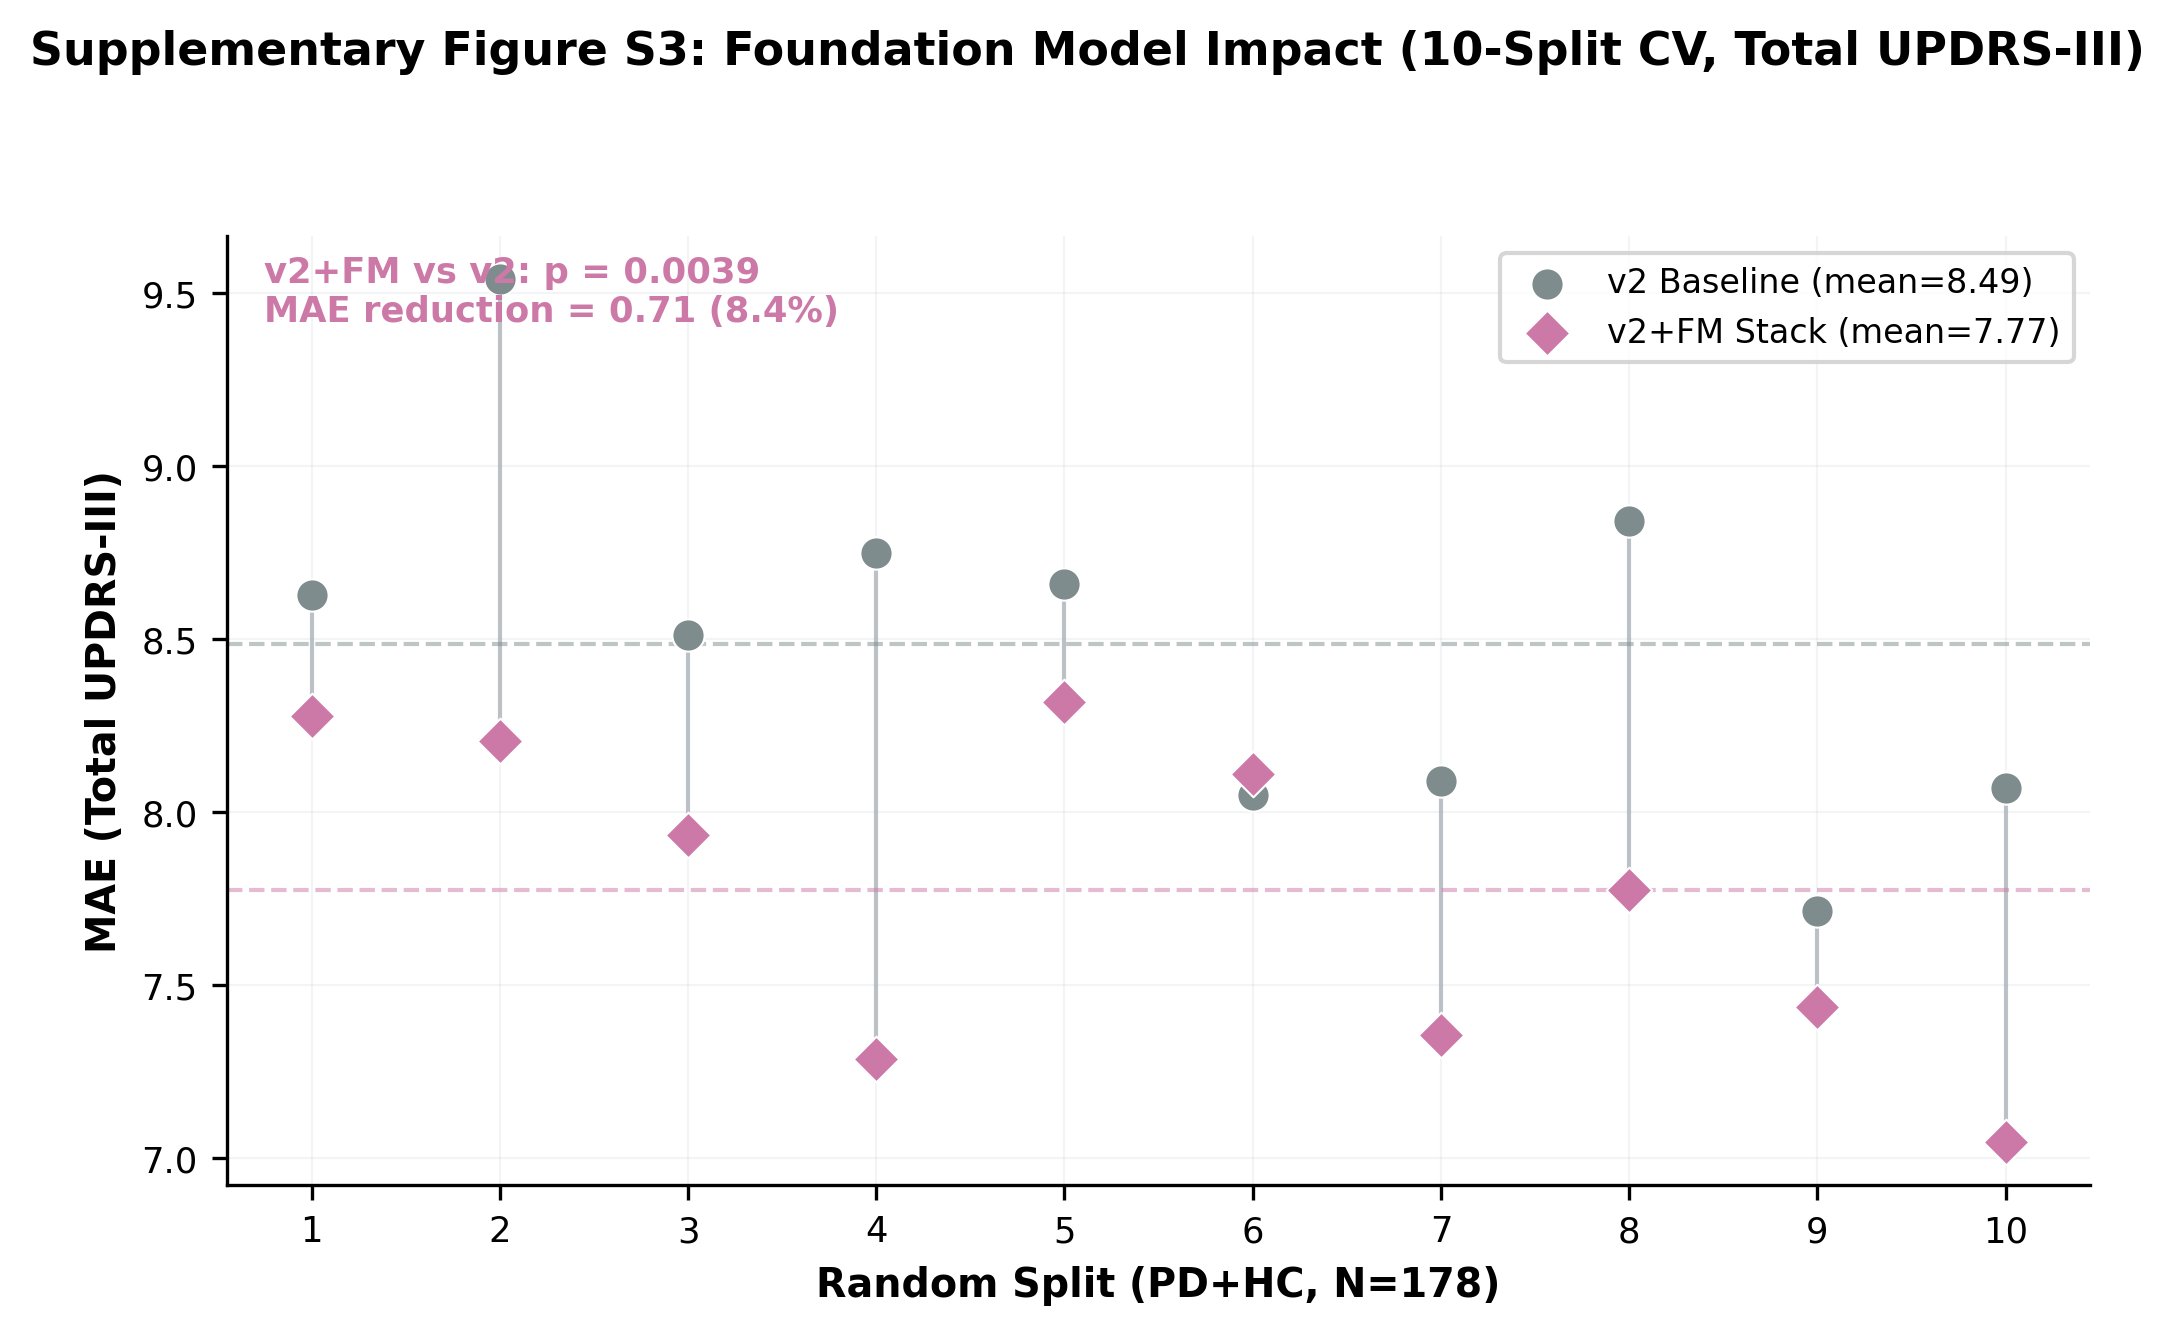
\includegraphics[width=0.9\linewidth]{18_supplementary_figure_s3.png}
\caption{\textbf{Figure~S3.} Foundation model impact across 10 splits (PD+HC, $N=178$, total UPDRS-III). v2+FM stack (purple diamonds) consistently outperforms v2 baseline (grey circles). Paired Wilcoxon $p=0.0039$.}
\label{fig:s3fm}
\end{figure}

\subsection*{S3: Sensor Ablation}

FM re-extraction per sensor configuration eliminates data leakage (Table~S4). The 5-sensor minimal set (lower back, bilateral wrists, bilateral ankles) matches the full 13-sensor configuration (7.67 vs 7.72, $p=0.85$). Even 2 wrist sensors achieved competitive performance ($p=0.55$). These results are for total UPDRS-III (10-split CV). For the observable subscore (T1) under ordinal ranking (5-fold CV), single-sensor analysis (Table~S5) reveals that a single lower back sensor achieves $\mathrm{CCC}=0.867$, matching the full 13-sensor configuration ($\mathrm{CCC}=0.857$). Single wrist sensors achieve $\mathrm{CCC}>0.78$, supporting smartwatch-based clinical deployment.

\begin{table}[H]
\centering
\caption{\textbf{Table~S4.} Sensor ablation (PD-only 10-split, total UPDRS-III, FM re-extracted per config).}
\label{tab:sensor10split}
\begin{tabular}{lrrrr}
\toprule
\textbf{Configuration} & \textbf{$N$ Sensors} & \textbf{MAE $\pm$ SD} & \textbf{CCC} & \textbf{$p$ vs All 13} \\
\midrule
All 13 sensors                  & 13 & $7.72 \pm 0.78$ & 0.184 & ---   \\
Minimal 5 (back+wrists+ankles)  &  5 & $7.67 \pm 0.84$ & 0.152 & 0.851 \\
Back + wrists (3)               &  3 & $7.89 \pm 0.64$ & 0.113 & 0.202 \\
Wrists only (2)                 &  2 & $7.80 \pm 0.63$ & 0.102 & 0.555 \\
Lower back only (1)             &  1 & $8.12 \pm 0.76$ & 0.048 & 0.014 \\
\bottomrule
\end{tabular}
\tabnote{FM embeddings re-extracted per sensor configuration to prevent data leakage. Results are for total UPDRS-III, not observable subscore.}
\end{table}

\begin{table}[H]
\centering
\caption{\textbf{Table~S5.} Single-sensor ordinal ranking performance (T1 observable subscore, 5-fold CV).}
\label{tab:singlesensor}
\resizebox{\textwidth}{!}{%
\begin{tabular}{lrrrrrr}
\toprule
\textbf{Sensor Configuration} & $N_{\mathrm{sensors}}$ & $N_{\mathrm{features}}$ & \textbf{CCC} & \textbf{MAE} & \textbf{slope} & \textbf{$r$} \\
\midrule
LowerBack (1) &  1 &  318 & 0.867 & 0.962 & 0.726 & 0.884 \\
R\_Wrist (1)  &  1 &  155 & 0.784 & 1.202 & 0.644 & 0.806 \\
L\_Wrist (1)  &  1 &  137 & 0.791 & 1.187 & 0.662 & 0.806 \\
wrists (2)    &  2 &  261 & 0.776 & 1.206 & 0.606 & 0.809 \\
all (13)      & 13 & 1721 & 0.857 & 1.001 & 0.720 & 0.873 \\
\bottomrule
\end{tabular}
}%
\tabnote{A single lower back sensor achieves $\mathrm{CCC}=0.867$, matching the full 13-sensor configuration ($\mathrm{CCC}=0.857$). Single wrist achieves $\mathrm{CCC}>0.78$, supporting smartwatch-based clinical deployment.}
\end{table}

\subsection*{S4: Negative Results}

Negative results strengthen the ceiling argument. Seven deep learning configurations (Transformer, InceptionTime, SensorGNN; Table~S6) all produced $\mathrm{MAE}>10$, consistent with overfitting at $N=178$. Additional failed approaches included: item decomposition (52\% worse), mixture-of-experts, cross-sensor coordination features, and freezing-of-gait transfer ($\mathrm{AUC}=0.500$). Among the five anti-compression proposals, only ordinal ranking produced material CCC improvement; per-item ordinal classification, pairwise contrastive boosting, SMOGN augmentation, and NGBoost distributional regression all failed (Table~S2). This convergence of diverse approaches on a compression ceiling supports the interpretation that the barrier is representational rather than purely methodological.

\begin{table}[H]
\centering
\caption{\textbf{Table~S6.} Deep learning architectures (all MAE $>10$ on held-out test, seed$=42$ split).}
\label{tab:dl}
\resizebox{\textwidth}{!}{%
\begin{tabular}{lrrr}
\toprule
\textbf{Architecture} & \textbf{Mean MAE $\pm$ SD} & \textbf{Ensemble MAE} & \textbf{Ensemble $r$} \\
\midrule
P1A: MAE$\rightarrow$Transformer 128d/4L + MIL        & $11.88 \pm 2.70$ & 10.85 & 0.590 \\
P1B: Contrastive$\rightarrow$Transformer 128d/4L + MIL& $12.96 \pm 2.22$ & 11.70 & 0.349 \\
P1C: Transformer 128d/4L + MIL (scratch)              & $11.96 \pm 2.54$ & 10.99 & 0.521 \\
P3A: InceptionTime 3blk + MIL                         & $13.22 \pm 1.87$ & 11.87 & 0.470 \\
P3B: InceptionTime 3blk + ordinal                     & $11.93 \pm 0.93$ & 10.46 & 0.436 \\
P3C: InceptionTime 3blk h24 + MIL                     & $12.84 \pm 0.94$ & 12.01 & 0.443 \\
P6A: SensorGNN 64d + MIL                              & $13.80 \pm 0.61$ & 13.68 & 0.454 \\
\bottomrule
\end{tabular}%
}

\tabnote{All DL models trained end-to-end on raw IMU windows (10s, 50\% overlap). $N=178$ insufficient for end-to-end deep learning. Held-out test $N=36$.}
\end{table}

\subsection*{S5: Calibration Ablation}

Seven calibration methods were evaluated on the T1 observable subscore (LOOCV, $N=94$). Results are presented in Table~S8.

\begin{table}[H]
\centering
\caption{\textbf{Table~S8.} Calibration ablation: seven methods for correcting prediction compression (T1 observable, LOOCV, $N=94$).}
\label{tab:calib}
\small
\resizebox{\textwidth}{!}{%
\begin{tabular}{lrrrrl}
\toprule
\textbf{Experiment} & \textbf{CCC} & \textbf{Cal.\ slope} & \textbf{MAE} & \textbf{std ratio} & \textbf{Verdict} \\
\midrule
E0: Baseline (5-seed LGB ensemble)       & 0.859 & 0.691 & 1.046 & 0.779 & Reference \\
E1: CCC custom loss objective            & 0.345 & 0.322 & 2.461 & 0.516 & Failed --- gradient too noisy at $N=94$ \\
E2: Quantile regression (median)         & 0.800 & 0.562 & 1.109 & 0.633 & Failed --- worse than baseline \\
E3: Distance-weighted KNN ($K=3$)        & 0.872 & 0.951 & 1.228 & 1.080 & Good calibration \\
E4: Variance penalty ($\lambda=0.1$)     & 0.846 & 0.671 & 1.078 & 0.763 & Marginal --- slope barely moved \\
E5: Conformal quantile regression        & 0.863 & 0.952 & 1.207 & 1.098 & Good calibration \\
E6: Ridge on PCA leaf features           & 0.467 & 0.523 & 1.947 & 1.105 & Failed --- linear head too weak \\
\textbf{E7: Temperature scaling ($T=1.4$)} & \textbf{0.882} & \textbf{0.967} & \textbf{1.162} & \textbf{1.090} & \textbf{Best --- simplest, best CCC+slope} \\
\bottomrule
\end{tabular}%
}

\tabnote{Source: \texttt{run\_calibration\_v2.py}. E7 temperature scaling achieves the best combination of CCC and calibration slope with a single parameter. std ratio $=$ std(predictions)/std(true values); target $\ge 0.92$. E3 (KNN) and E5 (CQR) also achieve good calibration but are more complex.}
\end{table}

\begin{figure}[H]
\centering
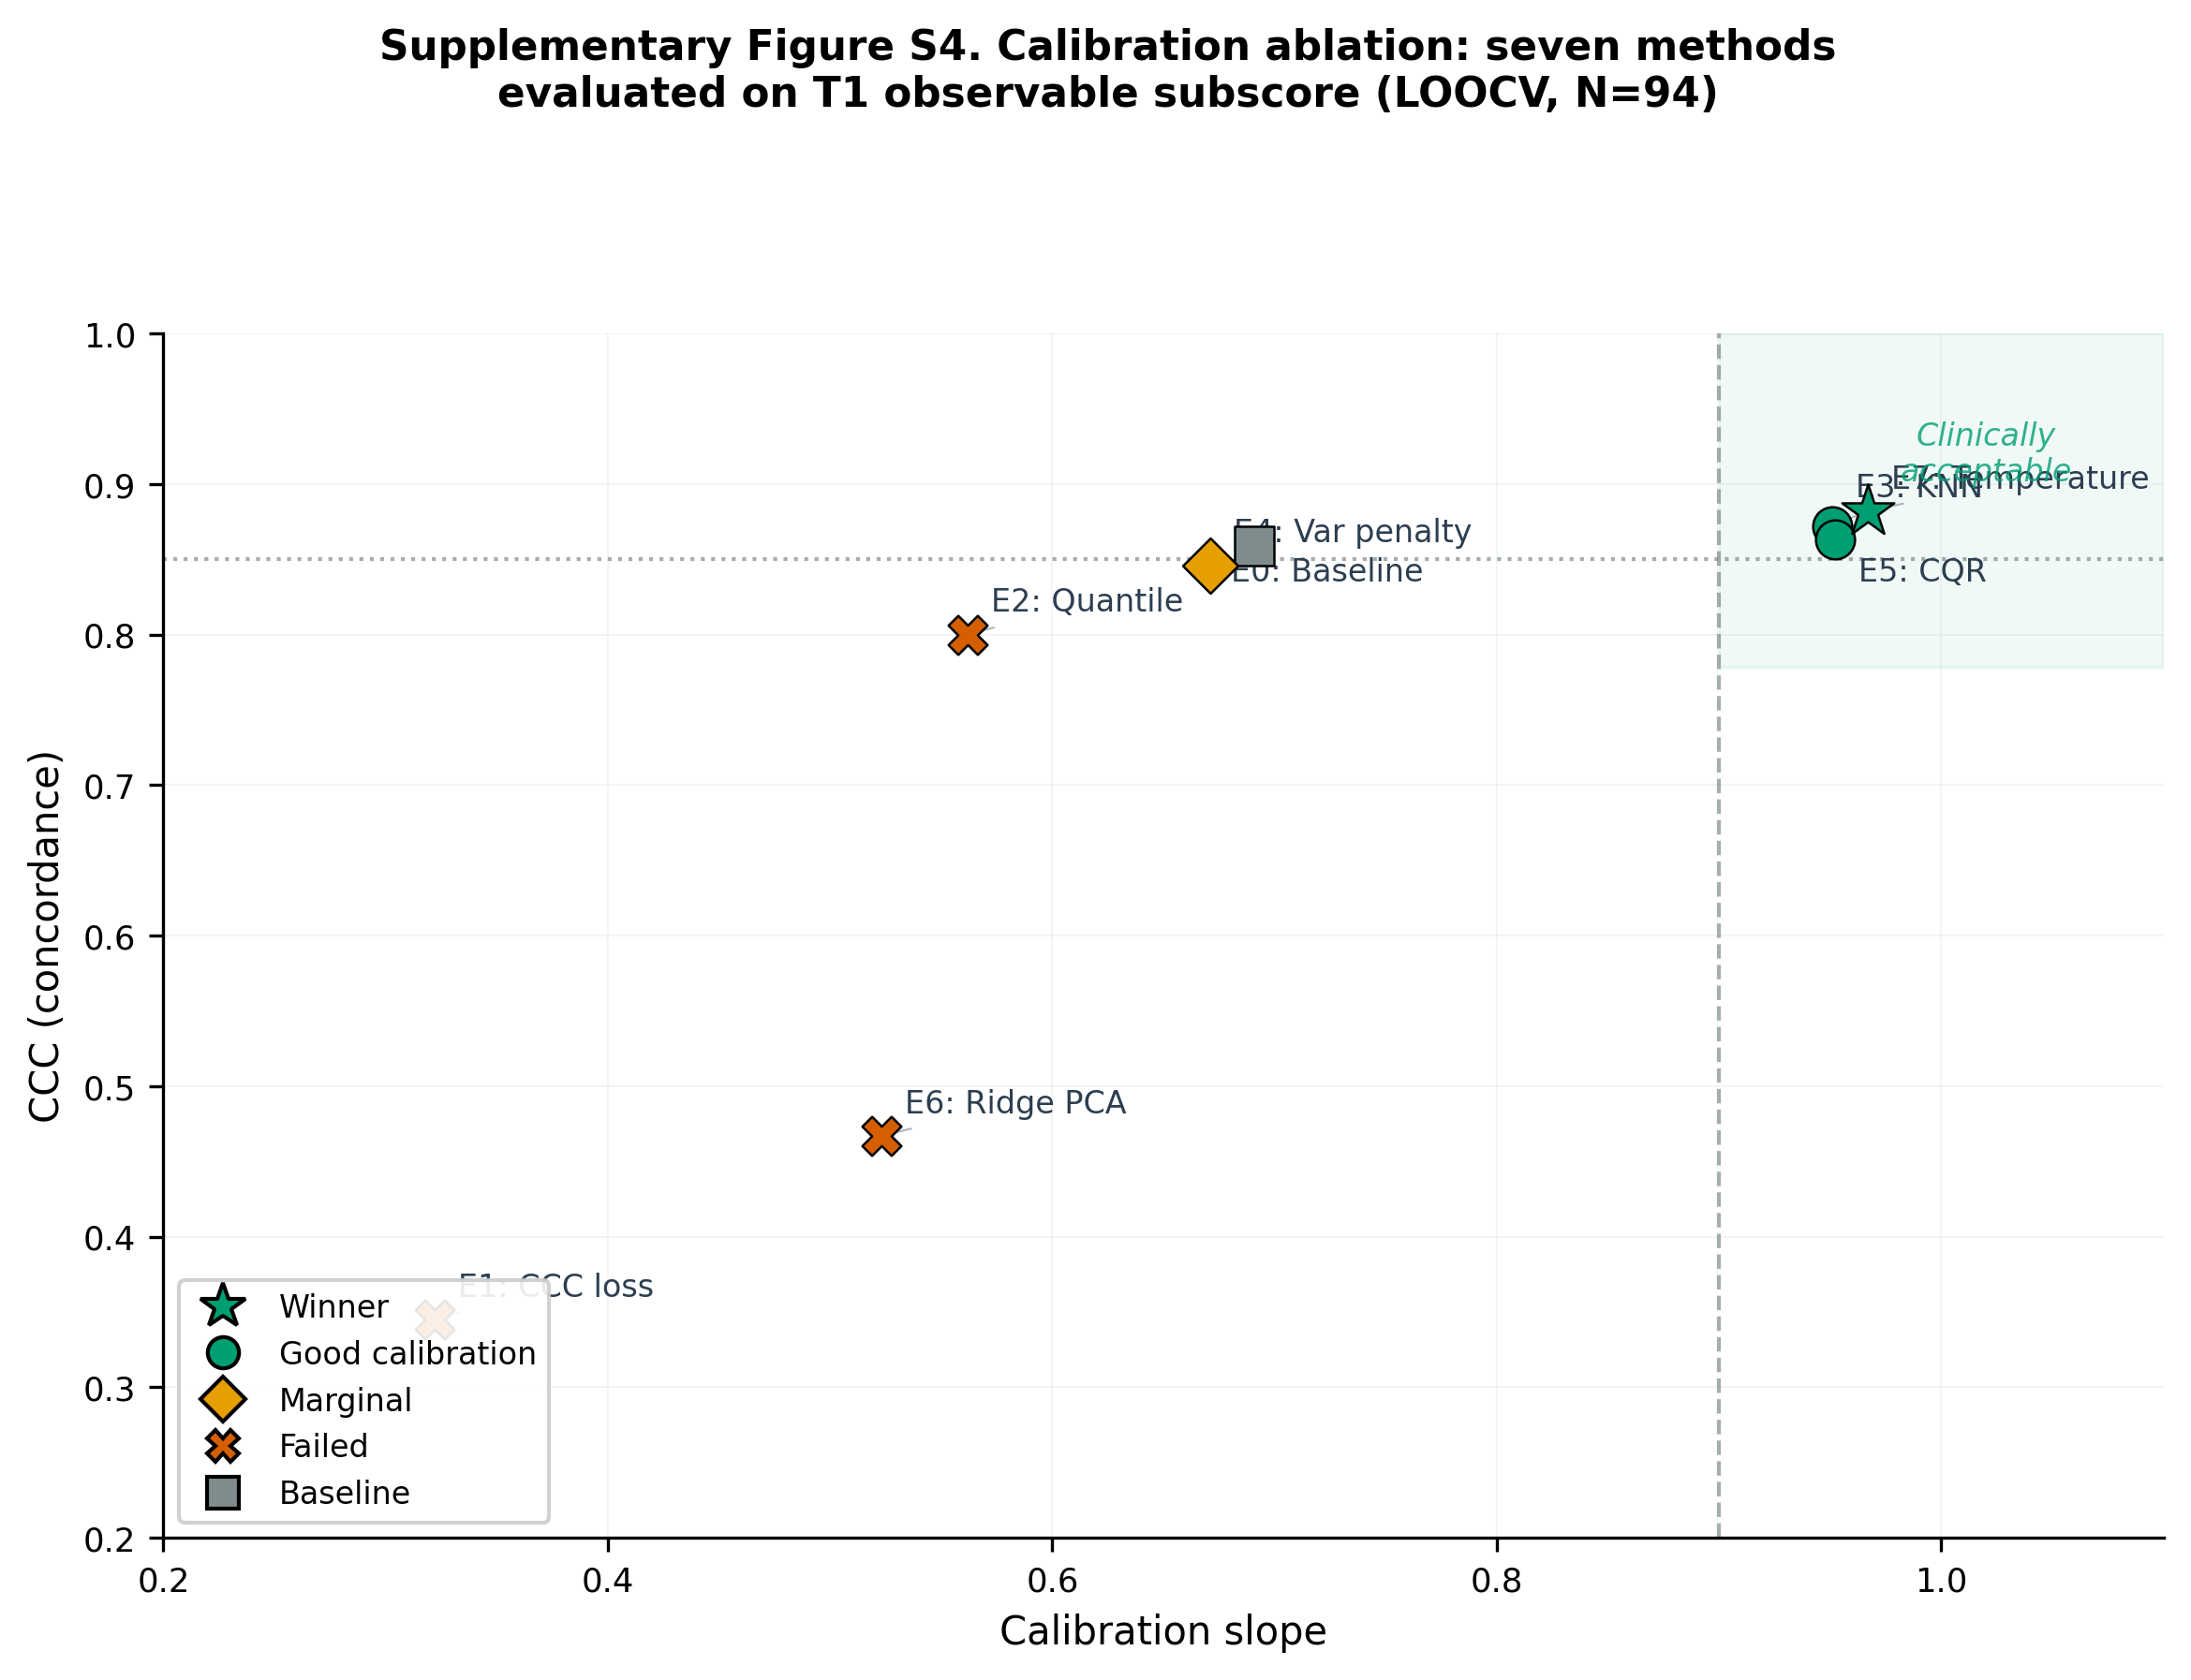
\includegraphics[width=0.9\linewidth]{19_supplementary_figure_s4.png}
\caption{\textbf{Figure~S4.} Calibration ablation: seven methods evaluated on T1 observable subscore (LOOCV, $N=94$). The upper-right quadrant (slope $>0.90$, CCC $>0.85$) represents the clinically acceptable zone. Only E3 (KNN), E5 (CQR), and E7 (temperature scaling) achieve both adequate calibration and concordance. E7 is selected for its simplicity (single parameter).}
\label{fig:s4calib}
\end{figure}

\begin{figure}[H]
\centering
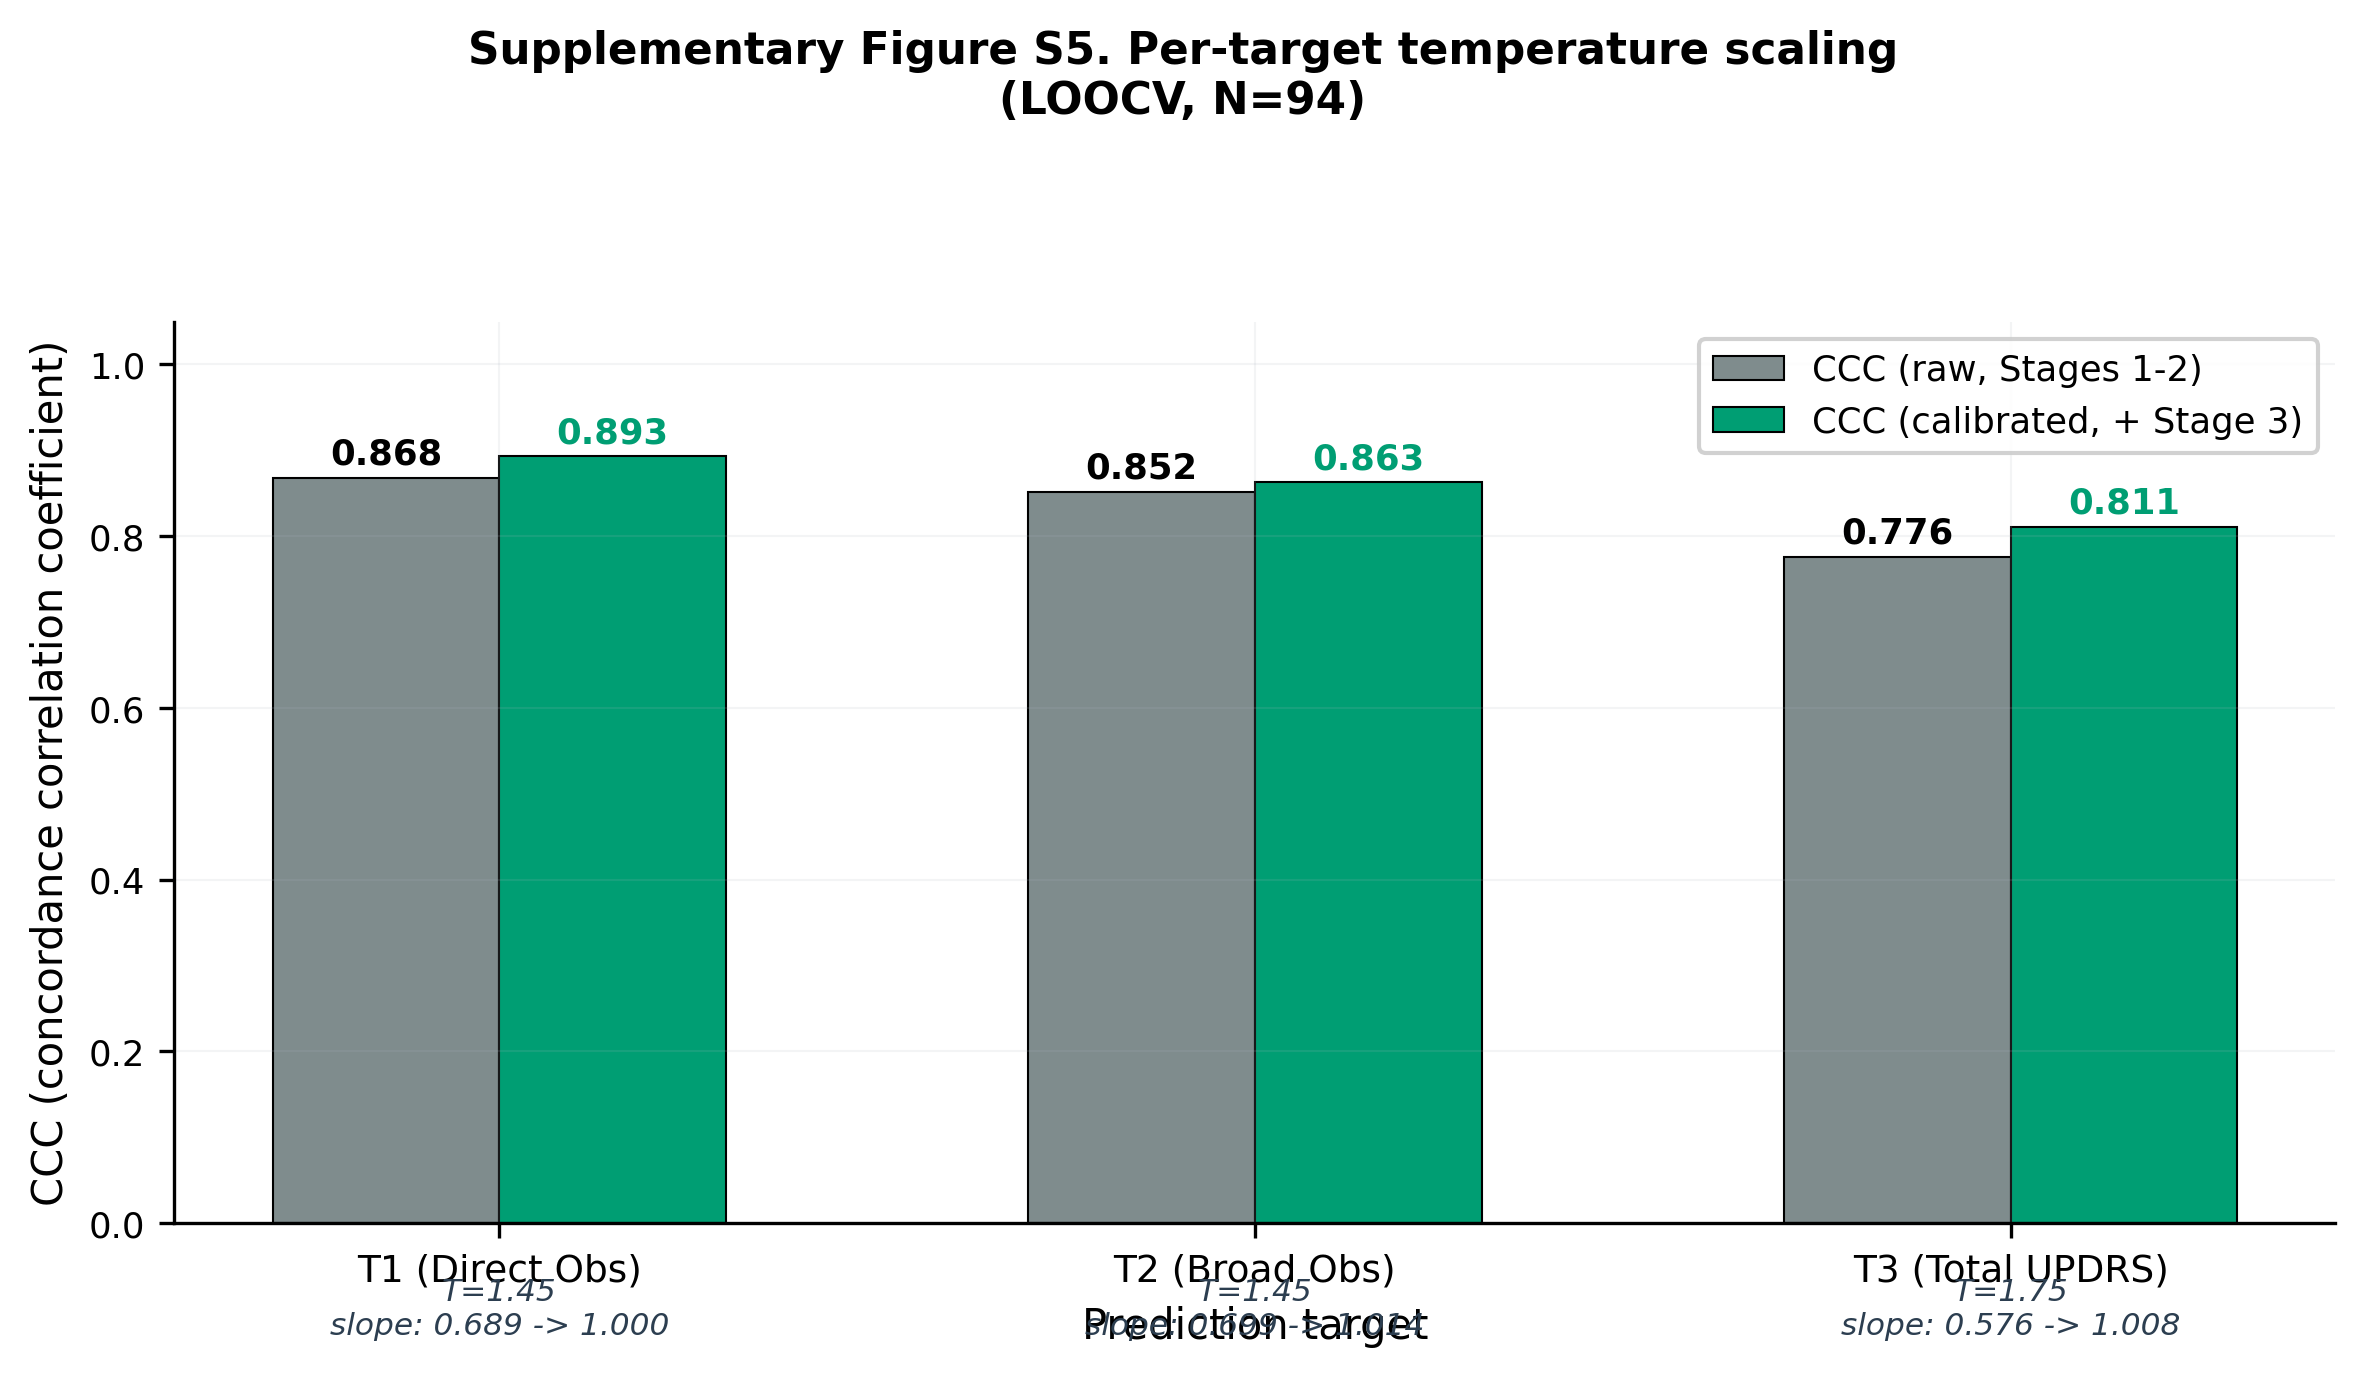
\includegraphics[width=0.9\linewidth]{20_supplementary_figure_s5.png}
\caption{\textbf{Figure~S5.} Per-target temperature scaling (LOOCV, $N=94$). Temperature $T$ is tuned independently per target to minimize $|\text{slope} - 1.0|$. All three targets show improved calibration slope ($>0.99$) with modest CCC gains. T1 and T2 require $T=1.45$; T3 requires $T=1.75$, reflecting greater raw compression for unobservable items.}
\label{fig:s5pertarget}
\end{figure}

\subsection*{S6: LOOCV Sensitivity Analysis}

To confirm that results are not sensitive to the choice of cross-validation protocol, we repeated the ordinal ranking evaluation using leave-one-out cross-validation (LOOCV, $N=94$). LOOCV results are consistent with the primary 5-fold analysis:

\begin{table}[H]
\centering
\caption{\textbf{Table~S7.} Protocol sensitivity: 5-fold CV vs LOOCV for ordinal ranking (PD-only).}
\label{tab:loocv}
\resizebox{\textwidth}{!}{%
\begin{tabular}{lrrrrrr}
\toprule
& \multicolumn{3}{c}{\textbf{5-fold CV ($N=95$)}} & \multicolumn{3}{c}{\textbf{LOOCV ($N=94$)}} \\
\cmidrule(lr){2-4}\cmidrule(lr){5-7}
\textbf{Target} & \textbf{CCC} & \textbf{MAE} & \textbf{$r$} & \textbf{CCC} & \textbf{MAE} & \textbf{$r$} \\
\midrule
T1 (direct obs) & \textbf{0.864} & 1.156 & 0.877 & 0.868 & 0.986 & 0.899 \\
T2 (broad obs)  & \textbf{0.831} & 1.162 & 0.847 & 0.852 & 1.334 & 0.873 \\
T3 (total)      & \textbf{0.807} & 4.464 & 0.877 & 0.776 & 4.646 & 0.827 \\
\bottomrule
\end{tabular}
}%
\tabnote{5-fold CV is the primary evaluation. T1 5-fold values include Stage~3 temperature scaling ($T=1.4$); T2 and T3 report Stages~1--2 only (temperature was tuned on T1). LOOCV is provided as sensitivity analysis (Stages~1--2 only for all targets). The close agreement between protocols confirms result robustness.}
\end{table}

\begin{table}[H]
\centering
\caption{\textbf{Table~S9.} Holm--Bonferroni corrected $p$-values across primary statistical tests.}
\label{tab:holm}
\begin{tabular}{lrrl}
\toprule
\textbf{Test} & \textbf{$p$ (raw)} & \textbf{$p$ (adjusted)} & \textbf{Sig.} \\
\midrule
P1\_fm\_vs\_v2\_median        & 0.4692   & 0.9384   & ns  \\
P1\_fm\_vs\_demo\_median      & 0.2991   & 0.8973   & ns  \\
P2\_permutation               & $<0.001$ & 0.0021   & **  \\
P2\_fm\_vs\_demo\_bootstrap   & 0.5924   & 0.9384   & ns  \\
P2\_partial\_corr             & $<0.001$ & 0.0021   & **  \\
P3\_ordering\_test            & 0.1721   & 0.6884   & ns  \\
P4\_spearman                  & $<0.001$ & $<0.001$ & *** \\
P4\_partial\_corr             & $<0.001$ & 0.0021   & **  \\
\bottomrule
\end{tabular}
\tabnote{Three tests survive correction: permutation (FM $>$ mean), Spearman severity ranking, and partial correlation (IMU signal beyond demographics).}
\end{table}

\begin{table}[H]
\centering
\caption{\textbf{Table~S10.} Three-level observability decomposition (baseline model, PD-only LOOCV).}
\label{tab:obsbaseline}
\small
\resizebox{\textwidth}{!}{%
\begin{tabular}{llrrrrrrrr}
\toprule
\textbf{Tier} & \textbf{Items} & \textbf{Max} & \textbf{$N$} & \textbf{MAE} & \textbf{nMAE\%} & \textbf{CCC} & \textbf{Slope} & \textbf{$r$} & \textbf{10-split MAE} \\
\midrule
Directly observable    & 3.9--3.14            & 24 & 94 & 1.77 & 7.4 & 0.560 & 0.401 & 0.667 & $1.72 \pm 0.33$ \\
Partially observable   & 3.5--3.8, 3.15--3.17 & 68 & 94 & 4.89 & 7.2 & 0.120 & 0.082 & 0.169 & $3.99 \pm 0.65$ \\
Not observable         & 3.1--3.4, 3.18       & 40 & 91 & 3.94 & 9.8 & 0.182 & 0.129 & 0.290 & $3.85 \pm 0.46$ \\
Binary observable      & 3.7--3.14            & 40 & 94 & 3.13 & 7.8 & 0.464 & 0.315 & 0.608 & --- \\
\bottomrule
\end{tabular}
}%
\tabnote{Baseline model (pre-ranking). LOOCV: PD-only, $N=91$--$94$. nMAE $=$ MAE / max score $\times 100$. Direct + partial + unobs $=$ total (reconstruction error $=0.0$).}
\end{table}

\end{document}
